\documentclass[twoside]{book}

% Packages required by doxygen
\usepackage{fixltx2e}
\usepackage{calc}
\usepackage{doxygen}
\usepackage[export]{adjustbox} % also loads graphicx
\usepackage{graphicx}
\usepackage[utf8]{inputenc}
\usepackage{makeidx}
\usepackage{multicol}
\usepackage{multirow}
\PassOptionsToPackage{warn}{textcomp}
\usepackage{textcomp}
\usepackage[nointegrals]{wasysym}
\usepackage[table]{xcolor}

% NLS support packages
\usepackage[french]{babel}

% Font selection
\usepackage[T1]{fontenc}
\usepackage[scaled=.90]{helvet}
\usepackage{courier}
\usepackage{amssymb}
\usepackage{sectsty}
\renewcommand{\familydefault}{\sfdefault}
\allsectionsfont{%
  \fontseries{bc}\selectfont%
  \color{darkgray}%
}
\renewcommand{\DoxyLabelFont}{%
  \fontseries{bc}\selectfont%
  \color{darkgray}%
}
\newcommand{\+}{\discretionary{\mbox{\scriptsize$\hookleftarrow$}}{}{}}

% Page & text layout
\usepackage{geometry}
\geometry{%
  a4paper,%
  top=2.5cm,%
  bottom=2.5cm,%
  left=2.5cm,%
  right=2.5cm%
}
\tolerance=750
\hfuzz=15pt
\hbadness=750
\setlength{\emergencystretch}{15pt}
\setlength{\parindent}{0cm}
\setlength{\parskip}{3ex plus 2ex minus 2ex}
\makeatletter
\renewcommand{\paragraph}{%
  \@startsection{paragraph}{4}{0ex}{-1.0ex}{1.0ex}{%
    \normalfont\normalsize\bfseries\SS@parafont%
  }%
}
\renewcommand{\subparagraph}{%
  \@startsection{subparagraph}{5}{0ex}{-1.0ex}{1.0ex}{%
    \normalfont\normalsize\bfseries\SS@subparafont%
  }%
}
\makeatother

% Headers & footers
\usepackage{fancyhdr}
\pagestyle{fancyplain}
\fancyhead[LE]{\fancyplain{}{\bfseries\thepage}}
\fancyhead[CE]{\fancyplain{}{}}
\fancyhead[RE]{\fancyplain{}{\bfseries\leftmark}}
\fancyhead[LO]{\fancyplain{}{\bfseries\rightmark}}
\fancyhead[CO]{\fancyplain{}{}}
\fancyhead[RO]{\fancyplain{}{\bfseries\thepage}}
\fancyfoot[LE]{\fancyplain{}{}}
\fancyfoot[CE]{\fancyplain{}{}}
\fancyfoot[RE]{\fancyplain{}{\bfseries\scriptsize Généré par Doxygen }}
\fancyfoot[LO]{\fancyplain{}{\bfseries\scriptsize Généré par Doxygen }}
\fancyfoot[CO]{\fancyplain{}{}}
\fancyfoot[RO]{\fancyplain{}{}}
\renewcommand{\footrulewidth}{0.4pt}
\renewcommand{\chaptermark}[1]{%
  \markboth{#1}{}%
}
\renewcommand{\sectionmark}[1]{%
  \markright{\thesection\ #1}%
}

% Indices & bibliography
\usepackage{natbib}
\usepackage[titles]{tocloft}
\setcounter{tocdepth}{3}
\setcounter{secnumdepth}{5}
\makeindex

% Hyperlinks (required, but should be loaded last)
\usepackage{ifpdf}
\ifpdf
  \usepackage[pdftex,pagebackref=true]{hyperref}
\else
  \usepackage[ps2pdf,pagebackref=true]{hyperref}
\fi
\hypersetup{%
  colorlinks=true,%
  linkcolor=blue,%
  citecolor=blue,%
  unicode%
}

% Custom commands
\newcommand{\clearemptydoublepage}{%
  \newpage{\pagestyle{empty}\cleardoublepage}%
}

\usepackage{caption}
\captionsetup{labelsep=space,justification=centering,font={bf},singlelinecheck=off,skip=4pt,position=top}

%===== C O N T E N T S =====

\begin{document}

% Titlepage & ToC
\hypersetup{pageanchor=false,
             bookmarksnumbered=true,
             pdfencoding=unicode
            }
\pagenumbering{roman}
\begin{titlepage}
\vspace*{7cm}
\begin{center}%
{\Large My Project \\[1ex]\large 0.\+01 }\\
\vspace*{1cm}
{\large Généré par Doxygen 1.8.11}\\
\end{center}
\end{titlepage}
\clearemptydoublepage
\tableofcontents
\clearemptydoublepage
\pagenumbering{arabic}
\hypersetup{pageanchor=true}

%--- Begin generated contents ---
\chapter{Liste des choses à faire}
\label{todo}
\hypertarget{todo}{}

\begin{DoxyRefList}
\item[\label{todo__todo000001}%
\hypertarget{todo__todo000001}{}%
Membre \hyperlink{main_8cpp_ae66f6b31b5ad750f1fe042a706a4e3d4}{main} ()]trouver un truc pour les accents 
\end{DoxyRefList}
\chapter{Index des modules}
\section{Modules}
Liste de tous les modules \+:\begin{DoxyCompactList}
\item \contentsline{section}{Module pour Application}{\pageref{group__application}}{}
\end{DoxyCompactList}

\chapter{Index des espaces de nommage}
\section{Liste des espaces de nommage}
Liste de tous les espaces de nommage avec une brève description\+:\begin{DoxyCompactList}
\item\contentsline{section}{\hyperlink{namespaceapp}{app} }{\pageref{namespaceapp}}{}
\item\contentsline{section}{\hyperlink{namespacegui}{gui} }{\pageref{namespacegui}}{}
\item\contentsline{section}{\hyperlink{namespacejeu}{jeu} }{\pageref{namespacejeu}}{}
\end{DoxyCompactList}

\chapter{Index hiérarchique}
\section{Hiérarchie des classes}
Cette liste d\textquotesingle{}héritage est classée approximativement par ordre alphabétique \+:\begin{DoxyCompactList}
\item \contentsline{section}{app\+:\+:Application}{\pageref{classapp_1_1_application}}{}
\item \contentsline{section}{app\+:\+:Config}{\pageref{classapp_1_1_config}}{}
\item Drawable\begin{DoxyCompactList}
\item \contentsline{section}{gui\+:\+:Gadget}{\pageref{classgui_1_1_gadget}}{}
\begin{DoxyCompactList}
\item \contentsline{section}{gui\+:\+:Bouton}{\pageref{classgui_1_1_bouton}}{}
\item \contentsline{section}{gui\+:\+:Fenetre}{\pageref{classgui_1_1_fenetre}}{}
\item \contentsline{section}{gui\+:\+:Gui}{\pageref{classgui_1_1_gui}}{}
\item \contentsline{section}{gui\+:\+:Image}{\pageref{classgui_1_1_image}}{}
\item \contentsline{section}{gui\+:\+:Interface\+Pheromones}{\pageref{classgui_1_1_interface_pheromones}}{}
\item \contentsline{section}{gui\+:\+:Label}{\pageref{classgui_1_1_label}}{}
\item \contentsline{section}{gui\+:\+:Vue}{\pageref{classgui_1_1_vue}}{}
\end{DoxyCompactList}
\item \contentsline{section}{jeu\+:\+:Etage}{\pageref{classjeu_1_1_etage}}{}
\item \contentsline{section}{jeu\+:\+:Jeu}{\pageref{classjeu_1_1_jeu}}{}
\item \contentsline{section}{jeu\+:\+:Plante\+Verte}{\pageref{classjeu_1_1_plante_verte}}{}
\item \contentsline{section}{jeu\+:\+:Terrain}{\pageref{classjeu_1_1_terrain}}{}
\end{DoxyCompactList}
\item \contentsline{section}{app\+:\+:Ecran}{\pageref{classapp_1_1_ecran}}{}
\begin{DoxyCompactList}
\item \contentsline{section}{app\+:\+:Ecran\+Accueil}{\pageref{classapp_1_1_ecran_accueil}}{}
\item \contentsline{section}{app\+:\+:Ecran\+Jeu}{\pageref{classapp_1_1_ecran_jeu}}{}
\end{DoxyCompactList}
\item \contentsline{section}{gui\+:\+:Fabrique}{\pageref{classgui_1_1_fabrique}}{}
\item \contentsline{section}{app\+:\+:Gestion\+\_\+ecrans}{\pageref{classapp_1_1_gestion__ecrans}}{}
\item Non\+Copyable\begin{DoxyCompactList}
\item \contentsline{section}{gui\+:\+:Gadget}{\pageref{classgui_1_1_gadget}}{}
\item \contentsline{section}{jeu\+:\+:Etage}{\pageref{classjeu_1_1_etage}}{}
\item \contentsline{section}{jeu\+:\+:Jeu}{\pageref{classjeu_1_1_jeu}}{}
\item \contentsline{section}{jeu\+:\+:Plante\+Verte}{\pageref{classjeu_1_1_plante_verte}}{}
\item \contentsline{section}{jeu\+:\+:Terrain}{\pageref{classjeu_1_1_terrain}}{}
\end{DoxyCompactList}
\item \contentsline{section}{app\+:\+:Resource\+Mgr$<$ R\+E\+S\+O\+U\+R\+CE, I\+D\+E\+N\+T\+I\+F\+I\+A\+NT $>$}{\pageref{classapp_1_1_resource_mgr}}{}
\item \contentsline{section}{app\+:\+:Resource\+Mgr$<$ sf\+:\+:Music, I\+D\+E\+N\+T\+I\+F\+I\+A\+NT $>$}{\pageref{classapp_1_1_resource_mgr_3_01sf_1_1_music_00_01_i_d_e_n_t_i_f_i_a_n_t_01_4}}{}
\item \contentsline{section}{gui\+:\+:Style}{\pageref{classgui_1_1_style}}{}
\item Transformable\begin{DoxyCompactList}
\item \contentsline{section}{gui\+:\+:Gadget}{\pageref{classgui_1_1_gadget}}{}
\item \contentsline{section}{jeu\+:\+:Plante\+Verte}{\pageref{classjeu_1_1_plante_verte}}{}
\end{DoxyCompactList}
\end{DoxyCompactList}

\chapter{Index des classes}
\section{Liste des classes}
Liste des classes, structures, unions et interfaces avec une brève description \+:\begin{DoxyCompactList}
\item\contentsline{section}{\hyperlink{classapp_1_1_application}{app\+::\+Application} \\*La classe de base du programme }{\pageref{classapp_1_1_application}}{}
\item\contentsline{section}{\hyperlink{classgui_1_1_bouton}{gui\+::\+Bouton} \\*Un bouton }{\pageref{classgui_1_1_bouton}}{}
\item\contentsline{section}{\hyperlink{classapp_1_1_config}{app\+::\+Config} \\*Contient les différents éléments de Configuration de l\textquotesingle{}application }{\pageref{classapp_1_1_config}}{}
\item\contentsline{section}{\hyperlink{classapp_1_1_ecran}{app\+::\+Ecran} \\*La classe virtuelle communues aux �crans }{\pageref{classapp_1_1_ecran}}{}
\item\contentsline{section}{\hyperlink{classapp_1_1_ecran_accueil}{app\+::\+Ecran\+Accueil} \\*\hyperlink{classapp_1_1_ecran}{Ecran} de démonstration }{\pageref{classapp_1_1_ecran_accueil}}{}
\item\contentsline{section}{\hyperlink{classapp_1_1_ecran_jeu}{app\+::\+Ecran\+Jeu} \\*\hyperlink{classapp_1_1_ecran}{Ecran} de jeu }{\pageref{classapp_1_1_ecran_jeu}}{}
\item\contentsline{section}{\hyperlink{classjeu_1_1_etage}{jeu\+::\+Etage} \\*Un seul �tage est visible � la fois. Compos� de sol, terre et vide. Chaque �tage g�re les collisions }{\pageref{classjeu_1_1_etage}}{}
\item\contentsline{section}{\hyperlink{classgui_1_1_fabrique}{gui\+::\+Fabrique} \\*La fabrique des gadget }{\pageref{classgui_1_1_fabrique}}{}
\item\contentsline{section}{\hyperlink{classgui_1_1_fenetre}{gui\+::\+Fenetre} \\*Une fen�tre encapsule des �l�ments d\textquotesingle{}interface }{\pageref{classgui_1_1_fenetre}}{}
\item\contentsline{section}{\hyperlink{classgui_1_1_gadget}{gui\+::\+Gadget} \\*Un gadget est la classe abstraite des �l�ments de l\textquotesingle{}interface }{\pageref{classgui_1_1_gadget}}{}
\item\contentsline{section}{\hyperlink{classapp_1_1_gestion__ecrans}{app\+::\+Gestion\+\_\+ecrans} \\*Gestionnaire des �crans }{\pageref{classapp_1_1_gestion__ecrans}}{}
\item\contentsline{section}{\hyperlink{classgui_1_1_gui}{gui\+::\+Gui} \\*Le \hyperlink{classgui_1_1_gui}{Gui} g�re l\textquotesingle{}ensemble des interactions homme-\/machine du jeu. D\textquotesingle{}un cot� un syst�me de fen�tre, boutons basique g�rant les diff�rents menus de l\textquotesingle{}appli. De l\textquotesingle{}autre, le menu ph�romones, syst�me central de l\textquotesingle{}interaction du joueur avec ses fourmis }{\pageref{classgui_1_1_gui}}{}
\item\contentsline{section}{\hyperlink{classgui_1_1_image}{gui\+::\+Image} \\*Une simple image }{\pageref{classgui_1_1_image}}{}
\item\contentsline{section}{\hyperlink{classgui_1_1_interface_pheromones}{gui\+::\+Interface\+Pheromones} \\*L\textquotesingle{}interface des ph�romones }{\pageref{classgui_1_1_interface_pheromones}}{}
\item\contentsline{section}{\hyperlink{classjeu_1_1_jeu}{jeu\+::\+Jeu} \\*La classe g�n�ral du jeu, g�re le jeu de mani�re global. popo autre ligne l� aussi }{\pageref{classjeu_1_1_jeu}}{}
\item\contentsline{section}{\hyperlink{classgui_1_1_label}{gui\+::\+Label} \\*Un simple label }{\pageref{classgui_1_1_label}}{}
\item\contentsline{section}{\hyperlink{classjeu_1_1_plante_verte}{jeu\+::\+Plante\+Verte} \\*Une plante verte apporte de la nourriture aux fourmis et autres insectes du biome }{\pageref{classjeu_1_1_plante_verte}}{}
\item\contentsline{section}{\hyperlink{classapp_1_1_resource_mgr}{app\+::\+Resource\+Mgr$<$ R\+E\+S\+O\+U\+R\+C\+E, I\+D\+E\+N\+T\+I\+F\+I\+A\+N\+T $>$} \\*Manager de ressource (polices, images) }{\pageref{classapp_1_1_resource_mgr}}{}
\item\contentsline{section}{\hyperlink{classapp_1_1_resource_mgr_3_01sf_1_1_music_00_01_i_d_e_n_t_i_f_i_a_n_t_01_4}{app\+::\+Resource\+Mgr$<$ sf\+::\+Music, I\+D\+E\+N\+T\+I\+F\+I\+A\+N\+T $>$} \\*Manager de ressource (music) }{\pageref{classapp_1_1_resource_mgr_3_01sf_1_1_music_00_01_i_d_e_n_t_i_f_i_a_n_t_01_4}}{}
\item\contentsline{section}{\hyperlink{classgui_1_1_style}{gui\+::\+Style} \\*Regroupe les couleurs, polices et style de texte de l\textquotesingle{}interface }{\pageref{classgui_1_1_style}}{}
\item\contentsline{section}{\hyperlink{classjeu_1_1_terrain}{jeu\+::\+Terrain} \\*Le terrain est le champs d\textquotesingle{}�volution des fourmis et autres �l�ments du biome. Compos� de plusieurs �tages ( 2? ou 3? ), il est repr�sent� en 2D avec une profondeur repr�sentant les �tages. Le "tilemap\textquotesingle{} est au niveau du pixel }{\pageref{classjeu_1_1_terrain}}{}
\item\contentsline{section}{\hyperlink{classgui_1_1_vue}{gui\+::\+Vue} \\*Une vue S\+F\+ML }{\pageref{classgui_1_1_vue}}{}
\end{DoxyCompactList}

\chapter{Index des fichiers}
\section{Liste des fichiers}
Liste de tous les fichiers avec une brève description \+:\begin{DoxyCompactList}
\item\contentsline{section}{C\+:/\+Users/kris/\+One\+Drive/recherche Biome/01 -\/ code/code/\hyperlink{main_8cpp}{main.\+cpp} }{\pageref{main_8cpp}}{}
\item\contentsline{section}{C\+:/\+Users/kris/\+One\+Drive/recherche Biome/01 -\/ code/code/include/appli/\hyperlink{_application_8h}{Application.\+h} \\*La classe principale du programme }{\pageref{_application_8h}}{}
\item\contentsline{section}{C\+:/\+Users/kris/\+One\+Drive/recherche Biome/01 -\/ code/code/include/appli/\hyperlink{_config_8h}{Config.\+h} }{\pageref{_config_8h}}{}
\item\contentsline{section}{C\+:/\+Users/kris/\+One\+Drive/recherche Biome/01 -\/ code/code/include/appli/\hyperlink{_ecran_8h}{Ecran.\+h} }{\pageref{_ecran_8h}}{}
\item\contentsline{section}{C\+:/\+Users/kris/\+One\+Drive/recherche Biome/01 -\/ code/code/include/appli/\hyperlink{_gestion__ecrans_8h}{Gestion\+\_\+ecrans.\+h} }{\pageref{_gestion__ecrans_8h}}{}
\item\contentsline{section}{C\+:/\+Users/kris/\+One\+Drive/recherche Biome/01 -\/ code/code/include/appli/\hyperlink{_resource_mgr_8h}{Resource\+Mgr.\+h} }{\pageref{_resource_mgr_8h}}{}
\item\contentsline{section}{C\+:/\+Users/kris/\+One\+Drive/recherche Biome/01 -\/ code/code/include/appli/\hyperlink{_resource_mgr_8inl}{Resource\+Mgr.\+inl} }{\pageref{_resource_mgr_8inl}}{}
\item\contentsline{section}{C\+:/\+Users/kris/\+One\+Drive/recherche Biome/01 -\/ code/code/include/appli/ecrans/\hyperlink{_ecran_accueil_8h}{Ecran\+Accueil.\+h} }{\pageref{_ecran_accueil_8h}}{}
\item\contentsline{section}{C\+:/\+Users/kris/\+One\+Drive/recherche Biome/01 -\/ code/code/include/appli/ecrans/\hyperlink{_ecran_jeu_8h}{Ecran\+Jeu.\+h} }{\pageref{_ecran_jeu_8h}}{}
\item\contentsline{section}{C\+:/\+Users/kris/\+One\+Drive/recherche Biome/01 -\/ code/code/include/gui/\hyperlink{_bouton_8h}{Bouton.\+h} }{\pageref{_bouton_8h}}{}
\item\contentsline{section}{C\+:/\+Users/kris/\+One\+Drive/recherche Biome/01 -\/ code/code/include/gui/\hyperlink{_fabrique_8h}{Fabrique.\+h} }{\pageref{_fabrique_8h}}{}
\item\contentsline{section}{C\+:/\+Users/kris/\+One\+Drive/recherche Biome/01 -\/ code/code/include/gui/\hyperlink{_fenetre_8h}{Fenetre.\+h} }{\pageref{_fenetre_8h}}{}
\item\contentsline{section}{C\+:/\+Users/kris/\+One\+Drive/recherche Biome/01 -\/ code/code/include/gui/\hyperlink{_gadget_8h}{Gadget.\+h} }{\pageref{_gadget_8h}}{}
\item\contentsline{section}{C\+:/\+Users/kris/\+One\+Drive/recherche Biome/01 -\/ code/code/include/gui/\hyperlink{_gui_8h}{Gui.\+h} }{\pageref{_gui_8h}}{}
\item\contentsline{section}{C\+:/\+Users/kris/\+One\+Drive/recherche Biome/01 -\/ code/code/include/gui/\hyperlink{_image_8h}{Image.\+h} }{\pageref{_image_8h}}{}
\item\contentsline{section}{C\+:/\+Users/kris/\+One\+Drive/recherche Biome/01 -\/ code/code/include/gui/\hyperlink{_interface_pheromones_8h}{Interface\+Pheromones.\+h} }{\pageref{_interface_pheromones_8h}}{}
\item\contentsline{section}{C\+:/\+Users/kris/\+One\+Drive/recherche Biome/01 -\/ code/code/include/gui/\hyperlink{_label_8h}{Label.\+h} }{\pageref{_label_8h}}{}
\item\contentsline{section}{C\+:/\+Users/kris/\+One\+Drive/recherche Biome/01 -\/ code/code/include/gui/\hyperlink{_style_8h}{Style.\+h} }{\pageref{_style_8h}}{}
\item\contentsline{section}{C\+:/\+Users/kris/\+One\+Drive/recherche Biome/01 -\/ code/code/include/gui/\hyperlink{_vue_8h}{Vue.\+h} }{\pageref{_vue_8h}}{}
\item\contentsline{section}{C\+:/\+Users/kris/\+One\+Drive/recherche Biome/01 -\/ code/code/include/jeu/\hyperlink{_etage_8h}{Etage.\+h} }{\pageref{_etage_8h}}{}
\item\contentsline{section}{C\+:/\+Users/kris/\+One\+Drive/recherche Biome/01 -\/ code/code/include/jeu/\hyperlink{_jeu_8h}{Jeu.\+h} }{\pageref{_jeu_8h}}{}
\item\contentsline{section}{C\+:/\+Users/kris/\+One\+Drive/recherche Biome/01 -\/ code/code/include/jeu/\hyperlink{_plante_verte_8h}{Plante\+Verte.\+h} }{\pageref{_plante_verte_8h}}{}
\item\contentsline{section}{C\+:/\+Users/kris/\+One\+Drive/recherche Biome/01 -\/ code/code/include/jeu/\hyperlink{_terrain_8h}{Terrain.\+h} }{\pageref{_terrain_8h}}{}
\item\contentsline{section}{C\+:/\+Users/kris/\+One\+Drive/recherche Biome/01 -\/ code/code/include/outils/\hyperlink{_utilitaires_8h}{Utilitaires.\+h} }{\pageref{_utilitaires_8h}}{}
\item\contentsline{section}{C\+:/\+Users/kris/\+One\+Drive/recherche Biome/01 -\/ code/code/include/outils/\hyperlink{_utilitaires_8inl}{Utilitaires.\+inl} }{\pageref{_utilitaires_8inl}}{}
\end{DoxyCompactList}

\chapter{Documentation des modules}
\hypertarget{group__application}{}\section{Module pour Application}
\label{group__application}\index{Module pour Application@{Module pour Application}}
\subsection*{Classes}
\begin{DoxyCompactItemize}
\item 
class \hyperlink{classapp_1_1_application}{app\+::\+Application}
\begin{DoxyCompactList}\small\item\em La classe de base du programme. \end{DoxyCompactList}\item 
class \hyperlink{classapp_1_1_config}{app\+::\+Config}
\begin{DoxyCompactList}\small\item\em Contient les différents éléments de Configuration de l\textquotesingle{}application. \end{DoxyCompactList}\item 
class \hyperlink{classapp_1_1_ecran}{app\+::\+Ecran}
\begin{DoxyCompactList}\small\item\em La classe virtuelle communues aux �crans. \end{DoxyCompactList}\item 
class \hyperlink{classapp_1_1_gestion__ecrans}{app\+::\+Gestion\+\_\+ecrans}
\begin{DoxyCompactList}\small\item\em Gestionnaire des �crans. \end{DoxyCompactList}\item 
class \hyperlink{classapp_1_1_resource_mgr}{app\+::\+Resource\+Mgr$<$ R\+E\+S\+O\+U\+R\+C\+E, I\+D\+E\+N\+T\+I\+F\+I\+A\+N\+T $>$}
\begin{DoxyCompactList}\small\item\em Manager de ressource (polices, images). \end{DoxyCompactList}\end{DoxyCompactItemize}


\subsection{Description détaillée}
G�re les diff�rents �crans du programme (�cran d\textquotesingle{}introduction, accueil, pause, �cran du jeu ....)

Peut-\/�tre pour tester d\textquotesingle{}autre trucs, comme la bibilo d\textquotesingle{}interface graphique... ou comme base pour demarrer un nouveau projet.

Manipule les diff�rents �crans de l\textquotesingle{}application � l\textquotesingle{}aide d\textquotesingle{}une boucle infernalede type \+: \begin{DoxyItemize}
\item Ecouter les �venements utilisateurs ( claviers, cliques...). \item Actualiser les parametres de tout les �l�ments ( position, couleurs, points de vies ... ). \item Dessiner les �l�ments dans la fenetre\end{DoxyItemize}
C\textquotesingle{}est le gestionnaire des �crans ( m\+\_\+ecrans app\+:Gestion\+\_\+\+Ecrans ) qui se charge du traitement de la pile des �crans.

Quand il n\textquotesingle{}y a plus d\textquotesingle{}�crans dans la pile, l\textquotesingle{}application se ferme.

\begin{DoxySeeAlso}{Voir également}
\hyperlink{classapp_1_1_ecran}{app\+::\+Ecran}, app\+::\+Ecran\+Demo, \hyperlink{classapp_1_1_gestion__ecrans}{app\+::\+Gestion\+\_\+ecrans} 
\end{DoxySeeAlso}

\chapter{Documentation des espaces de nommage}
\hypertarget{namespaceapp}{}\section{Référence de l\textquotesingle{}espace de nommage app}
\label{namespaceapp}\index{app@{app}}
\subsection*{Classes}
\begin{DoxyCompactItemize}
\item 
class \hyperlink{classapp_1_1_application}{Application}
\begin{DoxyCompactList}\small\item\em La classe de base du programme. \end{DoxyCompactList}\item 
class \hyperlink{classapp_1_1_config}{Config}
\begin{DoxyCompactList}\small\item\em Contient les différents éléments de Configuration de l\textquotesingle{}application. \end{DoxyCompactList}\item 
class \hyperlink{classapp_1_1_ecran}{Ecran}
\begin{DoxyCompactList}\small\item\em La classe virtuelle communues aux �crans. \end{DoxyCompactList}\item 
class \hyperlink{classapp_1_1_ecran_accueil}{Ecran\+Accueil}
\begin{DoxyCompactList}\small\item\em \hyperlink{classapp_1_1_ecran}{Ecran} de démonstration. \end{DoxyCompactList}\item 
class \hyperlink{classapp_1_1_ecran_jeu}{Ecran\+Jeu}
\begin{DoxyCompactList}\small\item\em \hyperlink{classapp_1_1_ecran}{Ecran} de jeu. \end{DoxyCompactList}\item 
class \hyperlink{classapp_1_1_gestion__ecrans}{Gestion\+\_\+ecrans}
\begin{DoxyCompactList}\small\item\em Gestionnaire des �crans. \end{DoxyCompactList}\item 
class \hyperlink{classapp_1_1_resource_mgr}{Resource\+Mgr}
\begin{DoxyCompactList}\small\item\em Manager de ressource (polices, images). \end{DoxyCompactList}\item 
class \hyperlink{classapp_1_1_resource_mgr_3_01sf_1_1_music_00_01_i_d_e_n_t_i_f_i_a_n_t_01_4}{Resource\+Mgr$<$ sf\+::\+Music, I\+D\+E\+N\+T\+I\+F\+I\+A\+N\+T $>$}
\begin{DoxyCompactList}\small\item\em Manager de ressource (music). \end{DoxyCompactList}\end{DoxyCompactItemize}

\hypertarget{namespacegui}{}\section{Référence de l\textquotesingle{}espace de nommage gui}
\label{namespacegui}\index{gui@{gui}}
\subsection*{Classes}
\begin{DoxyCompactItemize}
\item 
class \hyperlink{classgui_1_1_bouton}{Bouton}
\begin{DoxyCompactList}\small\item\em Un bouton. \end{DoxyCompactList}\item 
class \hyperlink{classgui_1_1_fabrique}{Fabrique}
\begin{DoxyCompactList}\small\item\em La fabrique des gadget. \end{DoxyCompactList}\item 
class \hyperlink{classgui_1_1_fenetre}{Fenetre}
\begin{DoxyCompactList}\small\item\em Une fen�tre encapsule des �l�ments d\textquotesingle{}interface. \end{DoxyCompactList}\item 
class \hyperlink{classgui_1_1_gadget}{Gadget}
\begin{DoxyCompactList}\small\item\em Un gadget est la classe abstraite des �l�ments de l\textquotesingle{}interface. \end{DoxyCompactList}\item 
class \hyperlink{classgui_1_1_gui}{Gui}
\begin{DoxyCompactList}\small\item\em Le \hyperlink{classgui_1_1_gui}{Gui} g�re l\textquotesingle{}ensemble des interactions homme-\/machine du jeu. D\textquotesingle{}un cot� un syst�me de fen�tre, boutons basique g�rant les diff�rents menus de l\textquotesingle{}appli. De l\textquotesingle{}autre, le menu ph�romones, syst�me central de l\textquotesingle{}interaction du joueur avec ses fourmis. \end{DoxyCompactList}\item 
class \hyperlink{classgui_1_1_image}{Image}
\begin{DoxyCompactList}\small\item\em Une simple image. \end{DoxyCompactList}\item 
class \hyperlink{classgui_1_1_interface_pheromones}{Interface\+Pheromones}
\begin{DoxyCompactList}\small\item\em L\textquotesingle{}interface des ph�romones. \end{DoxyCompactList}\item 
class \hyperlink{classgui_1_1_label}{Label}
\begin{DoxyCompactList}\small\item\em Un simple label. \end{DoxyCompactList}\item 
class \hyperlink{classgui_1_1_style}{Style}
\begin{DoxyCompactList}\small\item\em Regroupe les couleurs, polices et style de texte de l\textquotesingle{}interface. \end{DoxyCompactList}\item 
class \hyperlink{classgui_1_1_vue}{Vue}
\begin{DoxyCompactList}\small\item\em Une vue S\+F\+ML. \end{DoxyCompactList}\end{DoxyCompactItemize}

\hypertarget{namespacejeu}{}\section{Référence de l\textquotesingle{}espace de nommage jeu}
\label{namespacejeu}\index{jeu@{jeu}}
\subsection*{Classes}
\begin{DoxyCompactItemize}
\item 
class \hyperlink{classjeu_1_1_etage}{Etage}
\begin{DoxyCompactList}\small\item\em Un seul �tage est visible � la fois. Compos� de sol, terre et vide. Chaque �tage g�re les collisions. \end{DoxyCompactList}\item 
class \hyperlink{classjeu_1_1_jeu}{Jeu}
\begin{DoxyCompactList}\small\item\em La classe g�n�ral du jeu, g�re le jeu de mani�re global. popo autre ligne l� aussi. \end{DoxyCompactList}\item 
class \hyperlink{classjeu_1_1_plante_verte}{Plante\+Verte}
\begin{DoxyCompactList}\small\item\em Une plante verte apporte de la nourriture aux fourmis et autres insectes du biome. \end{DoxyCompactList}\item 
class \hyperlink{classjeu_1_1_terrain}{Terrain}
\begin{DoxyCompactList}\small\item\em Le terrain est le champs d\textquotesingle{}�volution des fourmis et autres �l�ments du biome. Compos� de plusieurs �tages ( 2? ou 3? ), il est repr�sent� en 2D avec une profondeur repr�sentant les �tages. Le "tilemap\textquotesingle{} est au niveau du pixel. \end{DoxyCompactList}\end{DoxyCompactItemize}

\chapter{Documentation des classes}
\hypertarget{classapp_1_1_application}{}\section{Référence de la classe app\+:\+:Application}
\label{classapp_1_1_application}\index{app\+::\+Application@{app\+::\+Application}}


La classe de base du programme.  




{\ttfamily \#include $<$Application.\+h$>$}

\subsection*{Types publics}
\begin{DoxyCompactItemize}
\item 
enum \hyperlink{classapp_1_1_application_af23b16d902265e5140a3c29f9f2a45a7}{Ecrans} \{ \hyperlink{classapp_1_1_application_af23b16d902265e5140a3c29f9f2a45a7a73bf7ecf1c9b44c4f3022d48f187cd70}{Accueil}, 
\hyperlink{classapp_1_1_application_af23b16d902265e5140a3c29f9f2a45a7a4f69f619f9ff3c77e312f52cefeba3e6}{Jeu}
 \}
\end{DoxyCompactItemize}
\subsection*{Fonctions membres publiques}
\begin{DoxyCompactItemize}
\item 
\hyperlink{classapp_1_1_application_a3c480be05f51b91e648b2f6533a32f1b}{Application} ()
\begin{DoxyCompactList}\small\item\em Constructeur. \end{DoxyCompactList}\item 
virtual \hyperlink{classapp_1_1_application_a6d1fee4f8c8fb3d33470f605c179def9}{$\sim$\+Application} ()
\begin{DoxyCompactList}\small\item\em Destructeur. \end{DoxyCompactList}\item 
void \hyperlink{classapp_1_1_application_ace29cf983643a2cc74cb52b19483620d}{changer\+Ecran} (\hyperlink{classapp_1_1_application_af23b16d902265e5140a3c29f9f2a45a7}{Ecrans} ecran)
\begin{DoxyCompactList}\small\item\em Changer d\textquotesingle{}�cran. \end{DoxyCompactList}\item 
void \hyperlink{classapp_1_1_application_a266215c22bb94757ac0b338a3abc3daa}{ajouter\+Ecran} (\hyperlink{classapp_1_1_application_af23b16d902265e5140a3c29f9f2a45a7}{Ecrans} ecran)
\begin{DoxyCompactList}\small\item\em ajouter un �cran \end{DoxyCompactList}\item 
void \hyperlink{classapp_1_1_application_a6cbc17d5a777730d7811e874182fd11a}{retirer\+Ecran} ()
\begin{DoxyCompactList}\small\item\em retirer un �cran \end{DoxyCompactList}\item 
void \hyperlink{classapp_1_1_application_ae375e0fdeb21265f93cff8958a26f95d}{executer} ()
\begin{DoxyCompactList}\small\item\em La boucle principale. \end{DoxyCompactList}\item 
void \hyperlink{classapp_1_1_application_aee4bdeeb44c6b2a943acc8e651b0ff83}{traiter\+\_\+evenements} ()
\begin{DoxyCompactList}\small\item\em La gestion des �v�nements utilisateurs. \end{DoxyCompactList}\item 
void \hyperlink{classapp_1_1_application_ad10d5a33f82b7fc224e3d0c7c8bf57b2}{actualiser} (sf\+::\+Time deltaT)
\begin{DoxyCompactList}\small\item\em Actualiser les �l�ments. \end{DoxyCompactList}\item 
void \hyperlink{classapp_1_1_application_a03b3bac56e523faa9669622eadd237f8}{dessiner} ()
\begin{DoxyCompactList}\small\item\em Rendre les �l�ments. \end{DoxyCompactList}\item 
sf\+::\+Render\+Window $\ast$ \hyperlink{classapp_1_1_application_a8636afdcd2019c1358560d92e156e68c}{get\+Fenetre} ()
\begin{DoxyCompactList}\small\item\em renvois la fenetre sfml de l\textquotesingle{}application \end{DoxyCompactList}\end{DoxyCompactItemize}


\subsection{Description détaillée}
La classe de base du programme. 

\subsection{Documentation des énumérations membres}
\index{app\+::\+Application@{app\+::\+Application}!Ecrans@{Ecrans}}
\index{Ecrans@{Ecrans}!app\+::\+Application@{app\+::\+Application}}
\subsubsection[{\texorpdfstring{Ecrans}{Ecrans}}]{\setlength{\rightskip}{0pt plus 5cm}enum {\bf app\+::\+Application\+::\+Ecrans}}\hypertarget{classapp_1_1_application_af23b16d902265e5140a3c29f9f2a45a7}{}\label{classapp_1_1_application_af23b16d902265e5140a3c29f9f2a45a7}
\begin{Desc}
\item[Valeurs énumérées]\par
\begin{description}
\index{Accueil@{Accueil}!app\+::\+Application@{app\+::\+Application}}\index{app\+::\+Application@{app\+::\+Application}!Accueil@{Accueil}}\item[{\em 
Accueil\hypertarget{classapp_1_1_application_af23b16d902265e5140a3c29f9f2a45a7a73bf7ecf1c9b44c4f3022d48f187cd70}{}\label{classapp_1_1_application_af23b16d902265e5140a3c29f9f2a45a7a73bf7ecf1c9b44c4f3022d48f187cd70}
}]\index{Jeu@{Jeu}!app\+::\+Application@{app\+::\+Application}}\index{app\+::\+Application@{app\+::\+Application}!Jeu@{Jeu}}\item[{\em 
Jeu\hypertarget{classapp_1_1_application_af23b16d902265e5140a3c29f9f2a45a7a4f69f619f9ff3c77e312f52cefeba3e6}{}\label{classapp_1_1_application_af23b16d902265e5140a3c29f9f2a45a7a4f69f619f9ff3c77e312f52cefeba3e6}
}]\end{description}
\end{Desc}


\subsection{Documentation des constructeurs et destructeur}
\index{app\+::\+Application@{app\+::\+Application}!Application@{Application}}
\index{Application@{Application}!app\+::\+Application@{app\+::\+Application}}
\subsubsection[{\texorpdfstring{Application()}{Application()}}]{\setlength{\rightskip}{0pt plus 5cm}app\+::\+Application\+::\+Application (
\begin{DoxyParamCaption}
{}
\end{DoxyParamCaption}
)}\hypertarget{classapp_1_1_application_a3c480be05f51b91e648b2f6533a32f1b}{}\label{classapp_1_1_application_a3c480be05f51b91e648b2f6533a32f1b}


Constructeur. 

\index{app\+::\+Application@{app\+::\+Application}!````~Application@{$\sim$\+Application}}
\index{````~Application@{$\sim$\+Application}!app\+::\+Application@{app\+::\+Application}}
\subsubsection[{\texorpdfstring{$\sim$\+Application()}{~Application()}}]{\setlength{\rightskip}{0pt plus 5cm}virtual app\+::\+Application\+::$\sim$\+Application (
\begin{DoxyParamCaption}
{}
\end{DoxyParamCaption}
)\hspace{0.3cm}{\ttfamily [virtual]}}\hypertarget{classapp_1_1_application_a6d1fee4f8c8fb3d33470f605c179def9}{}\label{classapp_1_1_application_a6d1fee4f8c8fb3d33470f605c179def9}


Destructeur. 



\subsection{Documentation des fonctions membres}
\index{app\+::\+Application@{app\+::\+Application}!actualiser@{actualiser}}
\index{actualiser@{actualiser}!app\+::\+Application@{app\+::\+Application}}
\subsubsection[{\texorpdfstring{actualiser(sf\+::\+Time delta\+T)}{actualiser(sf::Time deltaT)}}]{\setlength{\rightskip}{0pt plus 5cm}void app\+::\+Application\+::actualiser (
\begin{DoxyParamCaption}
\item[{sf\+::\+Time}]{deltaT}
\end{DoxyParamCaption}
)}\hypertarget{classapp_1_1_application_ad10d5a33f82b7fc224e3d0c7c8bf57b2}{}\label{classapp_1_1_application_ad10d5a33f82b7fc224e3d0c7c8bf57b2}


Actualiser les �l�ments. 

Actualiser les diff�rents �l�ments du ou des �crans actifs. 
\begin{DoxyParams}{Paramètres}
{\em deltaT} & Un {\itshape float} qui indique le delta du temps �coul� depuis la derni�re actualisation. pour ponderer les mouvements en fonction du temps et ainsi avoir une ind�pendance entre animation et frame rate. \\
\hline
\end{DoxyParams}
\index{app\+::\+Application@{app\+::\+Application}!ajouter\+Ecran@{ajouter\+Ecran}}
\index{ajouter\+Ecran@{ajouter\+Ecran}!app\+::\+Application@{app\+::\+Application}}
\subsubsection[{\texorpdfstring{ajouter\+Ecran(\+Ecrans ecran)}{ajouterEcran(Ecrans ecran)}}]{\setlength{\rightskip}{0pt plus 5cm}void app\+::\+Application\+::ajouter\+Ecran (
\begin{DoxyParamCaption}
\item[{{\bf Ecrans}}]{ecran}
\end{DoxyParamCaption}
)}\hypertarget{classapp_1_1_application_a266215c22bb94757ac0b338a3abc3daa}{}\label{classapp_1_1_application_a266215c22bb94757ac0b338a3abc3daa}


ajouter un �cran 

\begin{DoxyReturn}{Renvoie}
Rien 
\end{DoxyReturn}
\index{app\+::\+Application@{app\+::\+Application}!changer\+Ecran@{changer\+Ecran}}
\index{changer\+Ecran@{changer\+Ecran}!app\+::\+Application@{app\+::\+Application}}
\subsubsection[{\texorpdfstring{changer\+Ecran(\+Ecrans ecran)}{changerEcran(Ecrans ecran)}}]{\setlength{\rightskip}{0pt plus 5cm}void app\+::\+Application\+::changer\+Ecran (
\begin{DoxyParamCaption}
\item[{{\bf Ecrans}}]{ecran}
\end{DoxyParamCaption}
)}\hypertarget{classapp_1_1_application_ace29cf983643a2cc74cb52b19483620d}{}\label{classapp_1_1_application_ace29cf983643a2cc74cb52b19483620d}


Changer d\textquotesingle{}�cran. 

\begin{DoxyReturn}{Renvoie}
Rien 
\end{DoxyReturn}
\index{app\+::\+Application@{app\+::\+Application}!dessiner@{dessiner}}
\index{dessiner@{dessiner}!app\+::\+Application@{app\+::\+Application}}
\subsubsection[{\texorpdfstring{dessiner()}{dessiner()}}]{\setlength{\rightskip}{0pt plus 5cm}void app\+::\+Application\+::dessiner (
\begin{DoxyParamCaption}
{}
\end{DoxyParamCaption}
)}\hypertarget{classapp_1_1_application_a03b3bac56e523faa9669622eadd237f8}{}\label{classapp_1_1_application_a03b3bac56e523faa9669622eadd237f8}


Rendre les �l�ments. 

Dessiner les diff�rents �l�ments du ou des �crans actifs. \begin{DoxyReturn}{Renvoie}
Rien 
\end{DoxyReturn}
\index{app\+::\+Application@{app\+::\+Application}!executer@{executer}}
\index{executer@{executer}!app\+::\+Application@{app\+::\+Application}}
\subsubsection[{\texorpdfstring{executer()}{executer()}}]{\setlength{\rightskip}{0pt plus 5cm}void app\+::\+Application\+::executer (
\begin{DoxyParamCaption}
{}
\end{DoxyParamCaption}
)}\hypertarget{classapp_1_1_application_ae375e0fdeb21265f93cff8958a26f95d}{}\label{classapp_1_1_application_ae375e0fdeb21265f93cff8958a26f95d}


La boucle principale. 

\begin{DoxyReturn}{Renvoie}
Rien 
\end{DoxyReturn}
\index{app\+::\+Application@{app\+::\+Application}!get\+Fenetre@{get\+Fenetre}}
\index{get\+Fenetre@{get\+Fenetre}!app\+::\+Application@{app\+::\+Application}}
\subsubsection[{\texorpdfstring{get\+Fenetre()}{getFenetre()}}]{\setlength{\rightskip}{0pt plus 5cm}sf\+::\+Render\+Window$\ast$ app\+::\+Application\+::get\+Fenetre (
\begin{DoxyParamCaption}
{}
\end{DoxyParamCaption}
)}\hypertarget{classapp_1_1_application_a8636afdcd2019c1358560d92e156e68c}{}\label{classapp_1_1_application_a8636afdcd2019c1358560d92e156e68c}


renvois la fenetre sfml de l\textquotesingle{}application 

\begin{DoxyReturn}{Renvoie}
la fenetre sfml de l\textquotesingle{}application 
\end{DoxyReturn}
\index{app\+::\+Application@{app\+::\+Application}!retirer\+Ecran@{retirer\+Ecran}}
\index{retirer\+Ecran@{retirer\+Ecran}!app\+::\+Application@{app\+::\+Application}}
\subsubsection[{\texorpdfstring{retirer\+Ecran()}{retirerEcran()}}]{\setlength{\rightskip}{0pt plus 5cm}void app\+::\+Application\+::retirer\+Ecran (
\begin{DoxyParamCaption}
{}
\end{DoxyParamCaption}
)}\hypertarget{classapp_1_1_application_a6cbc17d5a777730d7811e874182fd11a}{}\label{classapp_1_1_application_a6cbc17d5a777730d7811e874182fd11a}


retirer un �cran 

\begin{DoxyReturn}{Renvoie}
Rien 
\end{DoxyReturn}
\index{app\+::\+Application@{app\+::\+Application}!traiter\+\_\+evenements@{traiter\+\_\+evenements}}
\index{traiter\+\_\+evenements@{traiter\+\_\+evenements}!app\+::\+Application@{app\+::\+Application}}
\subsubsection[{\texorpdfstring{traiter\+\_\+evenements()}{traiter_evenements()}}]{\setlength{\rightskip}{0pt plus 5cm}void app\+::\+Application\+::traiter\+\_\+evenements (
\begin{DoxyParamCaption}
{}
\end{DoxyParamCaption}
)}\hypertarget{classapp_1_1_application_aee4bdeeb44c6b2a943acc8e651b0ff83}{}\label{classapp_1_1_application_aee4bdeeb44c6b2a943acc8e651b0ff83}


La gestion des �v�nements utilisateurs. 

G�re les entr�es claviers, souris, fenetre ... \begin{DoxyReturn}{Renvoie}
Rien 
\end{DoxyReturn}


La documentation de cette classe a été générée à partir du fichier suivant \+:\begin{DoxyCompactItemize}
\item 
C\+:/\+Users/kris/\+One\+Drive/recherche Biome/01 -\/ code/code/include/appli/\hyperlink{_application_8h}{Application.\+h}\end{DoxyCompactItemize}

\hypertarget{classgui_1_1_bouton}{}\section{Référence de la classe gui\+:\+:Bouton}
\label{classgui_1_1_bouton}\index{gui\+::\+Bouton@{gui\+::\+Bouton}}


Un bouton.  




{\ttfamily \#include $<$Bouton.\+h$>$}



Graphe d\textquotesingle{}héritage de gui\+:\+:Bouton\+:\nopagebreak
\begin{figure}[H]
\begin{center}
\leavevmode
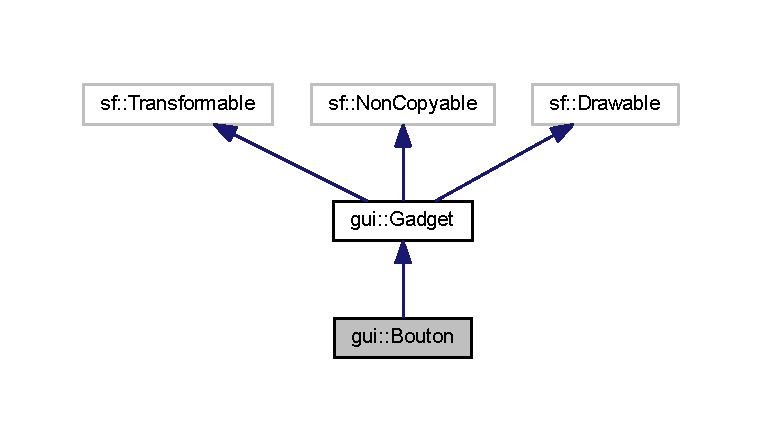
\includegraphics[width=350pt]{classgui_1_1_bouton__inherit__graph}
\end{center}
\end{figure}


Graphe de collaboration de gui\+:\+:Bouton\+:\nopagebreak
\begin{figure}[H]
\begin{center}
\leavevmode
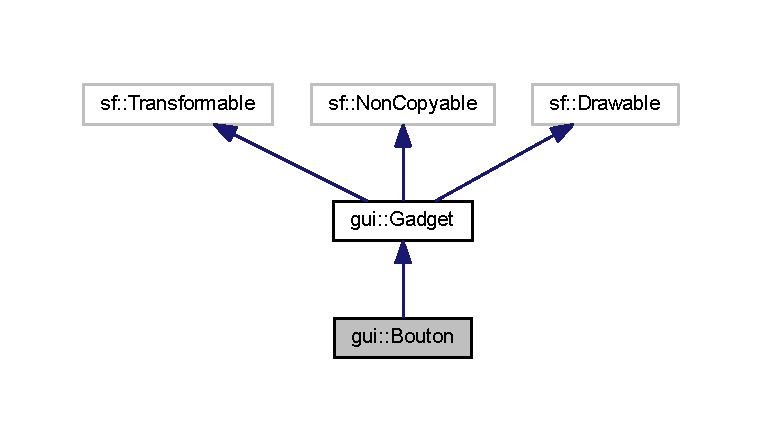
\includegraphics[width=350pt]{classgui_1_1_bouton__coll__graph}
\end{center}
\end{figure}
\subsection*{Fonctions membres publiques}
\begin{DoxyCompactItemize}
\item 
void \hyperlink{classgui_1_1_bouton_aafa7200ca277e63020cce724d164fa0d}{traiter\+Evenements} (sf\+::\+Event evenement)
\begin{DoxyCompactList}\small\item\em Traitement des �venements clavier ou souris. \end{DoxyCompactList}\item 
void \hyperlink{classgui_1_1_bouton_a2255d73ed2ea825e61279148c004884e}{actualiser} ()
\begin{DoxyCompactList}\small\item\em Actualiser les �l�ments de l\textquotesingle{}interface. \end{DoxyCompactList}\item 
virtual void \hyperlink{classgui_1_1_bouton_ae1ae117fb6e67dc7446eeb16c172ea14}{draw} (sf\+::\+Render\+Target \&target, sf\+::\+Render\+States states) const 
\begin{DoxyCompactList}\small\item\em Dessine tout les �l�ments de l\textquotesingle{}interface. \end{DoxyCompactList}\end{DoxyCompactItemize}


\subsection{Description détaillée}
Un bouton. 

\subsection{Documentation des fonctions membres}
\index{gui\+::\+Bouton@{gui\+::\+Bouton}!actualiser@{actualiser}}
\index{actualiser@{actualiser}!gui\+::\+Bouton@{gui\+::\+Bouton}}
\subsubsection[{\texorpdfstring{actualiser()}{actualiser()}}]{\setlength{\rightskip}{0pt plus 5cm}void gui\+::\+Bouton\+::actualiser (
\begin{DoxyParamCaption}
{}
\end{DoxyParamCaption}
)}\hypertarget{classgui_1_1_bouton_a2255d73ed2ea825e61279148c004884e}{}\label{classgui_1_1_bouton_a2255d73ed2ea825e61279148c004884e}


Actualiser les �l�ments de l\textquotesingle{}interface. 

\index{gui\+::\+Bouton@{gui\+::\+Bouton}!draw@{draw}}
\index{draw@{draw}!gui\+::\+Bouton@{gui\+::\+Bouton}}
\subsubsection[{\texorpdfstring{draw(sf\+::\+Render\+Target \&target, sf\+::\+Render\+States states) const }{draw(sf::RenderTarget &target, sf::RenderStates states) const }}]{\setlength{\rightskip}{0pt plus 5cm}virtual void gui\+::\+Bouton\+::draw (
\begin{DoxyParamCaption}
\item[{sf\+::\+Render\+Target \&}]{target, }
\item[{sf\+::\+Render\+States}]{states}
\end{DoxyParamCaption}
) const\hspace{0.3cm}{\ttfamily [virtual]}}\hypertarget{classgui_1_1_bouton_ae1ae117fb6e67dc7446eeb16c172ea14}{}\label{classgui_1_1_bouton_ae1ae117fb6e67dc7446eeb16c172ea14}


Dessine tout les �l�ments de l\textquotesingle{}interface. 


\begin{DoxyParams}{Paramètres}
{\em target} & \\
\hline
{\em states} & \\
\hline
\end{DoxyParams}


Réimplémentée à partir de \hyperlink{classgui_1_1_gadget_a57b0c75601c7f6e0d43370013ae8c111}{gui\+::\+Gadget}.

\index{gui\+::\+Bouton@{gui\+::\+Bouton}!traiter\+Evenements@{traiter\+Evenements}}
\index{traiter\+Evenements@{traiter\+Evenements}!gui\+::\+Bouton@{gui\+::\+Bouton}}
\subsubsection[{\texorpdfstring{traiter\+Evenements(sf\+::\+Event evenement)}{traiterEvenements(sf::Event evenement)}}]{\setlength{\rightskip}{0pt plus 5cm}void gui\+::\+Bouton\+::traiter\+Evenements (
\begin{DoxyParamCaption}
\item[{sf\+::\+Event}]{evenement}
\end{DoxyParamCaption}
)}\hypertarget{classgui_1_1_bouton_aafa7200ca277e63020cce724d164fa0d}{}\label{classgui_1_1_bouton_aafa7200ca277e63020cce724d164fa0d}


Traitement des �venements clavier ou souris. 


\begin{DoxyParams}{Paramètres}
{\em evenement} & L\textquotesingle{}�venemnt � tratier. \\
\hline
\end{DoxyParams}


La documentation de cette classe a été générée à partir du fichier suivant \+:\begin{DoxyCompactItemize}
\item 
C\+:/\+Users/kris/\+One\+Drive/recherche Biome/01 -\/ code/code/include/gui/\hyperlink{_bouton_8h}{Bouton.\+h}\end{DoxyCompactItemize}

\hypertarget{classapp_1_1_config}{}\section{Référence de la classe app\+:\+:Config}
\label{classapp_1_1_config}\index{app\+::\+Config@{app\+::\+Config}}


Contient les différents éléments de Configuration de l\textquotesingle{}application.  




{\ttfamily \#include $<$Config.\+h$>$}

\subsection*{Types publics}
\begin{DoxyCompactItemize}
\item 
enum \hyperlink{classapp_1_1_config_ac576a323feff0b9aaa6aecd40e038049}{Polices} \+: int \{ \hyperlink{classapp_1_1_config_ac576a323feff0b9aaa6aecd40e038049a759ba1bca9923fc3b3e61b9e0edd154a}{police\+\_\+1}, 
\hyperlink{classapp_1_1_config_ac576a323feff0b9aaa6aecd40e038049abd01fcbe87968783a525da9dc5ef0f21}{police\+\_\+2}, 
\hyperlink{classapp_1_1_config_ac576a323feff0b9aaa6aecd40e038049aa9e5b356892159d1526d850436f9186e}{log}
 \}\begin{DoxyCompactList}\small\item\em listes les polices enregistrable dans le manager de polices \end{DoxyCompactList}
\item 
enum \hyperlink{classapp_1_1_config_ab0fd2b7fe87a4b68c93d2a4a7209beda}{Styles} \+: int \{ \hyperlink{classapp_1_1_config_ab0fd2b7fe87a4b68c93d2a4a7209bedaa02fd230360f0a9b4e42a24c2e826e2a7}{root}, 
\hyperlink{classapp_1_1_config_ab0fd2b7fe87a4b68c93d2a4a7209bedaa853b0170848ebe1bb8aa66895283a816}{Bouton}, 
\hyperlink{classapp_1_1_config_ab0fd2b7fe87a4b68c93d2a4a7209bedaa1297561847b1b84d487c3a875f5f8f6a}{Fenetre}
 \}\begin{DoxyCompactList}\small\item\em listes les styles (\hyperlink{classgui_1_1_style}{gui\+::\+Style}) enregistrable dans la pile des Styles \end{DoxyCompactList}
\item 
enum \hyperlink{classapp_1_1_config_a457412fb51e1853408f2201a69471e32}{Skins} \+: int \{ \hyperlink{classapp_1_1_config_a457412fb51e1853408f2201a69471e32abb0a28eb4da75e2aadaf74b6d9aa2d4e}{Skin1}
 \}\begin{DoxyCompactList}\small\item\em listes les skins (gui\+::\+Skin) enregistrable dans la pile des skins. \end{DoxyCompactList}
\end{DoxyCompactItemize}
\subsection*{Fonctions membres publiques}
\begin{DoxyCompactItemize}
\item 
\hyperlink{classapp_1_1_config_a6b5877b87cbfef7bb28ed405dfa3ea62}{Config} ()
\begin{DoxyCompactList}\small\item\em Constructeur. \end{DoxyCompactList}\item 
virtual \hyperlink{classapp_1_1_config_af8bea439b3dd6daa60079937d43b0dcb}{$\sim$\+Config} ()
\begin{DoxyCompactList}\small\item\em Destructeur. \end{DoxyCompactList}\end{DoxyCompactItemize}
\subsection*{Fonctions membres publiques statiques}
\begin{DoxyCompactItemize}
\item 
static void \hyperlink{classapp_1_1_config_a8680abec2844bbb045614662a218b5d5}{init} ()
\begin{DoxyCompactList}\small\item\em Initialiser les differents élément. \end{DoxyCompactList}\item 
static sf\+::\+Time \hyperlink{classapp_1_1_config_a379b1f1ac039e8c2cb92567b994fe74c}{get\+Duree\+Image} ()
\begin{DoxyCompactList}\small\item\em recuperer la durée d\textquotesingle{}une image, Duree\+Image = 1.\+f / 60.\+f à 60\+Fps. \end{DoxyCompactList}\end{DoxyCompactItemize}


\subsection{Description détaillée}
Contient les différents éléments de Configuration de l\textquotesingle{}application. 

Configuration des textures, sons, musiques polices, tailles, couleurs ....

\begin{DoxySeeAlso}{Voir également}
\hyperlink{classapp_1_1_ecran}{app\+::\+Ecran}, \hyperlink{classapp_1_1_gestion__ecrans}{app\+::\+Gestion\+\_\+ecrans} 
\end{DoxySeeAlso}


\subsection{Documentation des énumérations membres}
\index{app\+::\+Config@{app\+::\+Config}!Polices@{Polices}}
\index{Polices@{Polices}!app\+::\+Config@{app\+::\+Config}}
\subsubsection[{\texorpdfstring{Polices}{Polices}}]{\setlength{\rightskip}{0pt plus 5cm}enum {\bf app\+::\+Config\+::\+Polices} \+: int}\hypertarget{classapp_1_1_config_ac576a323feff0b9aaa6aecd40e038049}{}\label{classapp_1_1_config_ac576a323feff0b9aaa6aecd40e038049}


listes les polices enregistrable dans le manager de polices 

\begin{Desc}
\item[Valeurs énumérées]\par
\begin{description}
\index{police\+\_\+1@{police\+\_\+1}!app\+::\+Config@{app\+::\+Config}}\index{app\+::\+Config@{app\+::\+Config}!police\+\_\+1@{police\+\_\+1}}\item[{\em 
police\+\_\+1\hypertarget{classapp_1_1_config_ac576a323feff0b9aaa6aecd40e038049a759ba1bca9923fc3b3e61b9e0edd154a}{}\label{classapp_1_1_config_ac576a323feff0b9aaa6aecd40e038049a759ba1bca9923fc3b3e61b9e0edd154a}
}]\index{police\+\_\+2@{police\+\_\+2}!app\+::\+Config@{app\+::\+Config}}\index{app\+::\+Config@{app\+::\+Config}!police\+\_\+2@{police\+\_\+2}}\item[{\em 
police\+\_\+2\hypertarget{classapp_1_1_config_ac576a323feff0b9aaa6aecd40e038049abd01fcbe87968783a525da9dc5ef0f21}{}\label{classapp_1_1_config_ac576a323feff0b9aaa6aecd40e038049abd01fcbe87968783a525da9dc5ef0f21}
}]\index{log@{log}!app\+::\+Config@{app\+::\+Config}}\index{app\+::\+Config@{app\+::\+Config}!log@{log}}\item[{\em 
log\hypertarget{classapp_1_1_config_ac576a323feff0b9aaa6aecd40e038049aa9e5b356892159d1526d850436f9186e}{}\label{classapp_1_1_config_ac576a323feff0b9aaa6aecd40e038049aa9e5b356892159d1526d850436f9186e}
}]\end{description}
\end{Desc}
\index{app\+::\+Config@{app\+::\+Config}!Skins@{Skins}}
\index{Skins@{Skins}!app\+::\+Config@{app\+::\+Config}}
\subsubsection[{\texorpdfstring{Skins}{Skins}}]{\setlength{\rightskip}{0pt plus 5cm}enum {\bf app\+::\+Config\+::\+Skins} \+: int}\hypertarget{classapp_1_1_config_a457412fb51e1853408f2201a69471e32}{}\label{classapp_1_1_config_a457412fb51e1853408f2201a69471e32}


listes les skins (gui\+::\+Skin) enregistrable dans la pile des skins. 

\begin{Desc}
\item[Valeurs énumérées]\par
\begin{description}
\index{Skin1@{Skin1}!app\+::\+Config@{app\+::\+Config}}\index{app\+::\+Config@{app\+::\+Config}!Skin1@{Skin1}}\item[{\em 
Skin1\hypertarget{classapp_1_1_config_a457412fb51e1853408f2201a69471e32abb0a28eb4da75e2aadaf74b6d9aa2d4e}{}\label{classapp_1_1_config_a457412fb51e1853408f2201a69471e32abb0a28eb4da75e2aadaf74b6d9aa2d4e}
}]\end{description}
\end{Desc}
\index{app\+::\+Config@{app\+::\+Config}!Styles@{Styles}}
\index{Styles@{Styles}!app\+::\+Config@{app\+::\+Config}}
\subsubsection[{\texorpdfstring{Styles}{Styles}}]{\setlength{\rightskip}{0pt plus 5cm}enum {\bf app\+::\+Config\+::\+Styles} \+: int}\hypertarget{classapp_1_1_config_ab0fd2b7fe87a4b68c93d2a4a7209beda}{}\label{classapp_1_1_config_ab0fd2b7fe87a4b68c93d2a4a7209beda}


listes les styles (\hyperlink{classgui_1_1_style}{gui\+::\+Style}) enregistrable dans la pile des Styles 

\begin{Desc}
\item[Valeurs énumérées]\par
\begin{description}
\index{root@{root}!app\+::\+Config@{app\+::\+Config}}\index{app\+::\+Config@{app\+::\+Config}!root@{root}}\item[{\em 
root\hypertarget{classapp_1_1_config_ab0fd2b7fe87a4b68c93d2a4a7209bedaa02fd230360f0a9b4e42a24c2e826e2a7}{}\label{classapp_1_1_config_ab0fd2b7fe87a4b68c93d2a4a7209bedaa02fd230360f0a9b4e42a24c2e826e2a7}
}]\index{Bouton@{Bouton}!app\+::\+Config@{app\+::\+Config}}\index{app\+::\+Config@{app\+::\+Config}!Bouton@{Bouton}}\item[{\em 
Bouton\hypertarget{classapp_1_1_config_ab0fd2b7fe87a4b68c93d2a4a7209bedaa853b0170848ebe1bb8aa66895283a816}{}\label{classapp_1_1_config_ab0fd2b7fe87a4b68c93d2a4a7209bedaa853b0170848ebe1bb8aa66895283a816}
}]\index{Fenetre@{Fenetre}!app\+::\+Config@{app\+::\+Config}}\index{app\+::\+Config@{app\+::\+Config}!Fenetre@{Fenetre}}\item[{\em 
Fenetre\hypertarget{classapp_1_1_config_ab0fd2b7fe87a4b68c93d2a4a7209bedaa1297561847b1b84d487c3a875f5f8f6a}{}\label{classapp_1_1_config_ab0fd2b7fe87a4b68c93d2a4a7209bedaa1297561847b1b84d487c3a875f5f8f6a}
}]\end{description}
\end{Desc}


\subsection{Documentation des constructeurs et destructeur}
\index{app\+::\+Config@{app\+::\+Config}!Config@{Config}}
\index{Config@{Config}!app\+::\+Config@{app\+::\+Config}}
\subsubsection[{\texorpdfstring{Config()}{Config()}}]{\setlength{\rightskip}{0pt plus 5cm}app\+::\+Config\+::\+Config (
\begin{DoxyParamCaption}
{}
\end{DoxyParamCaption}
)}\hypertarget{classapp_1_1_config_a6b5877b87cbfef7bb28ed405dfa3ea62}{}\label{classapp_1_1_config_a6b5877b87cbfef7bb28ed405dfa3ea62}


Constructeur. 

\index{app\+::\+Config@{app\+::\+Config}!````~Config@{$\sim$\+Config}}
\index{````~Config@{$\sim$\+Config}!app\+::\+Config@{app\+::\+Config}}
\subsubsection[{\texorpdfstring{$\sim$\+Config()}{~Config()}}]{\setlength{\rightskip}{0pt plus 5cm}virtual app\+::\+Config\+::$\sim$\+Config (
\begin{DoxyParamCaption}
{}
\end{DoxyParamCaption}
)\hspace{0.3cm}{\ttfamily [virtual]}}\hypertarget{classapp_1_1_config_af8bea439b3dd6daa60079937d43b0dcb}{}\label{classapp_1_1_config_af8bea439b3dd6daa60079937d43b0dcb}


Destructeur. 



\subsection{Documentation des fonctions membres}
\index{app\+::\+Config@{app\+::\+Config}!get\+Duree\+Image@{get\+Duree\+Image}}
\index{get\+Duree\+Image@{get\+Duree\+Image}!app\+::\+Config@{app\+::\+Config}}
\subsubsection[{\texorpdfstring{get\+Duree\+Image()}{getDureeImage()}}]{\setlength{\rightskip}{0pt plus 5cm}static sf\+::\+Time app\+::\+Config\+::get\+Duree\+Image (
\begin{DoxyParamCaption}
{}
\end{DoxyParamCaption}
)\hspace{0.3cm}{\ttfamily [static]}}\hypertarget{classapp_1_1_config_a379b1f1ac039e8c2cb92567b994fe74c}{}\label{classapp_1_1_config_a379b1f1ac039e8c2cb92567b994fe74c}


recuperer la durée d\textquotesingle{}une image, Duree\+Image = 1.\+f / 60.\+f à 60\+Fps. 

\index{app\+::\+Config@{app\+::\+Config}!init@{init}}
\index{init@{init}!app\+::\+Config@{app\+::\+Config}}
\subsubsection[{\texorpdfstring{init()}{init()}}]{\setlength{\rightskip}{0pt plus 5cm}static void app\+::\+Config\+::init (
\begin{DoxyParamCaption}
{}
\end{DoxyParamCaption}
)\hspace{0.3cm}{\ttfamily [static]}}\hypertarget{classapp_1_1_config_a8680abec2844bbb045614662a218b5d5}{}\label{classapp_1_1_config_a8680abec2844bbb045614662a218b5d5}


Initialiser les differents élément. 

\begin{DoxyItemize}
\item les textures \item les polices \item les styles \item les sons (à prévoir) \item les musiques (à prévoir) \end{DoxyItemize}


La documentation de cette classe a été générée à partir du fichier suivant \+:\begin{DoxyCompactItemize}
\item 
C\+:/\+Users/kris/\+One\+Drive/recherche Biome/01 -\/ code/code/include/appli/\hyperlink{_config_8h}{Config.\+h}\end{DoxyCompactItemize}

\hypertarget{classapp_1_1_ecran}{}\section{Référence de la classe app\+:\+:Ecran}
\label{classapp_1_1_ecran}\index{app\+::\+Ecran@{app\+::\+Ecran}}


La classe virtuelle communues aux �crans.  




{\ttfamily \#include $<$Ecran.\+h$>$}



Graphe d\textquotesingle{}héritage de app\+:\+:Ecran\+:\nopagebreak
\begin{figure}[H]
\begin{center}
\leavevmode
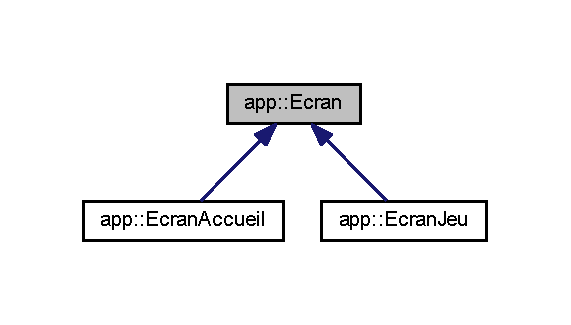
\includegraphics[width=274pt]{classapp_1_1_ecran__inherit__graph}
\end{center}
\end{figure}


Graphe de collaboration de app\+:\+:Ecran\+:\nopagebreak
\begin{figure}[H]
\begin{center}
\leavevmode
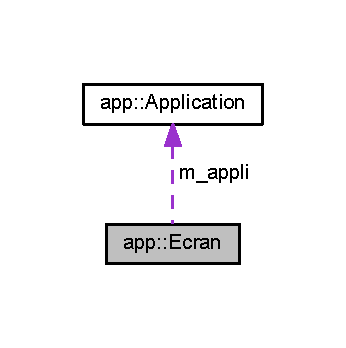
\includegraphics[width=166pt]{classapp_1_1_ecran__coll__graph}
\end{center}
\end{figure}
\subsection*{Fonctions membres publiques}
\begin{DoxyCompactItemize}
\item 
\hyperlink{classapp_1_1_ecran_a06a27f001c26fb8d6f38e04764fd343e}{Ecran} (\hyperlink{classapp_1_1_application}{Application} $\ast$appli)
\begin{DoxyCompactList}\small\item\em Constructeur. \end{DoxyCompactList}\item 
virtual \hyperlink{classapp_1_1_ecran_aee32b1927cc8d449f10c13fd117bcc4a}{$\sim$\+Ecran} ()
\begin{DoxyCompactList}\small\item\em Destructeur virtuel. \end{DoxyCompactList}\item 
virtual void \hyperlink{classapp_1_1_ecran_a15b6695f6950903f11a378759aaa9a23}{traiter\+\_\+evenements} (const sf\+::\+Event \&event)=0
\begin{DoxyCompactList}\small\item\em G�re les entr�es claviers, souris, fenetre ... \end{DoxyCompactList}\item 
virtual void \hyperlink{classapp_1_1_ecran_a209a7aa65901b0d7199c3ca25d7e5794}{actualiser} (sf\+::\+Time deltaT)=0
\begin{DoxyCompactList}\small\item\em Actualiser les �l�ments. \end{DoxyCompactList}\item 
virtual void \hyperlink{classapp_1_1_ecran_ab279679638e35645bbae78e3f8a3938a}{dessiner} ()=0
\begin{DoxyCompactList}\small\item\em Rendre les �l�ments. \end{DoxyCompactList}\end{DoxyCompactItemize}
\subsection*{Attributs protégés}
\begin{DoxyCompactItemize}
\item 
\hyperlink{classapp_1_1_application}{Application} $\ast$ \hyperlink{classapp_1_1_ecran_a4711fc3fedd9458041b1f15b2f05f1a1}{m\+\_\+appli}
\begin{DoxyCompactList}\small\item\em La classe Apllication parent. \end{DoxyCompactList}\item 
sf\+::\+View \hyperlink{classapp_1_1_ecran_aa619321cb264726990dc6a4362876db1}{m\+\_\+vue\+Jeu}
\item 
sf\+::\+View \hyperlink{classapp_1_1_ecran_a5ec228de93b9a07954be2e25371cd9db}{m\+\_\+vue\+G\+UI}
\end{DoxyCompactItemize}


\subsection{Description détaillée}
La classe virtuelle communues aux �crans. 

\hyperlink{classapp_1_1_ecran}{app\+::\+Ecran} la classe de base des �crans. Les �crans peuvent se superposer (par exemple l\textquotesingle{}�cran pause-\/option avec en dessous l\textquotesingle{}�cran jeu en pause).

\begin{DoxySeeAlso}{Voir également}
app\+::\+Ecran\+Demo 
\end{DoxySeeAlso}


\subsection{Documentation des constructeurs et destructeur}
\index{app\+::\+Ecran@{app\+::\+Ecran}!Ecran@{Ecran}}
\index{Ecran@{Ecran}!app\+::\+Ecran@{app\+::\+Ecran}}
\subsubsection[{\texorpdfstring{Ecran(\+Application $\ast$appli)}{Ecran(Application *appli)}}]{\setlength{\rightskip}{0pt plus 5cm}app\+::\+Ecran\+::\+Ecran (
\begin{DoxyParamCaption}
\item[{{\bf Application} $\ast$}]{appli}
\end{DoxyParamCaption}
)}\hypertarget{classapp_1_1_ecran_a06a27f001c26fb8d6f38e04764fd343e}{}\label{classapp_1_1_ecran_a06a27f001c26fb8d6f38e04764fd343e}


Constructeur. 

\index{app\+::\+Ecran@{app\+::\+Ecran}!````~Ecran@{$\sim$\+Ecran}}
\index{````~Ecran@{$\sim$\+Ecran}!app\+::\+Ecran@{app\+::\+Ecran}}
\subsubsection[{\texorpdfstring{$\sim$\+Ecran()}{~Ecran()}}]{\setlength{\rightskip}{0pt plus 5cm}virtual app\+::\+Ecran\+::$\sim$\+Ecran (
\begin{DoxyParamCaption}
{}
\end{DoxyParamCaption}
)\hspace{0.3cm}{\ttfamily [virtual]}}\hypertarget{classapp_1_1_ecran_aee32b1927cc8d449f10c13fd117bcc4a}{}\label{classapp_1_1_ecran_aee32b1927cc8d449f10c13fd117bcc4a}


Destructeur virtuel. 



\subsection{Documentation des fonctions membres}
\index{app\+::\+Ecran@{app\+::\+Ecran}!actualiser@{actualiser}}
\index{actualiser@{actualiser}!app\+::\+Ecran@{app\+::\+Ecran}}
\subsubsection[{\texorpdfstring{actualiser(sf\+::\+Time delta\+T)=0}{actualiser(sf::Time deltaT)=0}}]{\setlength{\rightskip}{0pt plus 5cm}virtual void app\+::\+Ecran\+::actualiser (
\begin{DoxyParamCaption}
\item[{sf\+::\+Time}]{deltaT}
\end{DoxyParamCaption}
)\hspace{0.3cm}{\ttfamily [pure virtual]}}\hypertarget{classapp_1_1_ecran_a209a7aa65901b0d7199c3ca25d7e5794}{}\label{classapp_1_1_ecran_a209a7aa65901b0d7199c3ca25d7e5794}


Actualiser les �l�ments. 

Actualiser les diff�rents �l�ments du ou des �crans actifs.


\begin{DoxyParams}{Paramètres}
{\em deltaT} & Un {\itshape float} qui indique le delta du temps �coul� depuis la derni�re actualisation. \\
\hline
\end{DoxyParams}
\begin{DoxyReturn}{Renvoie}
Rien 
\end{DoxyReturn}
\index{app\+::\+Ecran@{app\+::\+Ecran}!dessiner@{dessiner}}
\index{dessiner@{dessiner}!app\+::\+Ecran@{app\+::\+Ecran}}
\subsubsection[{\texorpdfstring{dessiner()=0}{dessiner()=0}}]{\setlength{\rightskip}{0pt plus 5cm}virtual void app\+::\+Ecran\+::dessiner (
\begin{DoxyParamCaption}
{}
\end{DoxyParamCaption}
)\hspace{0.3cm}{\ttfamily [pure virtual]}}\hypertarget{classapp_1_1_ecran_ab279679638e35645bbae78e3f8a3938a}{}\label{classapp_1_1_ecran_ab279679638e35645bbae78e3f8a3938a}


Rendre les �l�ments. 

Dessiner les diff�rents �l�ments du ou des �crans actifs. \begin{DoxyReturn}{Renvoie}
Rien 
\end{DoxyReturn}
\index{app\+::\+Ecran@{app\+::\+Ecran}!traiter\+\_\+evenements@{traiter\+\_\+evenements}}
\index{traiter\+\_\+evenements@{traiter\+\_\+evenements}!app\+::\+Ecran@{app\+::\+Ecran}}
\subsubsection[{\texorpdfstring{traiter\+\_\+evenements(const sf\+::\+Event \&event)=0}{traiter_evenements(const sf::Event &event)=0}}]{\setlength{\rightskip}{0pt plus 5cm}virtual void app\+::\+Ecran\+::traiter\+\_\+evenements (
\begin{DoxyParamCaption}
\item[{const sf\+::\+Event \&}]{event}
\end{DoxyParamCaption}
)\hspace{0.3cm}{\ttfamily [pure virtual]}}\hypertarget{classapp_1_1_ecran_a15b6695f6950903f11a378759aaa9a23}{}\label{classapp_1_1_ecran_a15b6695f6950903f11a378759aaa9a23}


G�re les entr�es claviers, souris, fenetre ... 


\begin{DoxyParams}{Paramètres}
{\em event} & evenement S\+F\+ML a dispatcher \\
\hline
\end{DoxyParams}
\begin{DoxyReturn}{Renvoie}
rien 
\end{DoxyReturn}


\subsection{Documentation des données membres}
\index{app\+::\+Ecran@{app\+::\+Ecran}!m\+\_\+appli@{m\+\_\+appli}}
\index{m\+\_\+appli@{m\+\_\+appli}!app\+::\+Ecran@{app\+::\+Ecran}}
\subsubsection[{\texorpdfstring{m\+\_\+appli}{m_appli}}]{\setlength{\rightskip}{0pt plus 5cm}{\bf Application}$\ast$ app\+::\+Ecran\+::m\+\_\+appli\hspace{0.3cm}{\ttfamily [protected]}}\hypertarget{classapp_1_1_ecran_a4711fc3fedd9458041b1f15b2f05f1a1}{}\label{classapp_1_1_ecran_a4711fc3fedd9458041b1f15b2f05f1a1}


La classe Apllication parent. 

\index{app\+::\+Ecran@{app\+::\+Ecran}!m\+\_\+vue\+G\+UI@{m\+\_\+vue\+G\+UI}}
\index{m\+\_\+vue\+G\+UI@{m\+\_\+vue\+G\+UI}!app\+::\+Ecran@{app\+::\+Ecran}}
\subsubsection[{\texorpdfstring{m\+\_\+vue\+G\+UI}{m_vueGUI}}]{\setlength{\rightskip}{0pt plus 5cm}sf\+::\+View app\+::\+Ecran\+::m\+\_\+vue\+G\+UI\hspace{0.3cm}{\ttfamily [protected]}}\hypertarget{classapp_1_1_ecran_a5ec228de93b9a07954be2e25371cd9db}{}\label{classapp_1_1_ecran_a5ec228de93b9a07954be2e25371cd9db}
\index{app\+::\+Ecran@{app\+::\+Ecran}!m\+\_\+vue\+Jeu@{m\+\_\+vue\+Jeu}}
\index{m\+\_\+vue\+Jeu@{m\+\_\+vue\+Jeu}!app\+::\+Ecran@{app\+::\+Ecran}}
\subsubsection[{\texorpdfstring{m\+\_\+vue\+Jeu}{m_vueJeu}}]{\setlength{\rightskip}{0pt plus 5cm}sf\+::\+View app\+::\+Ecran\+::m\+\_\+vue\+Jeu\hspace{0.3cm}{\ttfamily [protected]}}\hypertarget{classapp_1_1_ecran_aa619321cb264726990dc6a4362876db1}{}\label{classapp_1_1_ecran_aa619321cb264726990dc6a4362876db1}


La documentation de cette classe a été générée à partir du fichier suivant \+:\begin{DoxyCompactItemize}
\item 
C\+:/\+Users/kris/\+One\+Drive/recherche Biome/01 -\/ code/code/include/appli/\hyperlink{_ecran_8h}{Ecran.\+h}\end{DoxyCompactItemize}

\hypertarget{classapp_1_1_ecran_accueil}{}\section{Référence de la classe app\+:\+:Ecran\+Accueil}
\label{classapp_1_1_ecran_accueil}\index{app\+::\+Ecran\+Accueil@{app\+::\+Ecran\+Accueil}}


\hyperlink{classapp_1_1_ecran}{Ecran} de démonstration.  




{\ttfamily \#include $<$Ecran\+Accueil.\+h$>$}



Graphe d\textquotesingle{}héritage de app\+:\+:Ecran\+Accueil\+:\nopagebreak
\begin{figure}[H]
\begin{center}
\leavevmode
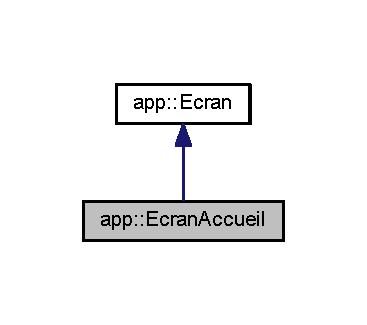
\includegraphics[width=176pt]{classapp_1_1_ecran_accueil__inherit__graph}
\end{center}
\end{figure}


Graphe de collaboration de app\+:\+:Ecran\+Accueil\+:\nopagebreak
\begin{figure}[H]
\begin{center}
\leavevmode
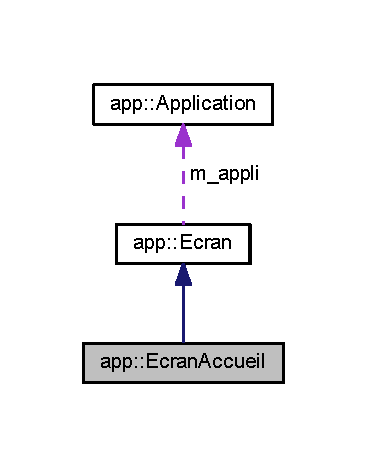
\includegraphics[width=176pt]{classapp_1_1_ecran_accueil__coll__graph}
\end{center}
\end{figure}
\subsection*{Fonctions membres publiques}
\begin{DoxyCompactItemize}
\item 
\hyperlink{classapp_1_1_ecran_accueil_a7b781fae43e45039ea5c0bbf96410cb8}{Ecran\+Accueil} (\hyperlink{classapp_1_1_application}{Application} $\ast$appli)
\begin{DoxyCompactList}\small\item\em Constructeur. \end{DoxyCompactList}\item 
\hyperlink{classapp_1_1_ecran_accueil_a9974fdcf2ef4b88851a8eab56939fcd5}{$\sim$\+Ecran\+Accueil} ()
\begin{DoxyCompactList}\small\item\em Destructeur. \end{DoxyCompactList}\end{DoxyCompactItemize}
\subsection*{Membres hérités additionnels}


\subsection{Description détaillée}
\hyperlink{classapp_1_1_ecran}{Ecran} de démonstration. 

Peut-\/être pour tester d\textquotesingle{}autre trucs, comme la bibilo d\textquotesingle{}interface graphique... 

\subsection{Documentation des constructeurs et destructeur}
\index{app\+::\+Ecran\+Accueil@{app\+::\+Ecran\+Accueil}!Ecran\+Accueil@{Ecran\+Accueil}}
\index{Ecran\+Accueil@{Ecran\+Accueil}!app\+::\+Ecran\+Accueil@{app\+::\+Ecran\+Accueil}}
\subsubsection[{\texorpdfstring{Ecran\+Accueil(\+Application $\ast$appli)}{EcranAccueil(Application *appli)}}]{\setlength{\rightskip}{0pt plus 5cm}app\+::\+Ecran\+Accueil\+::\+Ecran\+Accueil (
\begin{DoxyParamCaption}
\item[{{\bf Application} $\ast$}]{appli}
\end{DoxyParamCaption}
)}\hypertarget{classapp_1_1_ecran_accueil_a7b781fae43e45039ea5c0bbf96410cb8}{}\label{classapp_1_1_ecran_accueil_a7b781fae43e45039ea5c0bbf96410cb8}


Constructeur. 

\index{app\+::\+Ecran\+Accueil@{app\+::\+Ecran\+Accueil}!````~Ecran\+Accueil@{$\sim$\+Ecran\+Accueil}}
\index{````~Ecran\+Accueil@{$\sim$\+Ecran\+Accueil}!app\+::\+Ecran\+Accueil@{app\+::\+Ecran\+Accueil}}
\subsubsection[{\texorpdfstring{$\sim$\+Ecran\+Accueil()}{~EcranAccueil()}}]{\setlength{\rightskip}{0pt plus 5cm}app\+::\+Ecran\+Accueil\+::$\sim$\+Ecran\+Accueil (
\begin{DoxyParamCaption}
{}
\end{DoxyParamCaption}
)}\hypertarget{classapp_1_1_ecran_accueil_a9974fdcf2ef4b88851a8eab56939fcd5}{}\label{classapp_1_1_ecran_accueil_a9974fdcf2ef4b88851a8eab56939fcd5}


Destructeur. 



La documentation de cette classe a été générée à partir du fichier suivant \+:\begin{DoxyCompactItemize}
\item 
C\+:/\+Users/kris/\+One\+Drive/recherche Biome/01 -\/ code/code/include/appli/ecrans/\hyperlink{_ecran_accueil_8h}{Ecran\+Accueil.\+h}\end{DoxyCompactItemize}

\hypertarget{classapp_1_1_ecran_jeu}{}\section{Référence de la classe app\+:\+:Ecran\+Jeu}
\label{classapp_1_1_ecran_jeu}\index{app\+::\+Ecran\+Jeu@{app\+::\+Ecran\+Jeu}}


\hyperlink{classapp_1_1_ecran}{Ecran} de jeu.  




{\ttfamily \#include $<$Ecran\+Jeu.\+h$>$}



Graphe d\textquotesingle{}héritage de app\+:\+:Ecran\+Jeu\+:\nopagebreak
\begin{figure}[H]
\begin{center}
\leavevmode
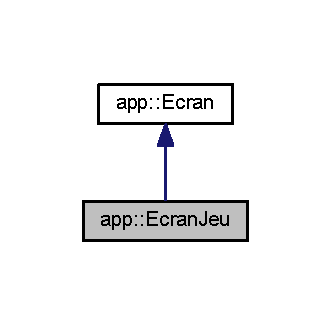
\includegraphics[width=159pt]{classapp_1_1_ecran_jeu__inherit__graph}
\end{center}
\end{figure}


Graphe de collaboration de app\+:\+:Ecran\+Jeu\+:\nopagebreak
\begin{figure}[H]
\begin{center}
\leavevmode
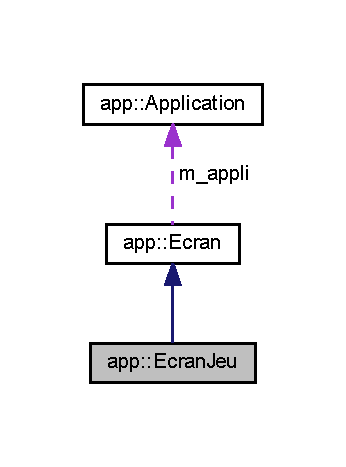
\includegraphics[width=166pt]{classapp_1_1_ecran_jeu__coll__graph}
\end{center}
\end{figure}
\subsection*{Fonctions membres publiques}
\begin{DoxyCompactItemize}
\item 
\hyperlink{classapp_1_1_ecran_jeu_a9c61dc5b68650156f7380fe0739c4622}{Ecran\+Jeu} (\hyperlink{classapp_1_1_application}{Application} $\ast$appli)
\begin{DoxyCompactList}\small\item\em Constructeur. \end{DoxyCompactList}\end{DoxyCompactItemize}
\subsection*{Membres hérités additionnels}


\subsection{Description détaillée}
\hyperlink{classapp_1_1_ecran}{Ecran} de jeu. 

\subsection{Documentation des constructeurs et destructeur}
\index{app\+::\+Ecran\+Jeu@{app\+::\+Ecran\+Jeu}!Ecran\+Jeu@{Ecran\+Jeu}}
\index{Ecran\+Jeu@{Ecran\+Jeu}!app\+::\+Ecran\+Jeu@{app\+::\+Ecran\+Jeu}}
\subsubsection[{\texorpdfstring{Ecran\+Jeu(\+Application $\ast$appli)}{EcranJeu(Application *appli)}}]{\setlength{\rightskip}{0pt plus 5cm}app\+::\+Ecran\+Jeu\+::\+Ecran\+Jeu (
\begin{DoxyParamCaption}
\item[{{\bf Application} $\ast$}]{appli}
\end{DoxyParamCaption}
)}\hypertarget{classapp_1_1_ecran_jeu_a9c61dc5b68650156f7380fe0739c4622}{}\label{classapp_1_1_ecran_jeu_a9c61dc5b68650156f7380fe0739c4622}


Constructeur. 



La documentation de cette classe a été générée à partir du fichier suivant \+:\begin{DoxyCompactItemize}
\item 
C\+:/\+Users/kris/\+One\+Drive/recherche Biome/01 -\/ code/code/include/appli/ecrans/\hyperlink{_ecran_jeu_8h}{Ecran\+Jeu.\+h}\end{DoxyCompactItemize}

\hypertarget{classjeu_1_1_etage}{}\section{Référence de la classe jeu\+:\+:Etage}
\label{classjeu_1_1_etage}\index{jeu\+::\+Etage@{jeu\+::\+Etage}}


Un seul �tage est visible � la fois. Compos� de sol, terre et vide. Chaque �tage g�re les collisions.  




{\ttfamily \#include $<$Etage.\+h$>$}



Graphe d\textquotesingle{}héritage de jeu\+:\+:Etage\+:\nopagebreak
\begin{figure}[H]
\begin{center}
\leavevmode
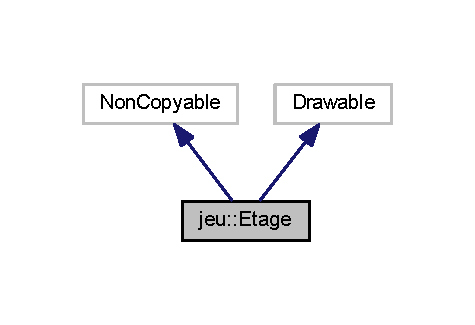
\includegraphics[width=228pt]{classjeu_1_1_etage__inherit__graph}
\end{center}
\end{figure}


Graphe de collaboration de jeu\+:\+:Etage\+:\nopagebreak
\begin{figure}[H]
\begin{center}
\leavevmode
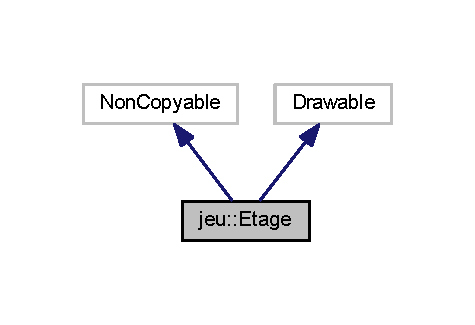
\includegraphics[width=228pt]{classjeu_1_1_etage__coll__graph}
\end{center}
\end{figure}
\subsection*{Fonctions membres publiques}
\begin{DoxyCompactItemize}
\item 
\hyperlink{classjeu_1_1_etage_a66c9cbcd53a3d363b0e539bdbea8f7c8}{Etage} ()
\begin{DoxyCompactList}\small\item\em Constructeur par d�faut. \end{DoxyCompactList}\end{DoxyCompactItemize}


\subsection{Description détaillée}
Un seul �tage est visible � la fois. Compos� de sol, terre et vide. Chaque �tage g�re les collisions. 

\subsection{Documentation des constructeurs et destructeur}
\index{jeu\+::\+Etage@{jeu\+::\+Etage}!Etage@{Etage}}
\index{Etage@{Etage}!jeu\+::\+Etage@{jeu\+::\+Etage}}
\subsubsection[{\texorpdfstring{Etage()}{Etage()}}]{\setlength{\rightskip}{0pt plus 5cm}jeu\+::\+Etage\+::\+Etage (
\begin{DoxyParamCaption}
{}
\end{DoxyParamCaption}
)}\hypertarget{classjeu_1_1_etage_a66c9cbcd53a3d363b0e539bdbea8f7c8}{}\label{classjeu_1_1_etage_a66c9cbcd53a3d363b0e539bdbea8f7c8}


Constructeur par d�faut. 



La documentation de cette classe a été générée à partir du fichier suivant \+:\begin{DoxyCompactItemize}
\item 
C\+:/\+Users/kris/\+One\+Drive/recherche Biome/01 -\/ code/code/include/jeu/\hyperlink{_etage_8h}{Etage.\+h}\end{DoxyCompactItemize}

\hypertarget{classgui_1_1_fabrique}{}\section{Référence de la classe gui\+:\+:Fabrique}
\label{classgui_1_1_fabrique}\index{gui\+::\+Fabrique@{gui\+::\+Fabrique}}


La fabrique des gadget.  




{\ttfamily \#include $<$Fabrique.\+h$>$}

\subsection*{Fonctions membres publiques}
\begin{DoxyCompactItemize}
\item 
std\+::shared\+\_\+ptr$<$ \hyperlink{classgui_1_1_label}{Label} $>$ \hyperlink{classgui_1_1_fabrique_a552610a2e87143c9d2af41ef78fc788a}{label} (string texte)
\begin{DoxyCompactList}\small\item\em Cr�er un label. \end{DoxyCompactList}\end{DoxyCompactItemize}


\subsection{Description détaillée}
La fabrique des gadget. 

\subsection{Documentation des fonctions membres}
\index{gui\+::\+Fabrique@{gui\+::\+Fabrique}!label@{label}}
\index{label@{label}!gui\+::\+Fabrique@{gui\+::\+Fabrique}}
\subsubsection[{\texorpdfstring{label(string texte)}{label(string texte)}}]{\setlength{\rightskip}{0pt plus 5cm}std\+::shared\+\_\+ptr$<${\bf Label}$>$ gui\+::\+Fabrique\+::label (
\begin{DoxyParamCaption}
\item[{string}]{texte}
\end{DoxyParamCaption}
)}\hypertarget{classgui_1_1_fabrique_a552610a2e87143c9d2af41ef78fc788a}{}\label{classgui_1_1_fabrique_a552610a2e87143c9d2af41ef78fc788a}


Cr�er un label. 

\begin{DoxyReturn}{Renvoie}
un pointeur vers le nouveau label cr��.
\end{DoxyReturn}

\begin{DoxyParams}{Paramètres}
{\em texte} & Le texte du label. \\
\hline
\end{DoxyParams}


La documentation de cette classe a été générée à partir du fichier suivant \+:\begin{DoxyCompactItemize}
\item 
C\+:/\+Users/kris/\+One\+Drive/recherche Biome/01 -\/ code/code/include/gui/\hyperlink{_fabrique_8h}{Fabrique.\+h}\end{DoxyCompactItemize}

\hypertarget{classgui_1_1_fenetre}{}\section{Référence de la classe gui\+:\+:Fenetre}
\label{classgui_1_1_fenetre}\index{gui\+::\+Fenetre@{gui\+::\+Fenetre}}


Une fen�tre encapsule des �l�ments d\textquotesingle{}interface.  




{\ttfamily \#include $<$Fenetre.\+h$>$}



Graphe d\textquotesingle{}héritage de gui\+:\+:Fenetre\+:\nopagebreak
\begin{figure}[H]
\begin{center}
\leavevmode
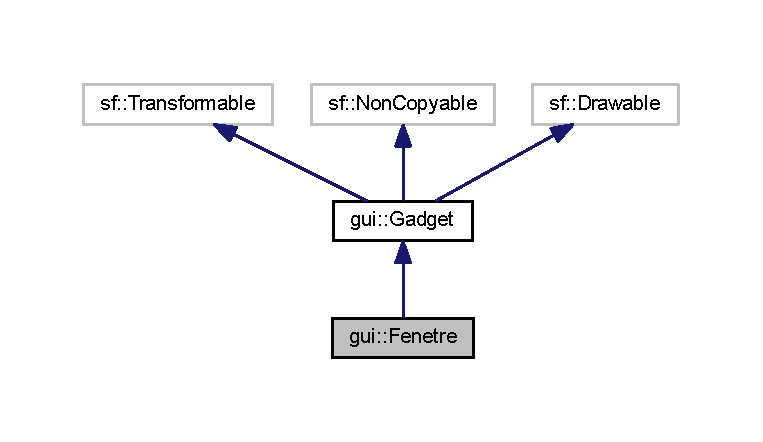
\includegraphics[width=350pt]{classgui_1_1_fenetre__inherit__graph}
\end{center}
\end{figure}


Graphe de collaboration de gui\+:\+:Fenetre\+:\nopagebreak
\begin{figure}[H]
\begin{center}
\leavevmode
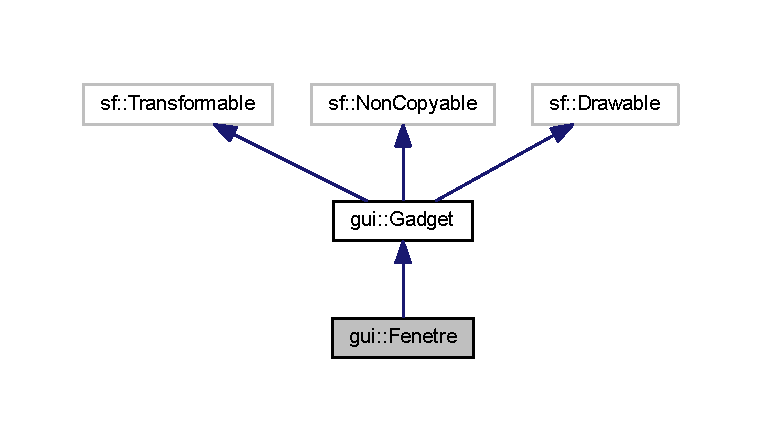
\includegraphics[width=350pt]{classgui_1_1_fenetre__coll__graph}
\end{center}
\end{figure}
\subsection*{Fonctions membres publiques}
\begin{DoxyCompactItemize}
\item 
void \hyperlink{classgui_1_1_fenetre_a997ed9c605a6feecb58f144ef0320540}{traiter\+Evenements} (sf\+::\+Event evenement)
\begin{DoxyCompactList}\small\item\em Traitement des �venements clavier ou souris. \end{DoxyCompactList}\item 
void \hyperlink{classgui_1_1_fenetre_a51255d1ce23986d50ca2a447024a0c14}{actualiser} ()
\begin{DoxyCompactList}\small\item\em Actualiser les �l�ments de l\textquotesingle{}interface. \end{DoxyCompactList}\item 
virtual void \hyperlink{classgui_1_1_fenetre_a189d9d59ab16e81c271414c79eabd8e2}{draw} (sf\+::\+Render\+Target \&target, sf\+::\+Render\+States states) const 
\begin{DoxyCompactList}\small\item\em Dessine tout les �l�ments de l\textquotesingle{}interface. \end{DoxyCompactList}\end{DoxyCompactItemize}


\subsection{Description détaillée}
Une fen�tre encapsule des �l�ments d\textquotesingle{}interface. 

\subsection{Documentation des fonctions membres}
\index{gui\+::\+Fenetre@{gui\+::\+Fenetre}!actualiser@{actualiser}}
\index{actualiser@{actualiser}!gui\+::\+Fenetre@{gui\+::\+Fenetre}}
\subsubsection[{\texorpdfstring{actualiser()}{actualiser()}}]{\setlength{\rightskip}{0pt plus 5cm}void gui\+::\+Fenetre\+::actualiser (
\begin{DoxyParamCaption}
{}
\end{DoxyParamCaption}
)}\hypertarget{classgui_1_1_fenetre_a51255d1ce23986d50ca2a447024a0c14}{}\label{classgui_1_1_fenetre_a51255d1ce23986d50ca2a447024a0c14}


Actualiser les �l�ments de l\textquotesingle{}interface. 

\index{gui\+::\+Fenetre@{gui\+::\+Fenetre}!draw@{draw}}
\index{draw@{draw}!gui\+::\+Fenetre@{gui\+::\+Fenetre}}
\subsubsection[{\texorpdfstring{draw(sf\+::\+Render\+Target \&target, sf\+::\+Render\+States states) const }{draw(sf::RenderTarget &target, sf::RenderStates states) const }}]{\setlength{\rightskip}{0pt plus 5cm}virtual void gui\+::\+Fenetre\+::draw (
\begin{DoxyParamCaption}
\item[{sf\+::\+Render\+Target \&}]{target, }
\item[{sf\+::\+Render\+States}]{states}
\end{DoxyParamCaption}
) const\hspace{0.3cm}{\ttfamily [virtual]}}\hypertarget{classgui_1_1_fenetre_a189d9d59ab16e81c271414c79eabd8e2}{}\label{classgui_1_1_fenetre_a189d9d59ab16e81c271414c79eabd8e2}


Dessine tout les �l�ments de l\textquotesingle{}interface. 


\begin{DoxyParams}{Paramètres}
{\em target} & \\
\hline
{\em states} & \\
\hline
\end{DoxyParams}


Réimplémentée à partir de \hyperlink{classgui_1_1_gadget_a57b0c75601c7f6e0d43370013ae8c111}{gui\+::\+Gadget}.

\index{gui\+::\+Fenetre@{gui\+::\+Fenetre}!traiter\+Evenements@{traiter\+Evenements}}
\index{traiter\+Evenements@{traiter\+Evenements}!gui\+::\+Fenetre@{gui\+::\+Fenetre}}
\subsubsection[{\texorpdfstring{traiter\+Evenements(sf\+::\+Event evenement)}{traiterEvenements(sf::Event evenement)}}]{\setlength{\rightskip}{0pt plus 5cm}void gui\+::\+Fenetre\+::traiter\+Evenements (
\begin{DoxyParamCaption}
\item[{sf\+::\+Event}]{evenement}
\end{DoxyParamCaption}
)}\hypertarget{classgui_1_1_fenetre_a997ed9c605a6feecb58f144ef0320540}{}\label{classgui_1_1_fenetre_a997ed9c605a6feecb58f144ef0320540}


Traitement des �venements clavier ou souris. 


\begin{DoxyParams}{Paramètres}
{\em evenement} & L\textquotesingle{}�venemnt � tratier. \\
\hline
\end{DoxyParams}


La documentation de cette classe a été générée à partir du fichier suivant \+:\begin{DoxyCompactItemize}
\item 
C\+:/\+Users/kris/\+One\+Drive/recherche Biome/01 -\/ code/code/include/gui/\hyperlink{_fenetre_8h}{Fenetre.\+h}\end{DoxyCompactItemize}

\hypertarget{classgui_1_1_gadget}{}\section{Référence de la classe gui\+:\+:Gadget}
\label{classgui_1_1_gadget}\index{gui\+::\+Gadget@{gui\+::\+Gadget}}


Un gadget est la classe abstraite des �l�ments de l\textquotesingle{}interface.  




{\ttfamily \#include $<$Gadget.\+h$>$}



Graphe d\textquotesingle{}héritage de gui\+:\+:Gadget\+:\nopagebreak
\begin{figure}[H]
\begin{center}
\leavevmode
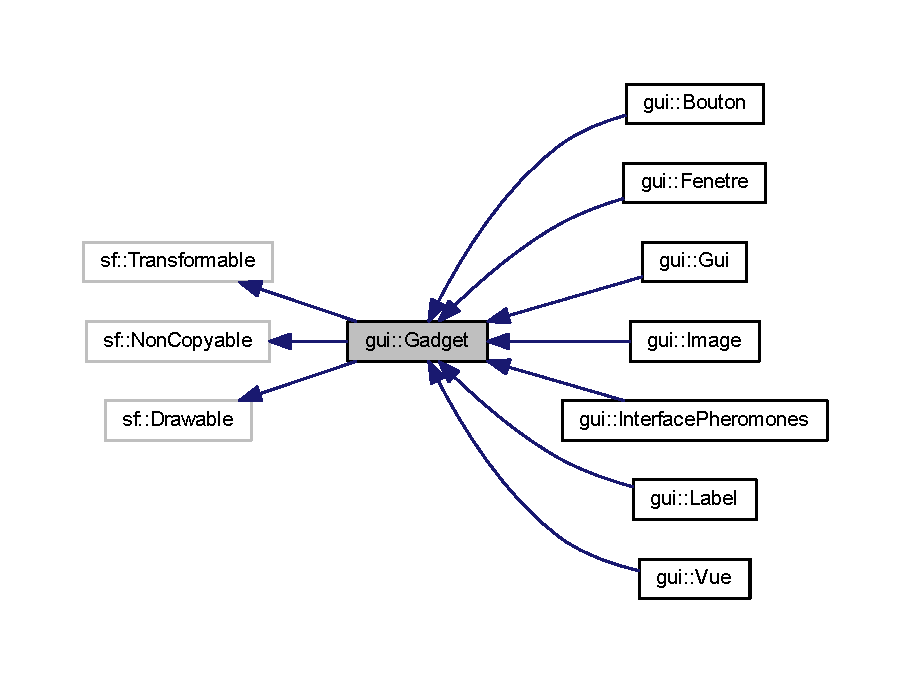
\includegraphics[width=350pt]{classgui_1_1_gadget__inherit__graph}
\end{center}
\end{figure}


Graphe de collaboration de gui\+:\+:Gadget\+:\nopagebreak
\begin{figure}[H]
\begin{center}
\leavevmode
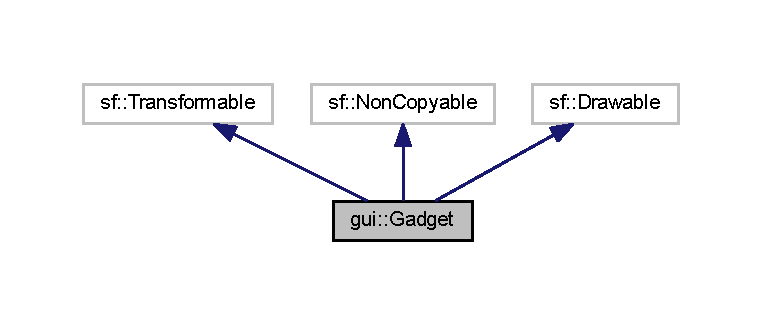
\includegraphics[width=350pt]{classgui_1_1_gadget__coll__graph}
\end{center}
\end{figure}
\subsection*{Fonctions membres publiques}
\begin{DoxyCompactItemize}
\item 
void \hyperlink{classgui_1_1_gadget_abbcab4a09715dc7937f8988d115034f9}{set\+Parent} (\hyperlink{classgui_1_1_gadget}{Gadget} $\ast$val)
\begin{DoxyCompactList}\small\item\em $<$ Definir m\+\_\+parent \end{DoxyCompactList}\item 
\hyperlink{classgui_1_1_gadget}{Gadget} $\ast$ \hyperlink{classgui_1_1_gadget_adaaf9138ae6935aea792c75be9ec2f70}{get\+Parent} () const 
\begin{DoxyCompactList}\small\item\em Acceder � m\+\_\+parent. \end{DoxyCompactList}\item 
void \hyperlink{classgui_1_1_gadget_aff1d84a5d1ea166b99961ccb7eb7f9af}{ajouter\+A\+Enfants} (std\+::shared\+\_\+ptr$<$ \hyperlink{classgui_1_1_gadget}{Gadget} $>$ nouvel\+Element)
\begin{DoxyCompactList}\small\item\em Ajouter un �lement dans m\+\_\+enfants. \end{DoxyCompactList}\item 
void \hyperlink{classgui_1_1_gadget_a0c68857dc183d23be6bb0eb26e15e345}{retirer\+A\+Enfants} (int id)
\begin{DoxyCompactList}\small\item\em retirer l\textquotesingle{}�lement � la position id dans m\+\_\+enfants \end{DoxyCompactList}\item 
void \hyperlink{classgui_1_1_gadget_aaee75cbdc1244dd38c4c1c40c2c7649a}{vider\+Enfants} ()
\begin{DoxyCompactList}\small\item\em Vider m\+\_\+enfants. \end{DoxyCompactList}\item 
std\+::shared\+\_\+ptr$<$ \hyperlink{classgui_1_1_gadget}{Gadget} $>$ \hyperlink{classgui_1_1_gadget_a790c11fc5b6b6647ae01e8fb010c53f1}{get\+Enfants} (int id) const 
\begin{DoxyCompactList}\small\item\em Accesseur � l\textquotesingle{}�l�ment de m\+\_\+enfants d�sign� par un id. \end{DoxyCompactList}\item 
void \hyperlink{classgui_1_1_gadget_aeec07108a3ee71bcbc6d722fcc6f55a9}{set\+Size} (sf\+::\+Vector2i val)
\begin{DoxyCompactList}\small\item\em Definir m\+\_\+size. \end{DoxyCompactList}\item 
sf\+::\+Vector2i \hyperlink{classgui_1_1_gadget_a14394919166b43c08176ea40a494c6c2}{get\+Size} () const 
\begin{DoxyCompactList}\small\item\em Acceder � m\+\_\+size. \end{DoxyCompactList}\item 
sf\+::\+Int\+Rect \hyperlink{classgui_1_1_gadget_af2f1b38002fb1eaf0b31b86b0c3e4401}{get\+Global\+Bounds} () const 
\begin{DoxyCompactList}\small\item\em Acceder � m\+\_\+global\+Bounds. \end{DoxyCompactList}\item 
sf\+::\+Int\+Rect \hyperlink{classgui_1_1_gadget_a9618784a15aedf679d52dfe46d5b6cb7}{get\+Local\+Bounds} () const 
\begin{DoxyCompactList}\small\item\em Acceder � m\+\_\+local\+Bounds. \end{DoxyCompactList}\item 
\hyperlink{classgui_1_1_gadget_a62dfd5bd962b252b792f00b183df9462}{Gadget} ()
\begin{DoxyCompactList}\small\item\em Constructeur. \end{DoxyCompactList}\item 
void \hyperlink{classgui_1_1_gadget_a4425e4e636bbd4f1a3bc548e973ebd20}{traiter\+Evenements} (sf\+::\+Event evenement)
\begin{DoxyCompactList}\small\item\em Traitement des �venements clavier ou souris. \end{DoxyCompactList}\item 
void \hyperlink{classgui_1_1_gadget_aafcfc7ae84fe8277628f971c947b5972}{actualiser} ()
\begin{DoxyCompactList}\small\item\em Actualiser les �l�ments de l\textquotesingle{}interface. \end{DoxyCompactList}\item 
virtual void \hyperlink{classgui_1_1_gadget_a57b0c75601c7f6e0d43370013ae8c111}{draw} (sf\+::\+Render\+Target \&target, sf\+::\+Render\+States states) const 
\begin{DoxyCompactList}\small\item\em Dessine tout les �l�ments de l\textquotesingle{}interface. \end{DoxyCompactList}\item 
virtual std\+::shared\+\_\+ptr$<$ \hyperlink{classgui_1_1_gadget}{Gadget} $>$ \hyperlink{classgui_1_1_gadget_a5768e141631417a5af509da06f7acc9b}{tester\+Survol} () const 
\begin{DoxyCompactList}\small\item\em Teste le survol du gadget par la souris. \end{DoxyCompactList}\end{DoxyCompactItemize}


\subsection{Description détaillée}
Un gadget est la classe abstraite des �l�ments de l\textquotesingle{}interface. 

\subsection{Documentation des constructeurs et destructeur}
\index{gui\+::\+Gadget@{gui\+::\+Gadget}!Gadget@{Gadget}}
\index{Gadget@{Gadget}!gui\+::\+Gadget@{gui\+::\+Gadget}}
\subsubsection[{\texorpdfstring{Gadget()}{Gadget()}}]{\setlength{\rightskip}{0pt plus 5cm}gui\+::\+Gadget\+::\+Gadget (
\begin{DoxyParamCaption}
{}
\end{DoxyParamCaption}
)}\hypertarget{classgui_1_1_gadget_a62dfd5bd962b252b792f00b183df9462}{}\label{classgui_1_1_gadget_a62dfd5bd962b252b792f00b183df9462}


Constructeur. 



\subsection{Documentation des fonctions membres}
\index{gui\+::\+Gadget@{gui\+::\+Gadget}!actualiser@{actualiser}}
\index{actualiser@{actualiser}!gui\+::\+Gadget@{gui\+::\+Gadget}}
\subsubsection[{\texorpdfstring{actualiser()}{actualiser()}}]{\setlength{\rightskip}{0pt plus 5cm}void gui\+::\+Gadget\+::actualiser (
\begin{DoxyParamCaption}
{}
\end{DoxyParamCaption}
)}\hypertarget{classgui_1_1_gadget_aafcfc7ae84fe8277628f971c947b5972}{}\label{classgui_1_1_gadget_aafcfc7ae84fe8277628f971c947b5972}


Actualiser les �l�ments de l\textquotesingle{}interface. 

\index{gui\+::\+Gadget@{gui\+::\+Gadget}!ajouter\+A\+Enfants@{ajouter\+A\+Enfants}}
\index{ajouter\+A\+Enfants@{ajouter\+A\+Enfants}!gui\+::\+Gadget@{gui\+::\+Gadget}}
\subsubsection[{\texorpdfstring{ajouter\+A\+Enfants(std\+::shared\+\_\+ptr$<$ Gadget $>$ nouvel\+Element)}{ajouterAEnfants(std::shared_ptr< Gadget > nouvelElement)}}]{\setlength{\rightskip}{0pt plus 5cm}void gui\+::\+Gadget\+::ajouter\+A\+Enfants (
\begin{DoxyParamCaption}
\item[{std\+::shared\+\_\+ptr$<$ {\bf Gadget} $>$}]{nouvel\+Element}
\end{DoxyParamCaption}
)\hspace{0.3cm}{\ttfamily [inline]}}\hypertarget{classgui_1_1_gadget_aff1d84a5d1ea166b99961ccb7eb7f9af}{}\label{classgui_1_1_gadget_aff1d84a5d1ea166b99961ccb7eb7f9af}


Ajouter un �lement dans m\+\_\+enfants. 

\index{gui\+::\+Gadget@{gui\+::\+Gadget}!draw@{draw}}
\index{draw@{draw}!gui\+::\+Gadget@{gui\+::\+Gadget}}
\subsubsection[{\texorpdfstring{draw(sf\+::\+Render\+Target \&target, sf\+::\+Render\+States states) const }{draw(sf::RenderTarget &target, sf::RenderStates states) const }}]{\setlength{\rightskip}{0pt plus 5cm}virtual void gui\+::\+Gadget\+::draw (
\begin{DoxyParamCaption}
\item[{sf\+::\+Render\+Target \&}]{target, }
\item[{sf\+::\+Render\+States}]{states}
\end{DoxyParamCaption}
) const\hspace{0.3cm}{\ttfamily [virtual]}}\hypertarget{classgui_1_1_gadget_a57b0c75601c7f6e0d43370013ae8c111}{}\label{classgui_1_1_gadget_a57b0c75601c7f6e0d43370013ae8c111}


Dessine tout les �l�ments de l\textquotesingle{}interface. 


\begin{DoxyParams}{Paramètres}
{\em target} & \\
\hline
{\em states} & \\
\hline
\end{DoxyParams}


Réimplémentée dans \hyperlink{classgui_1_1_gui_ab1b62cfabfa4382161f68b4cbbfbd530}{gui\+::\+Gui}, \hyperlink{classgui_1_1_bouton_ae1ae117fb6e67dc7446eeb16c172ea14}{gui\+::\+Bouton}, \hyperlink{classgui_1_1_fenetre_a189d9d59ab16e81c271414c79eabd8e2}{gui\+::\+Fenetre}, \hyperlink{classgui_1_1_image_a6a2948c46b65fcf97646341936ec1aba}{gui\+::\+Image}, \hyperlink{classgui_1_1_interface_pheromones_a970a5c6ef20546ecf0905660c5d0c62a}{gui\+::\+Interface\+Pheromones}, \hyperlink{classgui_1_1_label_a835406d1bc730f86ab715fc70c4541ca}{gui\+::\+Label}, et \hyperlink{classgui_1_1_vue_a1439e18d8ba169399248085867528f26}{gui\+::\+Vue}.

\index{gui\+::\+Gadget@{gui\+::\+Gadget}!get\+Enfants@{get\+Enfants}}
\index{get\+Enfants@{get\+Enfants}!gui\+::\+Gadget@{gui\+::\+Gadget}}
\subsubsection[{\texorpdfstring{get\+Enfants(int id) const }{getEnfants(int id) const }}]{\setlength{\rightskip}{0pt plus 5cm}std\+::shared\+\_\+ptr$<${\bf Gadget}$>$ gui\+::\+Gadget\+::get\+Enfants (
\begin{DoxyParamCaption}
\item[{int}]{id}
\end{DoxyParamCaption}
) const\hspace{0.3cm}{\ttfamily [inline]}}\hypertarget{classgui_1_1_gadget_a790c11fc5b6b6647ae01e8fb010c53f1}{}\label{classgui_1_1_gadget_a790c11fc5b6b6647ae01e8fb010c53f1}


Accesseur � l\textquotesingle{}�l�ment de m\+\_\+enfants d�sign� par un id. 

\index{gui\+::\+Gadget@{gui\+::\+Gadget}!get\+Global\+Bounds@{get\+Global\+Bounds}}
\index{get\+Global\+Bounds@{get\+Global\+Bounds}!gui\+::\+Gadget@{gui\+::\+Gadget}}
\subsubsection[{\texorpdfstring{get\+Global\+Bounds() const }{getGlobalBounds() const }}]{\setlength{\rightskip}{0pt plus 5cm}sf\+::\+Int\+Rect gui\+::\+Gadget\+::get\+Global\+Bounds (
\begin{DoxyParamCaption}
{}
\end{DoxyParamCaption}
) const\hspace{0.3cm}{\ttfamily [inline]}}\hypertarget{classgui_1_1_gadget_af2f1b38002fb1eaf0b31b86b0c3e4401}{}\label{classgui_1_1_gadget_af2f1b38002fb1eaf0b31b86b0c3e4401}


Acceder � m\+\_\+global\+Bounds. 

\index{gui\+::\+Gadget@{gui\+::\+Gadget}!get\+Local\+Bounds@{get\+Local\+Bounds}}
\index{get\+Local\+Bounds@{get\+Local\+Bounds}!gui\+::\+Gadget@{gui\+::\+Gadget}}
\subsubsection[{\texorpdfstring{get\+Local\+Bounds() const }{getLocalBounds() const }}]{\setlength{\rightskip}{0pt plus 5cm}sf\+::\+Int\+Rect gui\+::\+Gadget\+::get\+Local\+Bounds (
\begin{DoxyParamCaption}
{}
\end{DoxyParamCaption}
) const\hspace{0.3cm}{\ttfamily [inline]}}\hypertarget{classgui_1_1_gadget_a9618784a15aedf679d52dfe46d5b6cb7}{}\label{classgui_1_1_gadget_a9618784a15aedf679d52dfe46d5b6cb7}


Acceder � m\+\_\+local\+Bounds. 

\index{gui\+::\+Gadget@{gui\+::\+Gadget}!get\+Parent@{get\+Parent}}
\index{get\+Parent@{get\+Parent}!gui\+::\+Gadget@{gui\+::\+Gadget}}
\subsubsection[{\texorpdfstring{get\+Parent() const }{getParent() const }}]{\setlength{\rightskip}{0pt plus 5cm}{\bf Gadget}$\ast$ gui\+::\+Gadget\+::get\+Parent (
\begin{DoxyParamCaption}
{}
\end{DoxyParamCaption}
) const\hspace{0.3cm}{\ttfamily [inline]}}\hypertarget{classgui_1_1_gadget_adaaf9138ae6935aea792c75be9ec2f70}{}\label{classgui_1_1_gadget_adaaf9138ae6935aea792c75be9ec2f70}


Acceder � m\+\_\+parent. 

\index{gui\+::\+Gadget@{gui\+::\+Gadget}!get\+Size@{get\+Size}}
\index{get\+Size@{get\+Size}!gui\+::\+Gadget@{gui\+::\+Gadget}}
\subsubsection[{\texorpdfstring{get\+Size() const }{getSize() const }}]{\setlength{\rightskip}{0pt plus 5cm}sf\+::\+Vector2i gui\+::\+Gadget\+::get\+Size (
\begin{DoxyParamCaption}
{}
\end{DoxyParamCaption}
) const\hspace{0.3cm}{\ttfamily [inline]}}\hypertarget{classgui_1_1_gadget_a14394919166b43c08176ea40a494c6c2}{}\label{classgui_1_1_gadget_a14394919166b43c08176ea40a494c6c2}


Acceder � m\+\_\+size. 

\index{gui\+::\+Gadget@{gui\+::\+Gadget}!retirer\+A\+Enfants@{retirer\+A\+Enfants}}
\index{retirer\+A\+Enfants@{retirer\+A\+Enfants}!gui\+::\+Gadget@{gui\+::\+Gadget}}
\subsubsection[{\texorpdfstring{retirer\+A\+Enfants(int id)}{retirerAEnfants(int id)}}]{\setlength{\rightskip}{0pt plus 5cm}void gui\+::\+Gadget\+::retirer\+A\+Enfants (
\begin{DoxyParamCaption}
\item[{int}]{id}
\end{DoxyParamCaption}
)\hspace{0.3cm}{\ttfamily [inline]}}\hypertarget{classgui_1_1_gadget_a0c68857dc183d23be6bb0eb26e15e345}{}\label{classgui_1_1_gadget_a0c68857dc183d23be6bb0eb26e15e345}


retirer l\textquotesingle{}�lement � la position id dans m\+\_\+enfants 

\index{gui\+::\+Gadget@{gui\+::\+Gadget}!set\+Parent@{set\+Parent}}
\index{set\+Parent@{set\+Parent}!gui\+::\+Gadget@{gui\+::\+Gadget}}
\subsubsection[{\texorpdfstring{set\+Parent(\+Gadget $\ast$val)}{setParent(Gadget *val)}}]{\setlength{\rightskip}{0pt plus 5cm}void gui\+::\+Gadget\+::set\+Parent (
\begin{DoxyParamCaption}
\item[{{\bf Gadget} $\ast$}]{val}
\end{DoxyParamCaption}
)\hspace{0.3cm}{\ttfamily [inline]}}\hypertarget{classgui_1_1_gadget_abbcab4a09715dc7937f8988d115034f9}{}\label{classgui_1_1_gadget_abbcab4a09715dc7937f8988d115034f9}


$<$ Definir m\+\_\+parent 

\index{gui\+::\+Gadget@{gui\+::\+Gadget}!set\+Size@{set\+Size}}
\index{set\+Size@{set\+Size}!gui\+::\+Gadget@{gui\+::\+Gadget}}
\subsubsection[{\texorpdfstring{set\+Size(sf\+::\+Vector2i val)}{setSize(sf::Vector2i val)}}]{\setlength{\rightskip}{0pt plus 5cm}void gui\+::\+Gadget\+::set\+Size (
\begin{DoxyParamCaption}
\item[{sf\+::\+Vector2i}]{val}
\end{DoxyParamCaption}
)\hspace{0.3cm}{\ttfamily [inline]}}\hypertarget{classgui_1_1_gadget_aeec07108a3ee71bcbc6d722fcc6f55a9}{}\label{classgui_1_1_gadget_aeec07108a3ee71bcbc6d722fcc6f55a9}


Definir m\+\_\+size. 

\index{gui\+::\+Gadget@{gui\+::\+Gadget}!tester\+Survol@{tester\+Survol}}
\index{tester\+Survol@{tester\+Survol}!gui\+::\+Gadget@{gui\+::\+Gadget}}
\subsubsection[{\texorpdfstring{tester\+Survol() const }{testerSurvol() const }}]{\setlength{\rightskip}{0pt plus 5cm}virtual std\+::shared\+\_\+ptr$<${\bf Gadget}$>$ gui\+::\+Gadget\+::tester\+Survol (
\begin{DoxyParamCaption}
{}
\end{DoxyParamCaption}
) const\hspace{0.3cm}{\ttfamily [virtual]}}\hypertarget{classgui_1_1_gadget_a5768e141631417a5af509da06f7acc9b}{}\label{classgui_1_1_gadget_a5768e141631417a5af509da06f7acc9b}


Teste le survol du gadget par la souris. 

\begin{DoxyReturn}{Renvoie}
le gadget survol�, celui si ou un de ses enfants. nullptr si ne survol rien d\textquotesingle{}interactif. 
\end{DoxyReturn}
\index{gui\+::\+Gadget@{gui\+::\+Gadget}!traiter\+Evenements@{traiter\+Evenements}}
\index{traiter\+Evenements@{traiter\+Evenements}!gui\+::\+Gadget@{gui\+::\+Gadget}}
\subsubsection[{\texorpdfstring{traiter\+Evenements(sf\+::\+Event evenement)}{traiterEvenements(sf::Event evenement)}}]{\setlength{\rightskip}{0pt plus 5cm}void gui\+::\+Gadget\+::traiter\+Evenements (
\begin{DoxyParamCaption}
\item[{sf\+::\+Event}]{evenement}
\end{DoxyParamCaption}
)}\hypertarget{classgui_1_1_gadget_a4425e4e636bbd4f1a3bc548e973ebd20}{}\label{classgui_1_1_gadget_a4425e4e636bbd4f1a3bc548e973ebd20}


Traitement des �venements clavier ou souris. 


\begin{DoxyParams}{Paramètres}
{\em evenement} & L\textquotesingle{}�venemnt � tratier. \\
\hline
\end{DoxyParams}
\index{gui\+::\+Gadget@{gui\+::\+Gadget}!vider\+Enfants@{vider\+Enfants}}
\index{vider\+Enfants@{vider\+Enfants}!gui\+::\+Gadget@{gui\+::\+Gadget}}
\subsubsection[{\texorpdfstring{vider\+Enfants()}{viderEnfants()}}]{\setlength{\rightskip}{0pt plus 5cm}void gui\+::\+Gadget\+::vider\+Enfants (
\begin{DoxyParamCaption}
{}
\end{DoxyParamCaption}
)\hspace{0.3cm}{\ttfamily [inline]}}\hypertarget{classgui_1_1_gadget_aaee75cbdc1244dd38c4c1c40c2c7649a}{}\label{classgui_1_1_gadget_aaee75cbdc1244dd38c4c1c40c2c7649a}


Vider m\+\_\+enfants. 



La documentation de cette classe a été générée à partir du fichier suivant \+:\begin{DoxyCompactItemize}
\item 
C\+:/\+Users/kris/\+One\+Drive/recherche Biome/01 -\/ code/code/include/gui/\hyperlink{_gadget_8h}{Gadget.\+h}\end{DoxyCompactItemize}

\hypertarget{classapp_1_1_gestion__ecrans}{}\section{Référence de la classe app\+:\+:Gestion\+\_\+ecrans}
\label{classapp_1_1_gestion__ecrans}\index{app\+::\+Gestion\+\_\+ecrans@{app\+::\+Gestion\+\_\+ecrans}}


Gestionnaire des �crans.  




{\ttfamily \#include $<$Gestion\+\_\+ecrans.\+h$>$}

\subsection*{Fonctions membres publiques}
\begin{DoxyCompactItemize}
\item 
void \hyperlink{classapp_1_1_gestion__ecrans_a576182f13e96e890e961dd1f7f69747b}{ajouter} (\hyperlink{classapp_1_1_ecran}{Ecran} $\ast$ecran)
\begin{DoxyCompactList}\small\item\em Ajouter un �cran sur la pile. \end{DoxyCompactList}\item 
void \hyperlink{classapp_1_1_gestion__ecrans_a0db2b08457f77a9d01ed007d410d2e0c}{retirer} ()
\begin{DoxyCompactList}\small\item\em Retirer l\textquotesingle{}�cran du dessus de la pile. \end{DoxyCompactList}\item 
void \hyperlink{classapp_1_1_gestion__ecrans_a1c7fab33cf6489b092a482bae4b266f7}{vider} ()
\begin{DoxyCompactList}\small\item\em Retirer tout les �crans de la pile. \end{DoxyCompactList}\item 
bool \hyperlink{classapp_1_1_gestion__ecrans_a7424aab98a8b01f5b5e201ee77bbb7bb}{est\+Vide} ()
\begin{DoxyCompactList}\small\item\em Demande si il y a encore des ecrans dans la pile. \end{DoxyCompactList}\item 
void \hyperlink{classapp_1_1_gestion__ecrans_addd582c82b53c7c142d23dbee83c5bbd}{changer} (\hyperlink{classapp_1_1_ecran}{Ecran} $\ast$ecran)
\begin{DoxyCompactList}\small\item\em Changer d\textquotesingle{}�cran. \end{DoxyCompactList}\item 
\hyperlink{classapp_1_1_ecran}{Ecran} $\ast$ \hyperlink{classapp_1_1_gestion__ecrans_ae6e4040862cce8d816a9f771424de11d}{courant} ()
\begin{DoxyCompactList}\small\item\em Renvoie l\textquotesingle{}�cran courant, celui au top de la {\itshape \+\_\+pile}. \end{DoxyCompactList}\item 
void \hyperlink{classapp_1_1_gestion__ecrans_afdca6c8f031948a5ce80136209924fe8}{traiter\+\_\+evenements} (sf\+::\+Event event)
\begin{DoxyCompactList}\small\item\em G�re les �venements des �crans actifs. \end{DoxyCompactList}\item 
void \hyperlink{classapp_1_1_gestion__ecrans_ac271e2ce11691a51f82f54a7c395d565}{actualiser} (sf\+::\+Time deltaT)
\begin{DoxyCompactList}\small\item\em Actualiser les �l�ments. \end{DoxyCompactList}\item 
void \hyperlink{classapp_1_1_gestion__ecrans_a3c413e7ecbcb252c343136465f5be100}{dessiner} ()
\begin{DoxyCompactList}\small\item\em Rendre les �crans de la pile. \end{DoxyCompactList}\end{DoxyCompactItemize}


\subsection{Description détaillée}
Gestionnaire des �crans. 

G�re les diff�rents �crans de l\textquotesingle{}application. C\textquotesingle{}est lui qui porte les �crans actifs du programme. qui permet de passer d\textquotesingle{}un �cran � l\textquotesingle{}autre, etc. \begin{DoxySeeAlso}{Voir également}
\hyperlink{classapp_1_1_ecran}{app\+::\+Ecran} 
\end{DoxySeeAlso}


\subsection{Documentation des fonctions membres}
\index{app\+::\+Gestion\+\_\+ecrans@{app\+::\+Gestion\+\_\+ecrans}!actualiser@{actualiser}}
\index{actualiser@{actualiser}!app\+::\+Gestion\+\_\+ecrans@{app\+::\+Gestion\+\_\+ecrans}}
\subsubsection[{\texorpdfstring{actualiser(sf\+::\+Time delta\+T)}{actualiser(sf::Time deltaT)}}]{\setlength{\rightskip}{0pt plus 5cm}void app\+::\+Gestion\+\_\+ecrans\+::actualiser (
\begin{DoxyParamCaption}
\item[{sf\+::\+Time}]{deltaT}
\end{DoxyParamCaption}
)}\hypertarget{classapp_1_1_gestion__ecrans_ac271e2ce11691a51f82f54a7c395d565}{}\label{classapp_1_1_gestion__ecrans_ac271e2ce11691a51f82f54a7c395d565}


Actualiser les �l�ments. 

Actualiser les diff�rents �l�ments du ou des �crans actifs. 
\begin{DoxyParams}{Paramètres}
{\em deltaT} & Un {\itshape float} qui indique le delta du temps �coul� depuis la derni�re actualisation. \\
\hline
\end{DoxyParams}
\begin{DoxyReturn}{Renvoie}
Rien 
\end{DoxyReturn}
\index{app\+::\+Gestion\+\_\+ecrans@{app\+::\+Gestion\+\_\+ecrans}!ajouter@{ajouter}}
\index{ajouter@{ajouter}!app\+::\+Gestion\+\_\+ecrans@{app\+::\+Gestion\+\_\+ecrans}}
\subsubsection[{\texorpdfstring{ajouter(\+Ecran $\ast$ecran)}{ajouter(Ecran *ecran)}}]{\setlength{\rightskip}{0pt plus 5cm}void app\+::\+Gestion\+\_\+ecrans\+::ajouter (
\begin{DoxyParamCaption}
\item[{{\bf Ecran} $\ast$}]{ecran}
\end{DoxyParamCaption}
)}\hypertarget{classapp_1_1_gestion__ecrans_a576182f13e96e890e961dd1f7f69747b}{}\label{classapp_1_1_gestion__ecrans_a576182f13e96e890e961dd1f7f69747b}


Ajouter un �cran sur la pile. 


\begin{DoxyParams}{Paramètres}
{\em ecran} & Un nouvel {\itshape \hyperlink{classapp_1_1_ecran}{Ecran}} � ajouter � la pile active. \\
\hline
\end{DoxyParams}
\begin{DoxyReturn}{Renvoie}
Rien. 
\end{DoxyReturn}
\index{app\+::\+Gestion\+\_\+ecrans@{app\+::\+Gestion\+\_\+ecrans}!changer@{changer}}
\index{changer@{changer}!app\+::\+Gestion\+\_\+ecrans@{app\+::\+Gestion\+\_\+ecrans}}
\subsubsection[{\texorpdfstring{changer(\+Ecran $\ast$ecran)}{changer(Ecran *ecran)}}]{\setlength{\rightskip}{0pt plus 5cm}void app\+::\+Gestion\+\_\+ecrans\+::changer (
\begin{DoxyParamCaption}
\item[{{\bf Ecran} $\ast$}]{ecran}
\end{DoxyParamCaption}
)}\hypertarget{classapp_1_1_gestion__ecrans_addd582c82b53c7c142d23dbee83c5bbd}{}\label{classapp_1_1_gestion__ecrans_addd582c82b53c7c142d23dbee83c5bbd}


Changer d\textquotesingle{}�cran. 

On retire l\textquotesingle{}�cran en cours, puis on ajoute le nouveau.


\begin{DoxyParams}{Paramètres}
{\em ecran} & le nouvel {\itshape \hyperlink{classapp_1_1_ecran}{Ecran}} � mettre � la place du dernier de la pile. \\
\hline
\end{DoxyParams}
\begin{DoxyReturn}{Renvoie}
Rien 
\end{DoxyReturn}
\index{app\+::\+Gestion\+\_\+ecrans@{app\+::\+Gestion\+\_\+ecrans}!courant@{courant}}
\index{courant@{courant}!app\+::\+Gestion\+\_\+ecrans@{app\+::\+Gestion\+\_\+ecrans}}
\subsubsection[{\texorpdfstring{courant()}{courant()}}]{\setlength{\rightskip}{0pt plus 5cm}{\bf Ecran}$\ast$ app\+::\+Gestion\+\_\+ecrans\+::courant (
\begin{DoxyParamCaption}
{}
\end{DoxyParamCaption}
)}\hypertarget{classapp_1_1_gestion__ecrans_ae6e4040862cce8d816a9f771424de11d}{}\label{classapp_1_1_gestion__ecrans_ae6e4040862cce8d816a9f771424de11d}


Renvoie l\textquotesingle{}�cran courant, celui au top de la {\itshape \+\_\+pile}. 

\begin{DoxyReturn}{Renvoie}
L\textquotesingle{}�cran courant. 
\end{DoxyReturn}
\index{app\+::\+Gestion\+\_\+ecrans@{app\+::\+Gestion\+\_\+ecrans}!dessiner@{dessiner}}
\index{dessiner@{dessiner}!app\+::\+Gestion\+\_\+ecrans@{app\+::\+Gestion\+\_\+ecrans}}
\subsubsection[{\texorpdfstring{dessiner()}{dessiner()}}]{\setlength{\rightskip}{0pt plus 5cm}void app\+::\+Gestion\+\_\+ecrans\+::dessiner (
\begin{DoxyParamCaption}
{}
\end{DoxyParamCaption}
)}\hypertarget{classapp_1_1_gestion__ecrans_a3c413e7ecbcb252c343136465f5be100}{}\label{classapp_1_1_gestion__ecrans_a3c413e7ecbcb252c343136465f5be100}


Rendre les �crans de la pile. 

Dessine les diff�rents �l�ments du ou des �crans de la pile.

\begin{DoxyReturn}{Renvoie}
Rien 
\end{DoxyReturn}
\index{app\+::\+Gestion\+\_\+ecrans@{app\+::\+Gestion\+\_\+ecrans}!est\+Vide@{est\+Vide}}
\index{est\+Vide@{est\+Vide}!app\+::\+Gestion\+\_\+ecrans@{app\+::\+Gestion\+\_\+ecrans}}
\subsubsection[{\texorpdfstring{est\+Vide()}{estVide()}}]{\setlength{\rightskip}{0pt plus 5cm}bool app\+::\+Gestion\+\_\+ecrans\+::est\+Vide (
\begin{DoxyParamCaption}
{}
\end{DoxyParamCaption}
)}\hypertarget{classapp_1_1_gestion__ecrans_a7424aab98a8b01f5b5e201ee77bbb7bb}{}\label{classapp_1_1_gestion__ecrans_a7424aab98a8b01f5b5e201ee77bbb7bb}


Demande si il y a encore des ecrans dans la pile. 

\begin{DoxyReturn}{Renvoie}
bool true si vide. 
\end{DoxyReturn}
\index{app\+::\+Gestion\+\_\+ecrans@{app\+::\+Gestion\+\_\+ecrans}!retirer@{retirer}}
\index{retirer@{retirer}!app\+::\+Gestion\+\_\+ecrans@{app\+::\+Gestion\+\_\+ecrans}}
\subsubsection[{\texorpdfstring{retirer()}{retirer()}}]{\setlength{\rightskip}{0pt plus 5cm}void app\+::\+Gestion\+\_\+ecrans\+::retirer (
\begin{DoxyParamCaption}
{}
\end{DoxyParamCaption}
)}\hypertarget{classapp_1_1_gestion__ecrans_a0db2b08457f77a9d01ed007d410d2e0c}{}\label{classapp_1_1_gestion__ecrans_a0db2b08457f77a9d01ed007d410d2e0c}


Retirer l\textquotesingle{}�cran du dessus de la pile. 

\begin{DoxyReturn}{Renvoie}
Rien. 
\end{DoxyReturn}
\index{app\+::\+Gestion\+\_\+ecrans@{app\+::\+Gestion\+\_\+ecrans}!traiter\+\_\+evenements@{traiter\+\_\+evenements}}
\index{traiter\+\_\+evenements@{traiter\+\_\+evenements}!app\+::\+Gestion\+\_\+ecrans@{app\+::\+Gestion\+\_\+ecrans}}
\subsubsection[{\texorpdfstring{traiter\+\_\+evenements(sf\+::\+Event event)}{traiter_evenements(sf::Event event)}}]{\setlength{\rightskip}{0pt plus 5cm}void app\+::\+Gestion\+\_\+ecrans\+::traiter\+\_\+evenements (
\begin{DoxyParamCaption}
\item[{sf\+::\+Event}]{event}
\end{DoxyParamCaption}
)}\hypertarget{classapp_1_1_gestion__ecrans_afdca6c8f031948a5ce80136209924fe8}{}\label{classapp_1_1_gestion__ecrans_afdca6c8f031948a5ce80136209924fe8}


G�re les �venements des �crans actifs. 

\begin{DoxyReturn}{Renvoie}
Rien 
\end{DoxyReturn}
\index{app\+::\+Gestion\+\_\+ecrans@{app\+::\+Gestion\+\_\+ecrans}!vider@{vider}}
\index{vider@{vider}!app\+::\+Gestion\+\_\+ecrans@{app\+::\+Gestion\+\_\+ecrans}}
\subsubsection[{\texorpdfstring{vider()}{vider()}}]{\setlength{\rightskip}{0pt plus 5cm}void app\+::\+Gestion\+\_\+ecrans\+::vider (
\begin{DoxyParamCaption}
{}
\end{DoxyParamCaption}
)}\hypertarget{classapp_1_1_gestion__ecrans_a1c7fab33cf6489b092a482bae4b266f7}{}\label{classapp_1_1_gestion__ecrans_a1c7fab33cf6489b092a482bae4b266f7}


Retirer tout les �crans de la pile. 

\begin{DoxyReturn}{Renvoie}
Rien. 
\end{DoxyReturn}


La documentation de cette classe a été générée à partir du fichier suivant \+:\begin{DoxyCompactItemize}
\item 
C\+:/\+Users/kris/\+One\+Drive/recherche Biome/01 -\/ code/code/include/appli/\hyperlink{_gestion__ecrans_8h}{Gestion\+\_\+ecrans.\+h}\end{DoxyCompactItemize}

\hypertarget{classgui_1_1_gui}{}\section{Référence de la classe gui\+:\+:Gui}
\label{classgui_1_1_gui}\index{gui\+::\+Gui@{gui\+::\+Gui}}


Le \hyperlink{classgui_1_1_gui}{Gui} g�re l\textquotesingle{}ensemble des interactions homme-\/machine du jeu. D\textquotesingle{}un cot� un syst�me de fen�tre, boutons basique g�rant les diff�rents menus de l\textquotesingle{}appli. De l\textquotesingle{}autre, le menu ph�romones, syst�me central de l\textquotesingle{}interaction du joueur avec ses fourmis.  




{\ttfamily \#include $<$Gui.\+h$>$}



Graphe d\textquotesingle{}héritage de gui\+:\+:Gui\+:\nopagebreak
\begin{figure}[H]
\begin{center}
\leavevmode
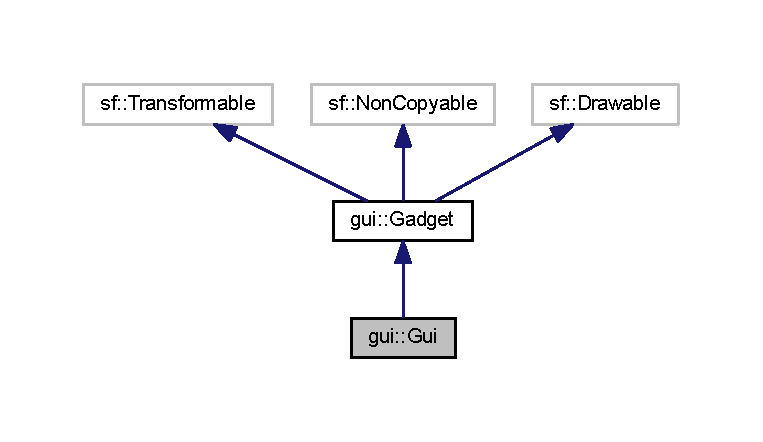
\includegraphics[width=350pt]{classgui_1_1_gui__inherit__graph}
\end{center}
\end{figure}


Graphe de collaboration de gui\+:\+:Gui\+:\nopagebreak
\begin{figure}[H]
\begin{center}
\leavevmode
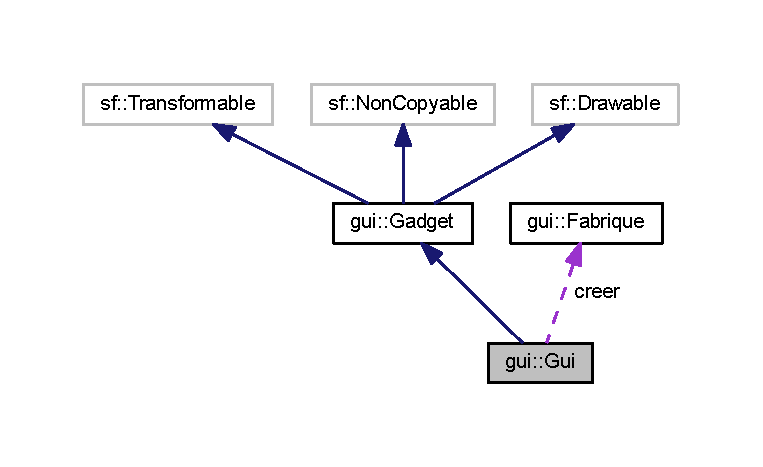
\includegraphics[width=350pt]{classgui_1_1_gui__coll__graph}
\end{center}
\end{figure}
\subsection*{Fonctions membres publiques}
\begin{DoxyCompactItemize}
\item 
void \hyperlink{classgui_1_1_gui_a6e0209d60ac47f2c86e8340a9b4a64b1}{traiter\+Evenements} (sf\+::\+Event evenement)
\begin{DoxyCompactList}\small\item\em Traitement des �venements clavier ou souris. \end{DoxyCompactList}\item 
void \hyperlink{classgui_1_1_gui_ad10b5a8ef07513c03c9126a3eef9955b}{actualiser} ()
\begin{DoxyCompactList}\small\item\em Actualiser les �l�ments de l\textquotesingle{}interface. \end{DoxyCompactList}\item 
virtual void \hyperlink{classgui_1_1_gui_ab1b62cfabfa4382161f68b4cbbfbd530}{draw} (sf\+::\+Render\+Target \&target, sf\+::\+Render\+States states) const 
\begin{DoxyCompactList}\small\item\em Dessine tout les �l�ments de l\textquotesingle{}interface. \end{DoxyCompactList}\end{DoxyCompactItemize}
\subsection*{Attributs publics}
\begin{DoxyCompactItemize}
\item 
\hyperlink{classgui_1_1_fabrique}{gui\+::\+Fabrique} \hyperlink{classgui_1_1_gui_ae5dd6ef6163bce1ef69086bd7dd0c49b}{creer}
\begin{DoxyCompactList}\small\item\em La fabrique des gadget. \end{DoxyCompactList}\end{DoxyCompactItemize}


\subsection{Description détaillée}
Le \hyperlink{classgui_1_1_gui}{Gui} g�re l\textquotesingle{}ensemble des interactions homme-\/machine du jeu. D\textquotesingle{}un cot� un syst�me de fen�tre, boutons basique g�rant les diff�rents menus de l\textquotesingle{}appli. De l\textquotesingle{}autre, le menu ph�romones, syst�me central de l\textquotesingle{}interaction du joueur avec ses fourmis. 

\subsection{Documentation des fonctions membres}
\index{gui\+::\+Gui@{gui\+::\+Gui}!actualiser@{actualiser}}
\index{actualiser@{actualiser}!gui\+::\+Gui@{gui\+::\+Gui}}
\subsubsection[{\texorpdfstring{actualiser()}{actualiser()}}]{\setlength{\rightskip}{0pt plus 5cm}void gui\+::\+Gui\+::actualiser (
\begin{DoxyParamCaption}
{}
\end{DoxyParamCaption}
)}\hypertarget{classgui_1_1_gui_ad10b5a8ef07513c03c9126a3eef9955b}{}\label{classgui_1_1_gui_ad10b5a8ef07513c03c9126a3eef9955b}


Actualiser les �l�ments de l\textquotesingle{}interface. 

\index{gui\+::\+Gui@{gui\+::\+Gui}!draw@{draw}}
\index{draw@{draw}!gui\+::\+Gui@{gui\+::\+Gui}}
\subsubsection[{\texorpdfstring{draw(sf\+::\+Render\+Target \&target, sf\+::\+Render\+States states) const }{draw(sf::RenderTarget &target, sf::RenderStates states) const }}]{\setlength{\rightskip}{0pt plus 5cm}virtual void gui\+::\+Gui\+::draw (
\begin{DoxyParamCaption}
\item[{sf\+::\+Render\+Target \&}]{target, }
\item[{sf\+::\+Render\+States}]{states}
\end{DoxyParamCaption}
) const\hspace{0.3cm}{\ttfamily [virtual]}}\hypertarget{classgui_1_1_gui_ab1b62cfabfa4382161f68b4cbbfbd530}{}\label{classgui_1_1_gui_ab1b62cfabfa4382161f68b4cbbfbd530}


Dessine tout les �l�ments de l\textquotesingle{}interface. 


\begin{DoxyParams}{Paramètres}
{\em target} & \\
\hline
{\em states} & \\
\hline
\end{DoxyParams}


Réimplémentée à partir de \hyperlink{classgui_1_1_gadget_a57b0c75601c7f6e0d43370013ae8c111}{gui\+::\+Gadget}.

\index{gui\+::\+Gui@{gui\+::\+Gui}!traiter\+Evenements@{traiter\+Evenements}}
\index{traiter\+Evenements@{traiter\+Evenements}!gui\+::\+Gui@{gui\+::\+Gui}}
\subsubsection[{\texorpdfstring{traiter\+Evenements(sf\+::\+Event evenement)}{traiterEvenements(sf::Event evenement)}}]{\setlength{\rightskip}{0pt plus 5cm}void gui\+::\+Gui\+::traiter\+Evenements (
\begin{DoxyParamCaption}
\item[{sf\+::\+Event}]{evenement}
\end{DoxyParamCaption}
)}\hypertarget{classgui_1_1_gui_a6e0209d60ac47f2c86e8340a9b4a64b1}{}\label{classgui_1_1_gui_a6e0209d60ac47f2c86e8340a9b4a64b1}


Traitement des �venements clavier ou souris. 


\begin{DoxyParams}{Paramètres}
{\em evenement} & L\textquotesingle{}�venemnt � tratier. \\
\hline
\end{DoxyParams}


\subsection{Documentation des données membres}
\index{gui\+::\+Gui@{gui\+::\+Gui}!creer@{creer}}
\index{creer@{creer}!gui\+::\+Gui@{gui\+::\+Gui}}
\subsubsection[{\texorpdfstring{creer}{creer}}]{\setlength{\rightskip}{0pt plus 5cm}{\bf gui\+::\+Fabrique} gui\+::\+Gui\+::creer}\hypertarget{classgui_1_1_gui_ae5dd6ef6163bce1ef69086bd7dd0c49b}{}\label{classgui_1_1_gui_ae5dd6ef6163bce1ef69086bd7dd0c49b}


La fabrique des gadget. 



La documentation de cette classe a été générée à partir du fichier suivant \+:\begin{DoxyCompactItemize}
\item 
C\+:/\+Users/kris/\+One\+Drive/recherche Biome/01 -\/ code/code/include/gui/\hyperlink{_gui_8h}{Gui.\+h}\end{DoxyCompactItemize}

\hypertarget{classgui_1_1_image}{}\section{Référence de la classe gui\+:\+:Image}
\label{classgui_1_1_image}\index{gui\+::\+Image@{gui\+::\+Image}}


Une simple image.  




{\ttfamily \#include $<$Image.\+h$>$}



Graphe d\textquotesingle{}héritage de gui\+:\+:Image\+:\nopagebreak
\begin{figure}[H]
\begin{center}
\leavevmode
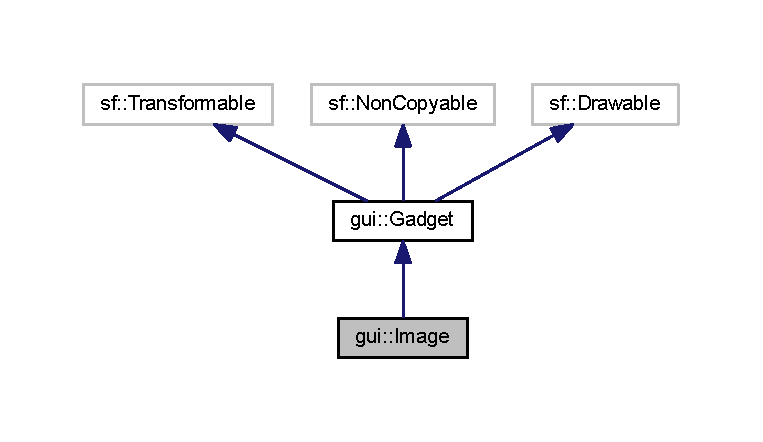
\includegraphics[width=350pt]{classgui_1_1_image__inherit__graph}
\end{center}
\end{figure}


Graphe de collaboration de gui\+:\+:Image\+:\nopagebreak
\begin{figure}[H]
\begin{center}
\leavevmode
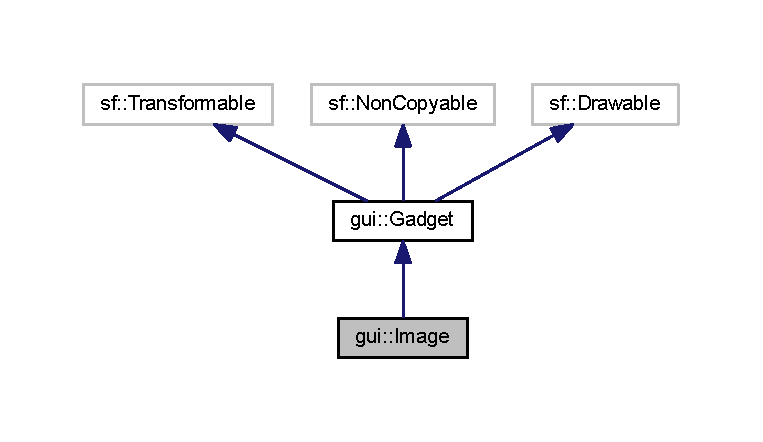
\includegraphics[width=350pt]{classgui_1_1_image__coll__graph}
\end{center}
\end{figure}
\subsection*{Fonctions membres publiques}
\begin{DoxyCompactItemize}
\item 
void \hyperlink{classgui_1_1_image_added38eba0bcb368cc15b6cfe2305a63}{traiter\+Evenements} (sf\+::\+Event evenement)
\begin{DoxyCompactList}\small\item\em Traitement des �venements clavier ou souris. \end{DoxyCompactList}\item 
void \hyperlink{classgui_1_1_image_a7ce4483de60aff2ec10c88156d890050}{actualiser} ()
\begin{DoxyCompactList}\small\item\em Actualiser les �l�ments de l\textquotesingle{}interface. \end{DoxyCompactList}\item 
virtual void \hyperlink{classgui_1_1_image_a6a2948c46b65fcf97646341936ec1aba}{draw} (sf\+::\+Render\+Target \&target, sf\+::\+Render\+States states) const 
\begin{DoxyCompactList}\small\item\em Dessine tout les �l�ments de l\textquotesingle{}interface. \end{DoxyCompactList}\end{DoxyCompactItemize}


\subsection{Description détaillée}
Une simple image. 

\subsection{Documentation des fonctions membres}
\index{gui\+::\+Image@{gui\+::\+Image}!actualiser@{actualiser}}
\index{actualiser@{actualiser}!gui\+::\+Image@{gui\+::\+Image}}
\subsubsection[{\texorpdfstring{actualiser()}{actualiser()}}]{\setlength{\rightskip}{0pt plus 5cm}void gui\+::\+Image\+::actualiser (
\begin{DoxyParamCaption}
{}
\end{DoxyParamCaption}
)}\hypertarget{classgui_1_1_image_a7ce4483de60aff2ec10c88156d890050}{}\label{classgui_1_1_image_a7ce4483de60aff2ec10c88156d890050}


Actualiser les �l�ments de l\textquotesingle{}interface. 

\index{gui\+::\+Image@{gui\+::\+Image}!draw@{draw}}
\index{draw@{draw}!gui\+::\+Image@{gui\+::\+Image}}
\subsubsection[{\texorpdfstring{draw(sf\+::\+Render\+Target \&target, sf\+::\+Render\+States states) const }{draw(sf::RenderTarget &target, sf::RenderStates states) const }}]{\setlength{\rightskip}{0pt plus 5cm}virtual void gui\+::\+Image\+::draw (
\begin{DoxyParamCaption}
\item[{sf\+::\+Render\+Target \&}]{target, }
\item[{sf\+::\+Render\+States}]{states}
\end{DoxyParamCaption}
) const\hspace{0.3cm}{\ttfamily [virtual]}}\hypertarget{classgui_1_1_image_a6a2948c46b65fcf97646341936ec1aba}{}\label{classgui_1_1_image_a6a2948c46b65fcf97646341936ec1aba}


Dessine tout les �l�ments de l\textquotesingle{}interface. 


\begin{DoxyParams}{Paramètres}
{\em target} & \\
\hline
{\em states} & \\
\hline
\end{DoxyParams}


Réimplémentée à partir de \hyperlink{classgui_1_1_gadget_a57b0c75601c7f6e0d43370013ae8c111}{gui\+::\+Gadget}.

\index{gui\+::\+Image@{gui\+::\+Image}!traiter\+Evenements@{traiter\+Evenements}}
\index{traiter\+Evenements@{traiter\+Evenements}!gui\+::\+Image@{gui\+::\+Image}}
\subsubsection[{\texorpdfstring{traiter\+Evenements(sf\+::\+Event evenement)}{traiterEvenements(sf::Event evenement)}}]{\setlength{\rightskip}{0pt plus 5cm}void gui\+::\+Image\+::traiter\+Evenements (
\begin{DoxyParamCaption}
\item[{sf\+::\+Event}]{evenement}
\end{DoxyParamCaption}
)}\hypertarget{classgui_1_1_image_added38eba0bcb368cc15b6cfe2305a63}{}\label{classgui_1_1_image_added38eba0bcb368cc15b6cfe2305a63}


Traitement des �venements clavier ou souris. 


\begin{DoxyParams}{Paramètres}
{\em evenement} & L\textquotesingle{}�venemnt � tratier. \\
\hline
\end{DoxyParams}


La documentation de cette classe a été générée à partir du fichier suivant \+:\begin{DoxyCompactItemize}
\item 
C\+:/\+Users/kris/\+One\+Drive/recherche Biome/01 -\/ code/code/include/gui/\hyperlink{_image_8h}{Image.\+h}\end{DoxyCompactItemize}

\hypertarget{classgui_1_1_interface_pheromones}{}\section{Référence de la classe gui\+:\+:Interface\+Pheromones}
\label{classgui_1_1_interface_pheromones}\index{gui\+::\+Interface\+Pheromones@{gui\+::\+Interface\+Pheromones}}


L\textquotesingle{}interface des ph�romones.  




{\ttfamily \#include $<$Interface\+Pheromones.\+h$>$}



Graphe d\textquotesingle{}héritage de gui\+:\+:Interface\+Pheromones\+:\nopagebreak
\begin{figure}[H]
\begin{center}
\leavevmode
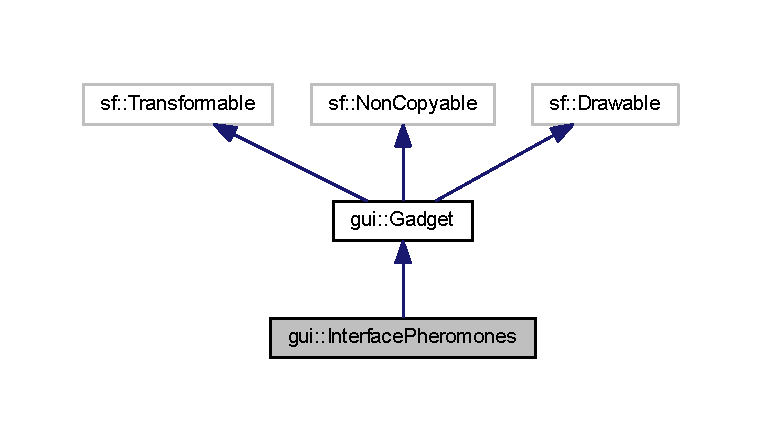
\includegraphics[width=350pt]{classgui_1_1_interface_pheromones__inherit__graph}
\end{center}
\end{figure}


Graphe de collaboration de gui\+:\+:Interface\+Pheromones\+:\nopagebreak
\begin{figure}[H]
\begin{center}
\leavevmode
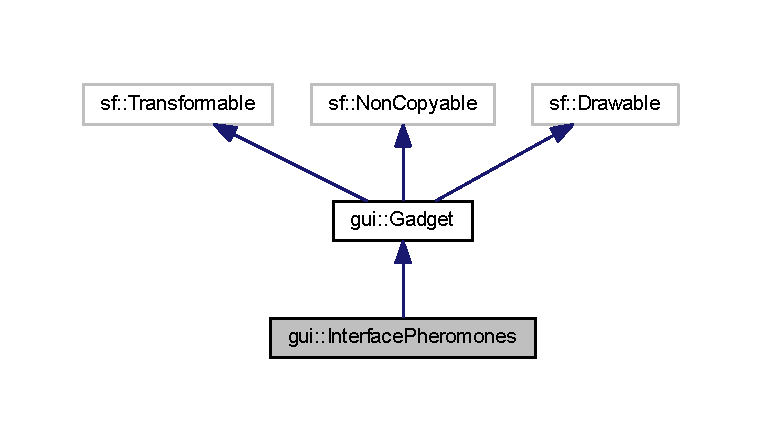
\includegraphics[width=350pt]{classgui_1_1_interface_pheromones__coll__graph}
\end{center}
\end{figure}
\subsection*{Fonctions membres publiques}
\begin{DoxyCompactItemize}
\item 
void \hyperlink{classgui_1_1_interface_pheromones_a3b0b5b85d96a0d5c4436c511e3a18760}{traiter\+Evenements} (sf\+::\+Event evenement)
\begin{DoxyCompactList}\small\item\em Traitement des �venements clavier ou souris. \end{DoxyCompactList}\item 
void \hyperlink{classgui_1_1_interface_pheromones_a2f255574548639c0360278d3c0b2e20b}{actualiser} ()
\begin{DoxyCompactList}\small\item\em Actualiser les �l�ments de l\textquotesingle{}interface. \end{DoxyCompactList}\item 
virtual void \hyperlink{classgui_1_1_interface_pheromones_a970a5c6ef20546ecf0905660c5d0c62a}{draw} (sf\+::\+Render\+Target \&target, sf\+::\+Render\+States states) const 
\begin{DoxyCompactList}\small\item\em Dessine tout les �l�ments de l\textquotesingle{}interface. \end{DoxyCompactList}\end{DoxyCompactItemize}


\subsection{Description détaillée}
L\textquotesingle{}interface des ph�romones. 

\subsection{Documentation des fonctions membres}
\index{gui\+::\+Interface\+Pheromones@{gui\+::\+Interface\+Pheromones}!actualiser@{actualiser}}
\index{actualiser@{actualiser}!gui\+::\+Interface\+Pheromones@{gui\+::\+Interface\+Pheromones}}
\subsubsection[{\texorpdfstring{actualiser()}{actualiser()}}]{\setlength{\rightskip}{0pt plus 5cm}void gui\+::\+Interface\+Pheromones\+::actualiser (
\begin{DoxyParamCaption}
{}
\end{DoxyParamCaption}
)}\hypertarget{classgui_1_1_interface_pheromones_a2f255574548639c0360278d3c0b2e20b}{}\label{classgui_1_1_interface_pheromones_a2f255574548639c0360278d3c0b2e20b}


Actualiser les �l�ments de l\textquotesingle{}interface. 

\index{gui\+::\+Interface\+Pheromones@{gui\+::\+Interface\+Pheromones}!draw@{draw}}
\index{draw@{draw}!gui\+::\+Interface\+Pheromones@{gui\+::\+Interface\+Pheromones}}
\subsubsection[{\texorpdfstring{draw(sf\+::\+Render\+Target \&target, sf\+::\+Render\+States states) const }{draw(sf::RenderTarget &target, sf::RenderStates states) const }}]{\setlength{\rightskip}{0pt plus 5cm}virtual void gui\+::\+Interface\+Pheromones\+::draw (
\begin{DoxyParamCaption}
\item[{sf\+::\+Render\+Target \&}]{target, }
\item[{sf\+::\+Render\+States}]{states}
\end{DoxyParamCaption}
) const\hspace{0.3cm}{\ttfamily [virtual]}}\hypertarget{classgui_1_1_interface_pheromones_a970a5c6ef20546ecf0905660c5d0c62a}{}\label{classgui_1_1_interface_pheromones_a970a5c6ef20546ecf0905660c5d0c62a}


Dessine tout les �l�ments de l\textquotesingle{}interface. 


\begin{DoxyParams}{Paramètres}
{\em target} & \\
\hline
{\em states} & \\
\hline
\end{DoxyParams}


Réimplémentée à partir de \hyperlink{classgui_1_1_gadget_a57b0c75601c7f6e0d43370013ae8c111}{gui\+::\+Gadget}.

\index{gui\+::\+Interface\+Pheromones@{gui\+::\+Interface\+Pheromones}!traiter\+Evenements@{traiter\+Evenements}}
\index{traiter\+Evenements@{traiter\+Evenements}!gui\+::\+Interface\+Pheromones@{gui\+::\+Interface\+Pheromones}}
\subsubsection[{\texorpdfstring{traiter\+Evenements(sf\+::\+Event evenement)}{traiterEvenements(sf::Event evenement)}}]{\setlength{\rightskip}{0pt plus 5cm}void gui\+::\+Interface\+Pheromones\+::traiter\+Evenements (
\begin{DoxyParamCaption}
\item[{sf\+::\+Event}]{evenement}
\end{DoxyParamCaption}
)}\hypertarget{classgui_1_1_interface_pheromones_a3b0b5b85d96a0d5c4436c511e3a18760}{}\label{classgui_1_1_interface_pheromones_a3b0b5b85d96a0d5c4436c511e3a18760}


Traitement des �venements clavier ou souris. 


\begin{DoxyParams}{Paramètres}
{\em evenement} & L\textquotesingle{}�venemnt � tratier. \\
\hline
\end{DoxyParams}


La documentation de cette classe a été générée à partir du fichier suivant \+:\begin{DoxyCompactItemize}
\item 
C\+:/\+Users/kris/\+One\+Drive/recherche Biome/01 -\/ code/code/include/gui/\hyperlink{_interface_pheromones_8h}{Interface\+Pheromones.\+h}\end{DoxyCompactItemize}

\hypertarget{classjeu_1_1_jeu}{}\section{Référence de la classe jeu\+:\+:Jeu}
\label{classjeu_1_1_jeu}\index{jeu\+::\+Jeu@{jeu\+::\+Jeu}}


La classe g�n�ral du jeu, g�re le jeu de mani�re global. popo autre ligne l� aussi.  




{\ttfamily \#include $<$Jeu.\+h$>$}



Graphe d\textquotesingle{}héritage de jeu\+:\+:Jeu\+:\nopagebreak
\begin{figure}[H]
\begin{center}
\leavevmode
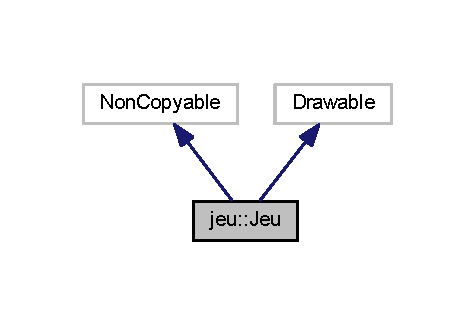
\includegraphics[width=228pt]{classjeu_1_1_jeu__inherit__graph}
\end{center}
\end{figure}


Graphe de collaboration de jeu\+:\+:Jeu\+:\nopagebreak
\begin{figure}[H]
\begin{center}
\leavevmode
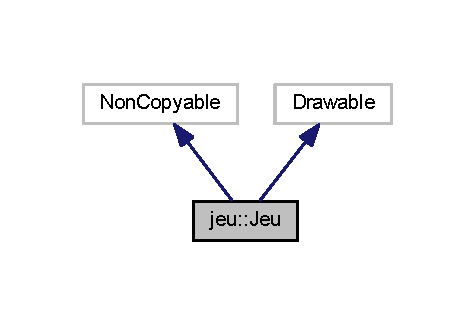
\includegraphics[width=228pt]{classjeu_1_1_jeu__coll__graph}
\end{center}
\end{figure}
\subsection*{Fonctions membres publiques}
\begin{DoxyCompactItemize}
\item 
void \hyperlink{classjeu_1_1_jeu_ab2a947b1bcf23bfc03055e44ef3f1b97}{demarrer\+Partie} ()
\begin{DoxyCompactList}\small\item\em D�marre une nouvelle partie. et l� onsaute une ligne. et une autre. \end{DoxyCompactList}\item 
void \hyperlink{classjeu_1_1_jeu_a3db176776c68ecf18e4b295496d962b4}{quitter\+Partie} ()
\begin{DoxyCompactList}\small\item\em Quitter la partie en cours (sans sauvegarde). \end{DoxyCompactList}\item 
void \hyperlink{classjeu_1_1_jeu_a8a4797dd1509a9f81da923f6bdff7796}{charger\+Partie} ()
\begin{DoxyCompactList}\small\item\em Charger une partie precedement sauvegarder. \end{DoxyCompactList}\item 
void \hyperlink{classjeu_1_1_jeu_a61a3a44e5de01e55376caf7b31785931}{sauvegarder\+Partie} ()
\begin{DoxyCompactList}\small\item\em Sauvegarder une partie. \end{DoxyCompactList}\item 
void \hyperlink{classjeu_1_1_jeu_ad387370139d955b86a92d1cd4d9becd8}{actualiser} (sf\+::\+Time deltaT=sf\+::\+Time\+::\+Zero)
\begin{DoxyCompactList}\small\item\em Actualiser les �l�ments du jeu. \end{DoxyCompactList}\item 
void \hyperlink{classjeu_1_1_jeu_acf25c03f9a224e223aec9e2540ca8aa0}{traiter\+Evenements} (sf\+::\+Event evenement)
\begin{DoxyCompactList}\small\item\em Traitement des �venemnts clavier et souris. \end{DoxyCompactList}\item 
virtual void \hyperlink{classjeu_1_1_jeu_a9c6b7bee6497df47fab172f87048c725}{draw} (sf\+::\+Render\+Target \&target, sf\+::\+Render\+States states) const 
\end{DoxyCompactItemize}


\subsection{Description détaillée}
La classe g�n�ral du jeu, g�re le jeu de mani�re global. popo autre ligne l� aussi. 

\subsection{Documentation des fonctions membres}
\index{jeu\+::\+Jeu@{jeu\+::\+Jeu}!actualiser@{actualiser}}
\index{actualiser@{actualiser}!jeu\+::\+Jeu@{jeu\+::\+Jeu}}
\subsubsection[{\texorpdfstring{actualiser(sf\+::\+Time delta\+T=sf\+::\+Time\+::\+Zero)}{actualiser(sf::Time deltaT=sf::Time::Zero)}}]{\setlength{\rightskip}{0pt plus 5cm}void jeu\+::\+Jeu\+::actualiser (
\begin{DoxyParamCaption}
\item[{sf\+::\+Time}]{deltaT = {\ttfamily sf\+:\+:Time\+:\+:Zero}}
\end{DoxyParamCaption}
)}\hypertarget{classjeu_1_1_jeu_ad387370139d955b86a92d1cd4d9becd8}{}\label{classjeu_1_1_jeu_ad387370139d955b86a92d1cd4d9becd8}


Actualiser les �l�ments du jeu. 


\begin{DoxyParams}{Paramètres}
{\em deltaT} & Temps �coul� depuis la derni�re actualisation. ( par d�faut = 0\+: Actualise sans tenir compte du temps ecoul�) \\
\hline
\end{DoxyParams}
\index{jeu\+::\+Jeu@{jeu\+::\+Jeu}!charger\+Partie@{charger\+Partie}}
\index{charger\+Partie@{charger\+Partie}!jeu\+::\+Jeu@{jeu\+::\+Jeu}}
\subsubsection[{\texorpdfstring{charger\+Partie()}{chargerPartie()}}]{\setlength{\rightskip}{0pt plus 5cm}void jeu\+::\+Jeu\+::charger\+Partie (
\begin{DoxyParamCaption}
{}
\end{DoxyParamCaption}
)}\hypertarget{classjeu_1_1_jeu_a8a4797dd1509a9f81da923f6bdff7796}{}\label{classjeu_1_1_jeu_a8a4797dd1509a9f81da923f6bdff7796}


Charger une partie precedement sauvegarder. 

\index{jeu\+::\+Jeu@{jeu\+::\+Jeu}!demarrer\+Partie@{demarrer\+Partie}}
\index{demarrer\+Partie@{demarrer\+Partie}!jeu\+::\+Jeu@{jeu\+::\+Jeu}}
\subsubsection[{\texorpdfstring{demarrer\+Partie()}{demarrerPartie()}}]{\setlength{\rightskip}{0pt plus 5cm}void jeu\+::\+Jeu\+::demarrer\+Partie (
\begin{DoxyParamCaption}
{}
\end{DoxyParamCaption}
)}\hypertarget{classjeu_1_1_jeu_ab2a947b1bcf23bfc03055e44ef3f1b97}{}\label{classjeu_1_1_jeu_ab2a947b1bcf23bfc03055e44ef3f1b97}


D�marre une nouvelle partie. et l� onsaute une ligne. et une autre. 

\index{jeu\+::\+Jeu@{jeu\+::\+Jeu}!draw@{draw}}
\index{draw@{draw}!jeu\+::\+Jeu@{jeu\+::\+Jeu}}
\subsubsection[{\texorpdfstring{draw(sf\+::\+Render\+Target \&target, sf\+::\+Render\+States states) const }{draw(sf::RenderTarget &target, sf::RenderStates states) const }}]{\setlength{\rightskip}{0pt plus 5cm}virtual void jeu\+::\+Jeu\+::draw (
\begin{DoxyParamCaption}
\item[{sf\+::\+Render\+Target \&}]{target, }
\item[{sf\+::\+Render\+States}]{states}
\end{DoxyParamCaption}
) const\hspace{0.3cm}{\ttfamily [virtual]}}\hypertarget{classjeu_1_1_jeu_a9c6b7bee6497df47fab172f87048c725}{}\label{classjeu_1_1_jeu_a9c6b7bee6497df47fab172f87048c725}
\index{jeu\+::\+Jeu@{jeu\+::\+Jeu}!quitter\+Partie@{quitter\+Partie}}
\index{quitter\+Partie@{quitter\+Partie}!jeu\+::\+Jeu@{jeu\+::\+Jeu}}
\subsubsection[{\texorpdfstring{quitter\+Partie()}{quitterPartie()}}]{\setlength{\rightskip}{0pt plus 5cm}void jeu\+::\+Jeu\+::quitter\+Partie (
\begin{DoxyParamCaption}
{}
\end{DoxyParamCaption}
)}\hypertarget{classjeu_1_1_jeu_a3db176776c68ecf18e4b295496d962b4}{}\label{classjeu_1_1_jeu_a3db176776c68ecf18e4b295496d962b4}


Quitter la partie en cours (sans sauvegarde). 

\index{jeu\+::\+Jeu@{jeu\+::\+Jeu}!sauvegarder\+Partie@{sauvegarder\+Partie}}
\index{sauvegarder\+Partie@{sauvegarder\+Partie}!jeu\+::\+Jeu@{jeu\+::\+Jeu}}
\subsubsection[{\texorpdfstring{sauvegarder\+Partie()}{sauvegarderPartie()}}]{\setlength{\rightskip}{0pt plus 5cm}void jeu\+::\+Jeu\+::sauvegarder\+Partie (
\begin{DoxyParamCaption}
{}
\end{DoxyParamCaption}
)}\hypertarget{classjeu_1_1_jeu_a61a3a44e5de01e55376caf7b31785931}{}\label{classjeu_1_1_jeu_a61a3a44e5de01e55376caf7b31785931}


Sauvegarder une partie. 

\index{jeu\+::\+Jeu@{jeu\+::\+Jeu}!traiter\+Evenements@{traiter\+Evenements}}
\index{traiter\+Evenements@{traiter\+Evenements}!jeu\+::\+Jeu@{jeu\+::\+Jeu}}
\subsubsection[{\texorpdfstring{traiter\+Evenements(sf\+::\+Event evenement)}{traiterEvenements(sf::Event evenement)}}]{\setlength{\rightskip}{0pt plus 5cm}void jeu\+::\+Jeu\+::traiter\+Evenements (
\begin{DoxyParamCaption}
\item[{sf\+::\+Event}]{evenement}
\end{DoxyParamCaption}
)}\hypertarget{classjeu_1_1_jeu_acf25c03f9a224e223aec9e2540ca8aa0}{}\label{classjeu_1_1_jeu_acf25c03f9a224e223aec9e2540ca8aa0}


Traitement des �venemnts clavier et souris. 


\begin{DoxyParams}{Paramètres}
{\em evenement} & l\textquotesingle{}�venement � traiter. \\
\hline
\end{DoxyParams}


La documentation de cette classe a été générée à partir du fichier suivant \+:\begin{DoxyCompactItemize}
\item 
C\+:/\+Users/kris/\+One\+Drive/recherche Biome/01 -\/ code/code/include/jeu/\hyperlink{_jeu_8h}{Jeu.\+h}\end{DoxyCompactItemize}

\hypertarget{classgui_1_1_label}{}\section{Référence de la classe gui\+:\+:Label}
\label{classgui_1_1_label}\index{gui\+::\+Label@{gui\+::\+Label}}


Un simple label.  




{\ttfamily \#include $<$Label.\+h$>$}



Graphe d\textquotesingle{}héritage de gui\+:\+:Label\+:\nopagebreak
\begin{figure}[H]
\begin{center}
\leavevmode
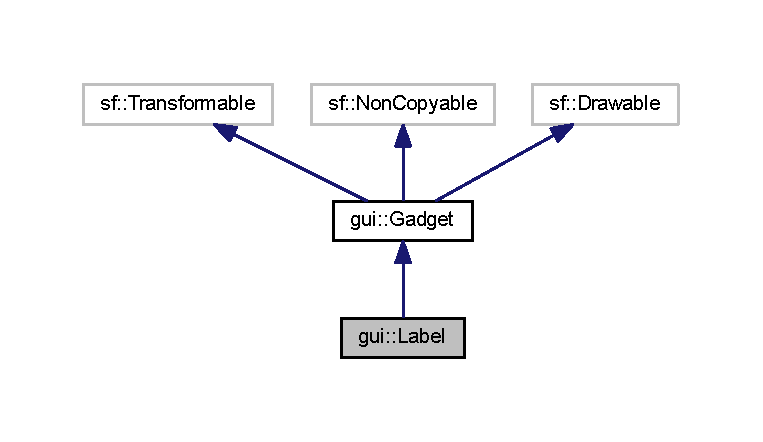
\includegraphics[width=350pt]{classgui_1_1_label__inherit__graph}
\end{center}
\end{figure}


Graphe de collaboration de gui\+:\+:Label\+:\nopagebreak
\begin{figure}[H]
\begin{center}
\leavevmode
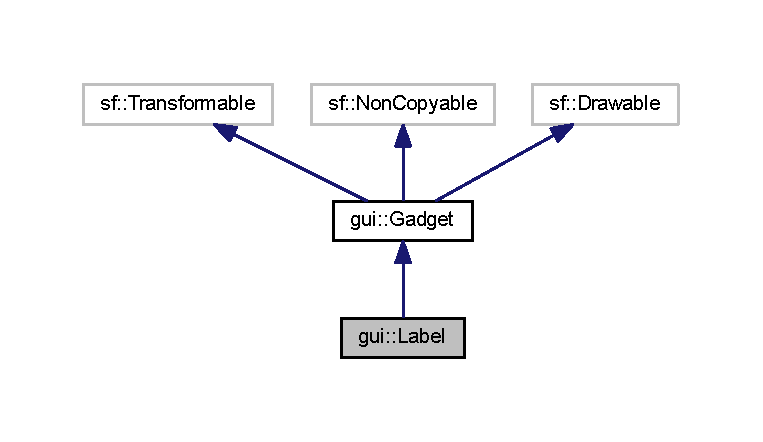
\includegraphics[width=350pt]{classgui_1_1_label__coll__graph}
\end{center}
\end{figure}
\subsection*{Fonctions membres publiques}
\begin{DoxyCompactItemize}
\item 
void \hyperlink{classgui_1_1_label_ab19d265bc861ffa5dbe88984a85d0636}{traiter\+Evenements} (sf\+::\+Event evenement)
\begin{DoxyCompactList}\small\item\em Traitement des �venements clavier ou souris. \end{DoxyCompactList}\item 
void \hyperlink{classgui_1_1_label_af807726e00c95695a8ed8ee60a898b6a}{actualiser} ()
\begin{DoxyCompactList}\small\item\em Actualiser les �l�ments de l\textquotesingle{}interface. \end{DoxyCompactList}\item 
virtual void \hyperlink{classgui_1_1_label_a835406d1bc730f86ab715fc70c4541ca}{draw} (sf\+::\+Render\+Target \&target, sf\+::\+Render\+States states) const 
\begin{DoxyCompactList}\small\item\em Dessine tout les �l�ments de l\textquotesingle{}interface. \end{DoxyCompactList}\end{DoxyCompactItemize}


\subsection{Description détaillée}
Un simple label. 

\subsection{Documentation des fonctions membres}
\index{gui\+::\+Label@{gui\+::\+Label}!actualiser@{actualiser}}
\index{actualiser@{actualiser}!gui\+::\+Label@{gui\+::\+Label}}
\subsubsection[{\texorpdfstring{actualiser()}{actualiser()}}]{\setlength{\rightskip}{0pt plus 5cm}void gui\+::\+Label\+::actualiser (
\begin{DoxyParamCaption}
{}
\end{DoxyParamCaption}
)}\hypertarget{classgui_1_1_label_af807726e00c95695a8ed8ee60a898b6a}{}\label{classgui_1_1_label_af807726e00c95695a8ed8ee60a898b6a}


Actualiser les �l�ments de l\textquotesingle{}interface. 

\index{gui\+::\+Label@{gui\+::\+Label}!draw@{draw}}
\index{draw@{draw}!gui\+::\+Label@{gui\+::\+Label}}
\subsubsection[{\texorpdfstring{draw(sf\+::\+Render\+Target \&target, sf\+::\+Render\+States states) const }{draw(sf::RenderTarget &target, sf::RenderStates states) const }}]{\setlength{\rightskip}{0pt plus 5cm}virtual void gui\+::\+Label\+::draw (
\begin{DoxyParamCaption}
\item[{sf\+::\+Render\+Target \&}]{target, }
\item[{sf\+::\+Render\+States}]{states}
\end{DoxyParamCaption}
) const\hspace{0.3cm}{\ttfamily [virtual]}}\hypertarget{classgui_1_1_label_a835406d1bc730f86ab715fc70c4541ca}{}\label{classgui_1_1_label_a835406d1bc730f86ab715fc70c4541ca}


Dessine tout les �l�ments de l\textquotesingle{}interface. 


\begin{DoxyParams}{Paramètres}
{\em target} & \\
\hline
{\em states} & \\
\hline
\end{DoxyParams}


Réimplémentée à partir de \hyperlink{classgui_1_1_gadget_a57b0c75601c7f6e0d43370013ae8c111}{gui\+::\+Gadget}.

\index{gui\+::\+Label@{gui\+::\+Label}!traiter\+Evenements@{traiter\+Evenements}}
\index{traiter\+Evenements@{traiter\+Evenements}!gui\+::\+Label@{gui\+::\+Label}}
\subsubsection[{\texorpdfstring{traiter\+Evenements(sf\+::\+Event evenement)}{traiterEvenements(sf::Event evenement)}}]{\setlength{\rightskip}{0pt plus 5cm}void gui\+::\+Label\+::traiter\+Evenements (
\begin{DoxyParamCaption}
\item[{sf\+::\+Event}]{evenement}
\end{DoxyParamCaption}
)}\hypertarget{classgui_1_1_label_ab19d265bc861ffa5dbe88984a85d0636}{}\label{classgui_1_1_label_ab19d265bc861ffa5dbe88984a85d0636}


Traitement des �venements clavier ou souris. 


\begin{DoxyParams}{Paramètres}
{\em evenement} & L\textquotesingle{}�venemnt � tratier. \\
\hline
\end{DoxyParams}


La documentation de cette classe a été générée à partir du fichier suivant \+:\begin{DoxyCompactItemize}
\item 
C\+:/\+Users/kris/\+One\+Drive/recherche Biome/01 -\/ code/code/include/gui/\hyperlink{_label_8h}{Label.\+h}\end{DoxyCompactItemize}

\hypertarget{classjeu_1_1_plante_verte}{}\section{Référence de la classe jeu\+:\+:Plante\+Verte}
\label{classjeu_1_1_plante_verte}\index{jeu\+::\+Plante\+Verte@{jeu\+::\+Plante\+Verte}}


Une plante verte apporte de la nourriture aux fourmis et autres insectes du biome.  




{\ttfamily \#include $<$Plante\+Verte.\+h$>$}



Graphe d\textquotesingle{}héritage de jeu\+:\+:Plante\+Verte\+:\nopagebreak
\begin{figure}[H]
\begin{center}
\leavevmode
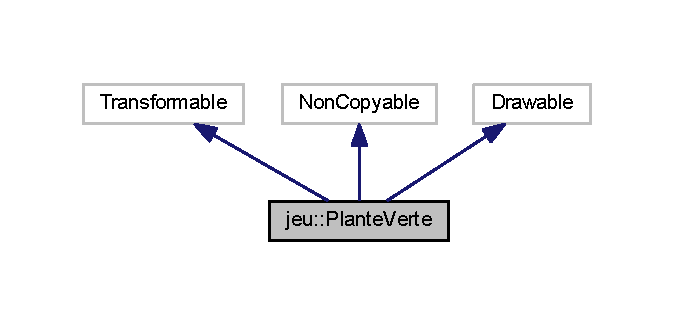
\includegraphics[width=324pt]{classjeu_1_1_plante_verte__inherit__graph}
\end{center}
\end{figure}


Graphe de collaboration de jeu\+:\+:Plante\+Verte\+:\nopagebreak
\begin{figure}[H]
\begin{center}
\leavevmode
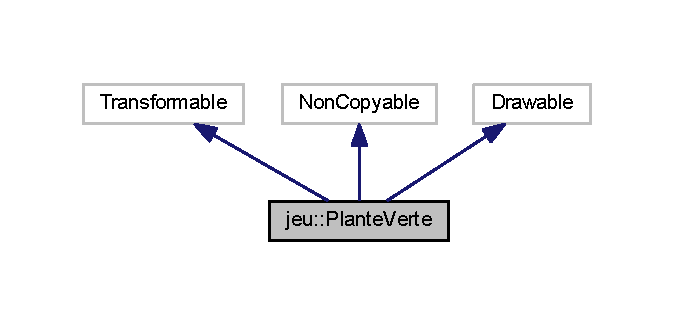
\includegraphics[width=324pt]{classjeu_1_1_plante_verte__coll__graph}
\end{center}
\end{figure}


\subsection{Description détaillée}
Une plante verte apporte de la nourriture aux fourmis et autres insectes du biome. 

La documentation de cette classe a été générée à partir du fichier suivant \+:\begin{DoxyCompactItemize}
\item 
C\+:/\+Users/kris/\+One\+Drive/recherche Biome/01 -\/ code/code/include/jeu/\hyperlink{_plante_verte_8h}{Plante\+Verte.\+h}\end{DoxyCompactItemize}

\hypertarget{classapp_1_1_resource_mgr}{}\section{Référence du modèle de la classe app\+:\+:Resource\+Mgr$<$ R\+E\+S\+O\+U\+R\+CE, I\+D\+E\+N\+T\+I\+F\+I\+A\+NT $>$}
\label{classapp_1_1_resource_mgr}\index{app\+::\+Resource\+Mgr$<$ R\+E\+S\+O\+U\+R\+C\+E, I\+D\+E\+N\+T\+I\+F\+I\+A\+N\+T $>$@{app\+::\+Resource\+Mgr$<$ R\+E\+S\+O\+U\+R\+C\+E, I\+D\+E\+N\+T\+I\+F\+I\+A\+N\+T $>$}}


Manager de ressource (polices, images).  




{\ttfamily \#include $<$Resource\+Mgr.\+h$>$}

\subsection*{Fonctions membres publiques}
\begin{DoxyCompactItemize}
\item 
\hyperlink{classapp_1_1_resource_mgr_a4f95e4f251a11a0cf368ed8b074fd297}{Resource\+Mgr} (const \hyperlink{classapp_1_1_resource_mgr}{Resource\+Mgr} \&)=delete
\begin{DoxyCompactList}\small\item\em constructeur par copie \end{DoxyCompactList}\item 
\hyperlink{classapp_1_1_resource_mgr_a9bb6d183effa248577c9e6df24f948ef}{Resource\+Mgr} ()=default
\begin{DoxyCompactList}\small\item\em Constructeur. \end{DoxyCompactList}\item 
\hyperlink{classapp_1_1_resource_mgr}{Resource\+Mgr} \& \hyperlink{classapp_1_1_resource_mgr_a8c06cc4165068e7aae8ba2aa505d4c1a}{operator=} (const \hyperlink{classapp_1_1_resource_mgr}{Resource\+Mgr} \&)=delete
\begin{DoxyCompactList}\small\item\em Surcharge de =. \end{DoxyCompactList}\item 
{\footnotesize template$<$typename... Args$>$ }\\void \hyperlink{classapp_1_1_resource_mgr_a43174877ac3bce3b43b68f94e0eb2815}{load} (const I\+D\+E\+N\+T\+I\+F\+I\+A\+NT \&id, Args \&\&...args)
\begin{DoxyCompactList}\small\item\em Charger une image ou une police depuis un fichier et l\textquotesingle{}associe � un identifiant. \end{DoxyCompactList}\item 
R\+E\+S\+O\+U\+R\+CE \& \hyperlink{classapp_1_1_resource_mgr_a6d50e13d521942530229e80f660ff004}{get} (const I\+D\+E\+N\+T\+I\+F\+I\+A\+NT \&id) const 
\begin{DoxyCompactList}\small\item\em demande une image ou une police � partir de son identifiant. \end{DoxyCompactList}\end{DoxyCompactItemize}


\subsection{Description détaillée}
\subsubsection*{template$<$typename R\+E\+S\+O\+U\+R\+CE, typename I\+D\+E\+N\+T\+I\+F\+I\+A\+NT = int$>$\\*
class app\+::\+Resource\+Mgr$<$ R\+E\+S\+O\+U\+R\+C\+E, I\+D\+E\+N\+T\+I\+F\+I\+A\+N\+T $>$}

Manager de ressource (polices, images). 

Classe template des polices, images

G�re les ressource fa�on R\+A\+II

\begin{DoxySeeAlso}{Voir également}
\hyperlink{classapp_1_1_ecran}{app\+::\+Ecran}, \hyperlink{classapp_1_1_gestion__ecrans}{app\+::\+Gestion\+\_\+ecrans} 
\end{DoxySeeAlso}


\subsection{Documentation des constructeurs et destructeur}
\index{app\+::\+Resource\+Mgr@{app\+::\+Resource\+Mgr}!Resource\+Mgr@{Resource\+Mgr}}
\index{Resource\+Mgr@{Resource\+Mgr}!app\+::\+Resource\+Mgr@{app\+::\+Resource\+Mgr}}
\subsubsection[{\texorpdfstring{Resource\+Mgr(const Resource\+Mgr \&)=delete}{ResourceMgr(const ResourceMgr &)=delete}}]{\setlength{\rightskip}{0pt plus 5cm}template$<$typename R\+E\+S\+O\+U\+R\+CE , typename I\+D\+E\+N\+T\+I\+F\+I\+A\+NT  = int$>$ {\bf app\+::\+Resource\+Mgr}$<$ R\+E\+S\+O\+U\+R\+CE, I\+D\+E\+N\+T\+I\+F\+I\+A\+NT $>$\+::{\bf Resource\+Mgr} (
\begin{DoxyParamCaption}
\item[{const {\bf Resource\+Mgr}$<$ R\+E\+S\+O\+U\+R\+CE, I\+D\+E\+N\+T\+I\+F\+I\+A\+NT $>$ \&}]{}
\end{DoxyParamCaption}
)\hspace{0.3cm}{\ttfamily [delete]}}\hypertarget{classapp_1_1_resource_mgr_a4f95e4f251a11a0cf368ed8b074fd297}{}\label{classapp_1_1_resource_mgr_a4f95e4f251a11a0cf368ed8b074fd297}


constructeur par copie 

\char`\"{}= delete\char`\"{} c\textquotesingle{}est une mani�re de dire non copyable si j\textquotesingle{}ai bien compris, cf le bouquin S\+F\+ML ... \index{app\+::\+Resource\+Mgr@{app\+::\+Resource\+Mgr}!Resource\+Mgr@{Resource\+Mgr}}
\index{Resource\+Mgr@{Resource\+Mgr}!app\+::\+Resource\+Mgr@{app\+::\+Resource\+Mgr}}
\subsubsection[{\texorpdfstring{Resource\+Mgr()=default}{ResourceMgr()=default}}]{\setlength{\rightskip}{0pt plus 5cm}template$<$typename R\+E\+S\+O\+U\+R\+CE , typename I\+D\+E\+N\+T\+I\+F\+I\+A\+NT  = int$>$ {\bf app\+::\+Resource\+Mgr}$<$ R\+E\+S\+O\+U\+R\+CE, I\+D\+E\+N\+T\+I\+F\+I\+A\+NT $>$\+::{\bf Resource\+Mgr} (
\begin{DoxyParamCaption}
{}
\end{DoxyParamCaption}
)\hspace{0.3cm}{\ttfamily [default]}}\hypertarget{classapp_1_1_resource_mgr_a9bb6d183effa248577c9e6df24f948ef}{}\label{classapp_1_1_resource_mgr_a9bb6d183effa248577c9e6df24f948ef}


Constructeur. 

\char`\"{}= default\char`\"{} cf le bouquin S\+F\+ML ... 

\subsection{Documentation des fonctions membres}
\index{app\+::\+Resource\+Mgr@{app\+::\+Resource\+Mgr}!get@{get}}
\index{get@{get}!app\+::\+Resource\+Mgr@{app\+::\+Resource\+Mgr}}
\subsubsection[{\texorpdfstring{get(const I\+D\+E\+N\+T\+I\+F\+I\+A\+N\+T \&id) const }{get(const IDENTIFIANT &id) const }}]{\setlength{\rightskip}{0pt plus 5cm}template$<$typename R\+E\+S\+O\+U\+R\+CE , typename I\+D\+E\+N\+T\+I\+F\+I\+A\+NT $>$ R\+E\+S\+O\+U\+R\+CE \& {\bf app\+::\+Resource\+Mgr}$<$ R\+E\+S\+O\+U\+R\+CE, I\+D\+E\+N\+T\+I\+F\+I\+A\+NT $>$\+::get (
\begin{DoxyParamCaption}
\item[{const I\+D\+E\+N\+T\+I\+F\+I\+A\+NT \&}]{id}
\end{DoxyParamCaption}
) const}\hypertarget{classapp_1_1_resource_mgr_a6d50e13d521942530229e80f660ff004}{}\label{classapp_1_1_resource_mgr_a6d50e13d521942530229e80f660ff004}


demande une image ou une police � partir de son identifiant. 


\begin{DoxyParams}{Paramètres}
{\em id} & l\textquotesingle{}identenfiant \\
\hline
\end{DoxyParams}
\begin{DoxyReturn}{Renvoie}
la ressource demand�. 
\end{DoxyReturn}
\index{app\+::\+Resource\+Mgr@{app\+::\+Resource\+Mgr}!load@{load}}
\index{load@{load}!app\+::\+Resource\+Mgr@{app\+::\+Resource\+Mgr}}
\subsubsection[{\texorpdfstring{load(const I\+D\+E\+N\+T\+I\+F\+I\+A\+N\+T \&id, Args \&\&...\+args)}{load(const IDENTIFIANT &id, Args &&...args)}}]{\setlength{\rightskip}{0pt plus 5cm}template$<$typename R\+E\+S\+O\+U\+R\+CE , typename I\+D\+E\+N\+T\+I\+F\+I\+A\+NT $>$ template$<$typename... Args$>$ void {\bf app\+::\+Resource\+Mgr}$<$ R\+E\+S\+O\+U\+R\+CE, I\+D\+E\+N\+T\+I\+F\+I\+A\+NT $>$\+::load (
\begin{DoxyParamCaption}
\item[{const I\+D\+E\+N\+T\+I\+F\+I\+A\+NT \&}]{id, }
\item[{Args \&\&...}]{args}
\end{DoxyParamCaption}
)}\hypertarget{classapp_1_1_resource_mgr_a43174877ac3bce3b43b68f94e0eb2815}{}\label{classapp_1_1_resource_mgr_a43174877ac3bce3b43b68f94e0eb2815}


Charger une image ou une police depuis un fichier et l\textquotesingle{}associe � un identifiant. 

Manager de ressource.


\begin{DoxyParams}{Paramètres}
{\em id} & l\textquotesingle{}identenfiant \\
\hline
{\em args} & le fichier\\
\hline
\end{DoxyParams}
Class template des polices, images \index{app\+::\+Resource\+Mgr@{app\+::\+Resource\+Mgr}!operator=@{operator=}}
\index{operator=@{operator=}!app\+::\+Resource\+Mgr@{app\+::\+Resource\+Mgr}}
\subsubsection[{\texorpdfstring{operator=(const Resource\+Mgr \&)=delete}{operator=(const ResourceMgr &)=delete}}]{\setlength{\rightskip}{0pt plus 5cm}template$<$typename R\+E\+S\+O\+U\+R\+CE , typename I\+D\+E\+N\+T\+I\+F\+I\+A\+NT  = int$>$ {\bf Resource\+Mgr}\& {\bf app\+::\+Resource\+Mgr}$<$ R\+E\+S\+O\+U\+R\+CE, I\+D\+E\+N\+T\+I\+F\+I\+A\+NT $>$\+::operator= (
\begin{DoxyParamCaption}
\item[{const {\bf Resource\+Mgr}$<$ R\+E\+S\+O\+U\+R\+CE, I\+D\+E\+N\+T\+I\+F\+I\+A\+NT $>$ \&}]{}
\end{DoxyParamCaption}
)\hspace{0.3cm}{\ttfamily [delete]}}\hypertarget{classapp_1_1_resource_mgr_a8c06cc4165068e7aae8ba2aa505d4c1a}{}\label{classapp_1_1_resource_mgr_a8c06cc4165068e7aae8ba2aa505d4c1a}


Surcharge de =. 

\char`\"{}= delete\char`\"{} cf le bouquin S\+F\+ML, mais je crois que c\textquotesingle{}est pour dire ope= c\textquotesingle{}est copy...bref pas super claire encore 

La documentation de cette classe a été générée à partir des fichiers suivants \+:\begin{DoxyCompactItemize}
\item 
C\+:/\+Users/kris/\+One\+Drive/recherche Biome/01 -\/ code/code/include/appli/\hyperlink{_resource_mgr_8h}{Resource\+Mgr.\+h}\item 
C\+:/\+Users/kris/\+One\+Drive/recherche Biome/01 -\/ code/code/include/appli/\hyperlink{_resource_mgr_8inl}{Resource\+Mgr.\+inl}\end{DoxyCompactItemize}

\hypertarget{classapp_1_1_resource_mgr_3_01sf_1_1_music_00_01_i_d_e_n_t_i_f_i_a_n_t_01_4}{}\section{Référence du modèle de la classe app\+:\+:Resource\+Mgr$<$ sf\+:\+:Music, I\+D\+E\+N\+T\+I\+F\+I\+A\+NT $>$}
\label{classapp_1_1_resource_mgr_3_01sf_1_1_music_00_01_i_d_e_n_t_i_f_i_a_n_t_01_4}\index{app\+::\+Resource\+Mgr$<$ sf\+::\+Music, I\+D\+E\+N\+T\+I\+F\+I\+A\+N\+T $>$@{app\+::\+Resource\+Mgr$<$ sf\+::\+Music, I\+D\+E\+N\+T\+I\+F\+I\+A\+N\+T $>$}}


Manager de ressource (music).  




{\ttfamily \#include $<$Resource\+Mgr.\+h$>$}

\subsection*{Fonctions membres publiques}
\begin{DoxyCompactItemize}
\item 
\hyperlink{classapp_1_1_resource_mgr_3_01sf_1_1_music_00_01_i_d_e_n_t_i_f_i_a_n_t_01_4_a303e951921bbc6db156bf4bdb8cfddd0}{Resource\+Mgr} (const \hyperlink{classapp_1_1_resource_mgr}{Resource\+Mgr} \&)=delete
\begin{DoxyCompactList}\small\item\em constructeur \end{DoxyCompactList}\item 
\hyperlink{classapp_1_1_resource_mgr_3_01sf_1_1_music_00_01_i_d_e_n_t_i_f_i_a_n_t_01_4_a8cfcda920141961f58b497ead5ac0f00}{Resource\+Mgr} ()=default
\begin{DoxyCompactList}\small\item\em Constructeur. \end{DoxyCompactList}\item 
\hyperlink{classapp_1_1_resource_mgr}{Resource\+Mgr} \& \hyperlink{classapp_1_1_resource_mgr_3_01sf_1_1_music_00_01_i_d_e_n_t_i_f_i_a_n_t_01_4_abf1f4bce28d2f5cfb67fe32527f7fd66}{operator=} (const \hyperlink{classapp_1_1_resource_mgr}{Resource\+Mgr} \&)=delete
\begin{DoxyCompactList}\small\item\em Surcharge de =. \end{DoxyCompactList}\item 
{\footnotesize template$<$typename... Args$>$ }\\void \hyperlink{classapp_1_1_resource_mgr_3_01sf_1_1_music_00_01_i_d_e_n_t_i_f_i_a_n_t_01_4_a02a377d1bf77adf8088c88f16c050b32}{load} (const I\+D\+E\+N\+T\+I\+F\+I\+A\+NT \&id, Args \&\&...args)
\begin{DoxyCompactList}\small\item\em Charger une musique depuis un fichier et l\textquotesingle{}associe � un identifiant. \end{DoxyCompactList}\item 
sf\+::\+Music \& \hyperlink{classapp_1_1_resource_mgr_3_01sf_1_1_music_00_01_i_d_e_n_t_i_f_i_a_n_t_01_4_aba12cfd8fd57b314ab87c78e000a2290}{get} (const I\+D\+E\+N\+T\+I\+F\+I\+A\+NT \&id) const 
\begin{DoxyCompactList}\small\item\em demande une musique � partir de son identifiant. \end{DoxyCompactList}\end{DoxyCompactItemize}


\subsection{Description détaillée}
\subsubsection*{template$<$typename I\+D\+E\+N\+T\+I\+F\+I\+A\+NT$>$\\*
class app\+::\+Resource\+Mgr$<$ sf\+::\+Music, I\+D\+E\+N\+T\+I\+F\+I\+A\+N\+T $>$}

Manager de ressource (music). 

Classe template des musiques 

\subsection{Documentation des constructeurs et destructeur}
\index{app\+::\+Resource\+Mgr$<$ sf\+::\+Music, I\+D\+E\+N\+T\+I\+F\+I\+A\+N\+T $>$@{app\+::\+Resource\+Mgr$<$ sf\+::\+Music, I\+D\+E\+N\+T\+I\+F\+I\+A\+N\+T $>$}!Resource\+Mgr@{Resource\+Mgr}}
\index{Resource\+Mgr@{Resource\+Mgr}!app\+::\+Resource\+Mgr$<$ sf\+::\+Music, I\+D\+E\+N\+T\+I\+F\+I\+A\+N\+T $>$@{app\+::\+Resource\+Mgr$<$ sf\+::\+Music, I\+D\+E\+N\+T\+I\+F\+I\+A\+N\+T $>$}}
\subsubsection[{\texorpdfstring{Resource\+Mgr(const Resource\+Mgr \&)=delete}{ResourceMgr(const ResourceMgr &)=delete}}]{\setlength{\rightskip}{0pt plus 5cm}template$<$typename I\+D\+E\+N\+T\+I\+F\+I\+A\+NT $>$ {\bf app\+::\+Resource\+Mgr}$<$ sf\+::\+Music, I\+D\+E\+N\+T\+I\+F\+I\+A\+NT $>$\+::{\bf Resource\+Mgr} (
\begin{DoxyParamCaption}
\item[{const {\bf Resource\+Mgr}$<$ sf\+::\+Music, I\+D\+E\+N\+T\+I\+F\+I\+A\+NT $>$ \&}]{}
\end{DoxyParamCaption}
)\hspace{0.3cm}{\ttfamily [delete]}}\hypertarget{classapp_1_1_resource_mgr_3_01sf_1_1_music_00_01_i_d_e_n_t_i_f_i_a_n_t_01_4_a303e951921bbc6db156bf4bdb8cfddd0}{}\label{classapp_1_1_resource_mgr_3_01sf_1_1_music_00_01_i_d_e_n_t_i_f_i_a_n_t_01_4_a303e951921bbc6db156bf4bdb8cfddd0}


constructeur 

\char`\"{}= delete\char`\"{} c\textquotesingle{}est une mani�re de dire non copyable si j\textquotesingle{}ai bien compris, cf le bouquin S\+F\+ML ... \index{app\+::\+Resource\+Mgr$<$ sf\+::\+Music, I\+D\+E\+N\+T\+I\+F\+I\+A\+N\+T $>$@{app\+::\+Resource\+Mgr$<$ sf\+::\+Music, I\+D\+E\+N\+T\+I\+F\+I\+A\+N\+T $>$}!Resource\+Mgr@{Resource\+Mgr}}
\index{Resource\+Mgr@{Resource\+Mgr}!app\+::\+Resource\+Mgr$<$ sf\+::\+Music, I\+D\+E\+N\+T\+I\+F\+I\+A\+N\+T $>$@{app\+::\+Resource\+Mgr$<$ sf\+::\+Music, I\+D\+E\+N\+T\+I\+F\+I\+A\+N\+T $>$}}
\subsubsection[{\texorpdfstring{Resource\+Mgr()=default}{ResourceMgr()=default}}]{\setlength{\rightskip}{0pt plus 5cm}template$<$typename I\+D\+E\+N\+T\+I\+F\+I\+A\+NT $>$ {\bf app\+::\+Resource\+Mgr}$<$ sf\+::\+Music, I\+D\+E\+N\+T\+I\+F\+I\+A\+NT $>$\+::{\bf Resource\+Mgr} (
\begin{DoxyParamCaption}
{}
\end{DoxyParamCaption}
)\hspace{0.3cm}{\ttfamily [default]}}\hypertarget{classapp_1_1_resource_mgr_3_01sf_1_1_music_00_01_i_d_e_n_t_i_f_i_a_n_t_01_4_a8cfcda920141961f58b497ead5ac0f00}{}\label{classapp_1_1_resource_mgr_3_01sf_1_1_music_00_01_i_d_e_n_t_i_f_i_a_n_t_01_4_a8cfcda920141961f58b497ead5ac0f00}


Constructeur. 

\char`\"{}= default\char`\"{} cf le bouquin S\+F\+ML ... 

\subsection{Documentation des fonctions membres}
\index{app\+::\+Resource\+Mgr$<$ sf\+::\+Music, I\+D\+E\+N\+T\+I\+F\+I\+A\+N\+T $>$@{app\+::\+Resource\+Mgr$<$ sf\+::\+Music, I\+D\+E\+N\+T\+I\+F\+I\+A\+N\+T $>$}!get@{get}}
\index{get@{get}!app\+::\+Resource\+Mgr$<$ sf\+::\+Music, I\+D\+E\+N\+T\+I\+F\+I\+A\+N\+T $>$@{app\+::\+Resource\+Mgr$<$ sf\+::\+Music, I\+D\+E\+N\+T\+I\+F\+I\+A\+N\+T $>$}}
\subsubsection[{\texorpdfstring{get(const I\+D\+E\+N\+T\+I\+F\+I\+A\+N\+T \&id) const }{get(const IDENTIFIANT &id) const }}]{\setlength{\rightskip}{0pt plus 5cm}template$<$typename I\+D\+E\+N\+T\+I\+F\+I\+A\+NT $>$ sf\+::\+Music \& {\bf app\+::\+Resource\+Mgr}$<$ sf\+::\+Music, I\+D\+E\+N\+T\+I\+F\+I\+A\+NT $>$\+::get (
\begin{DoxyParamCaption}
\item[{const I\+D\+E\+N\+T\+I\+F\+I\+A\+NT \&}]{id}
\end{DoxyParamCaption}
) const}\hypertarget{classapp_1_1_resource_mgr_3_01sf_1_1_music_00_01_i_d_e_n_t_i_f_i_a_n_t_01_4_aba12cfd8fd57b314ab87c78e000a2290}{}\label{classapp_1_1_resource_mgr_3_01sf_1_1_music_00_01_i_d_e_n_t_i_f_i_a_n_t_01_4_aba12cfd8fd57b314ab87c78e000a2290}


demande une musique � partir de son identifiant. 

Manager de ressource.


\begin{DoxyParams}{Paramètres}
{\em id} & l\textquotesingle{}identifiant \\
\hline
\end{DoxyParams}
\begin{DoxyReturn}{Renvoie}
la musique demand�.
\end{DoxyReturn}
Class template des musiques \index{app\+::\+Resource\+Mgr$<$ sf\+::\+Music, I\+D\+E\+N\+T\+I\+F\+I\+A\+N\+T $>$@{app\+::\+Resource\+Mgr$<$ sf\+::\+Music, I\+D\+E\+N\+T\+I\+F\+I\+A\+N\+T $>$}!load@{load}}
\index{load@{load}!app\+::\+Resource\+Mgr$<$ sf\+::\+Music, I\+D\+E\+N\+T\+I\+F\+I\+A\+N\+T $>$@{app\+::\+Resource\+Mgr$<$ sf\+::\+Music, I\+D\+E\+N\+T\+I\+F\+I\+A\+N\+T $>$}}
\subsubsection[{\texorpdfstring{load(const I\+D\+E\+N\+T\+I\+F\+I\+A\+N\+T \&id, Args \&\&...\+args)}{load(const IDENTIFIANT &id, Args &&...args)}}]{\setlength{\rightskip}{0pt plus 5cm}template$<$typename I\+D\+E\+N\+T\+I\+F\+I\+A\+NT $>$ template$<$typename... Args$>$ void {\bf app\+::\+Resource\+Mgr}$<$ sf\+::\+Music, I\+D\+E\+N\+T\+I\+F\+I\+A\+NT $>$\+::load (
\begin{DoxyParamCaption}
\item[{const I\+D\+E\+N\+T\+I\+F\+I\+A\+NT \&}]{id, }
\item[{Args \&\&...}]{args}
\end{DoxyParamCaption}
)}\hypertarget{classapp_1_1_resource_mgr_3_01sf_1_1_music_00_01_i_d_e_n_t_i_f_i_a_n_t_01_4_a02a377d1bf77adf8088c88f16c050b32}{}\label{classapp_1_1_resource_mgr_3_01sf_1_1_music_00_01_i_d_e_n_t_i_f_i_a_n_t_01_4_a02a377d1bf77adf8088c88f16c050b32}


Charger une musique depuis un fichier et l\textquotesingle{}associe � un identifiant. 

Manager de ressource.


\begin{DoxyParams}{Paramètres}
{\em id} & l\textquotesingle{}identifiant \\
\hline
{\em args} & le fichier\\
\hline
\end{DoxyParams}
Classe template des musiques \index{app\+::\+Resource\+Mgr$<$ sf\+::\+Music, I\+D\+E\+N\+T\+I\+F\+I\+A\+N\+T $>$@{app\+::\+Resource\+Mgr$<$ sf\+::\+Music, I\+D\+E\+N\+T\+I\+F\+I\+A\+N\+T $>$}!operator=@{operator=}}
\index{operator=@{operator=}!app\+::\+Resource\+Mgr$<$ sf\+::\+Music, I\+D\+E\+N\+T\+I\+F\+I\+A\+N\+T $>$@{app\+::\+Resource\+Mgr$<$ sf\+::\+Music, I\+D\+E\+N\+T\+I\+F\+I\+A\+N\+T $>$}}
\subsubsection[{\texorpdfstring{operator=(const Resource\+Mgr \&)=delete}{operator=(const ResourceMgr &)=delete}}]{\setlength{\rightskip}{0pt plus 5cm}template$<$typename I\+D\+E\+N\+T\+I\+F\+I\+A\+NT $>$ {\bf Resource\+Mgr}\& {\bf app\+::\+Resource\+Mgr}$<$ sf\+::\+Music, I\+D\+E\+N\+T\+I\+F\+I\+A\+NT $>$\+::operator= (
\begin{DoxyParamCaption}
\item[{const {\bf Resource\+Mgr}$<$ sf\+::\+Music, I\+D\+E\+N\+T\+I\+F\+I\+A\+NT $>$ \&}]{}
\end{DoxyParamCaption}
)\hspace{0.3cm}{\ttfamily [delete]}}\hypertarget{classapp_1_1_resource_mgr_3_01sf_1_1_music_00_01_i_d_e_n_t_i_f_i_a_n_t_01_4_abf1f4bce28d2f5cfb67fe32527f7fd66}{}\label{classapp_1_1_resource_mgr_3_01sf_1_1_music_00_01_i_d_e_n_t_i_f_i_a_n_t_01_4_abf1f4bce28d2f5cfb67fe32527f7fd66}


Surcharge de =. 

\char`\"{}= delete\char`\"{} cf le bouquin S\+F\+ML, mais je crois que c\textquotesingle{}est pour dire ope= c\textquotesingle{}est copy...bref pas super claire encore 

La documentation de cette classe a été générée à partir des fichiers suivants \+:\begin{DoxyCompactItemize}
\item 
C\+:/\+Users/kris/\+One\+Drive/recherche Biome/01 -\/ code/code/include/appli/\hyperlink{_resource_mgr_8h}{Resource\+Mgr.\+h}\item 
C\+:/\+Users/kris/\+One\+Drive/recherche Biome/01 -\/ code/code/include/appli/\hyperlink{_resource_mgr_8inl}{Resource\+Mgr.\+inl}\end{DoxyCompactItemize}

\hypertarget{classgui_1_1_style}{}\section{Référence de la classe gui\+:\+:Style}
\label{classgui_1_1_style}\index{gui\+::\+Style@{gui\+::\+Style}}


Regroupe les couleurs, polices et style de texte de l\textquotesingle{}interface.  




{\ttfamily \#include $<$Style.\+h$>$}

\subsection*{Fonctions membres publiques}
\begin{DoxyCompactItemize}
\item 
void \hyperlink{classgui_1_1_style_a4dea371cce0b2bdef1ceb52614b78c6e}{set\+Fond\+Couleur\+\_\+1} (sf\+::\+Color val)
\begin{DoxyCompactList}\small\item\em $<$ Definir m\+\_\+fond\+Couleur\+\_\+1 \end{DoxyCompactList}\item 
sf\+::\+Color \hyperlink{classgui_1_1_style_a1f97ded68605d6368da4f7d416c741c9}{get\+Fond\+Couleur\+\_\+1} () const 
\begin{DoxyCompactList}\small\item\em Acceder � m\+\_\+fond\+Couleur\+\_\+1. \end{DoxyCompactList}\item 
void \hyperlink{classgui_1_1_style_ae9722b6894aaffb10aaaca55427ee546}{set\+Fond\+Couleur\+\_\+2} (sf\+::\+Color val)
\begin{DoxyCompactList}\small\item\em Definir m\+\_\+fond\+Couleur\+\_\+2. \end{DoxyCompactList}\item 
sf\+::\+Color \hyperlink{classgui_1_1_style_ae75ade4ebf5c9b53c7cb58565a8ac646}{get\+Fond\+Couleur\+\_\+2} () const 
\begin{DoxyCompactList}\small\item\em Acceder � m\+\_\+fond\+Couleur\+\_\+2. \end{DoxyCompactList}\item 
void \hyperlink{classgui_1_1_style_ac8a526bd34df9677fab05ba0768b92c2}{set\+Fond\+Couleur\+\_\+3} (sf\+::\+Color val)
\begin{DoxyCompactList}\small\item\em Definir m\+\_\+fond\+Couleur\+\_\+3. \end{DoxyCompactList}\item 
sf\+::\+Color \hyperlink{classgui_1_1_style_a26950d907d213349a9dfaef995a160b0}{get\+Fond\+Couleur\+\_\+3} () const 
\begin{DoxyCompactList}\small\item\em Acceder � m\+\_\+fond\+Couleur\+\_\+3. \end{DoxyCompactList}\item 
void \hyperlink{classgui_1_1_style_a2cb7db43ae4bb53cf376a8926ebf18d2}{set\+Ligne\+Couleur} (sf\+::\+Color val)
\begin{DoxyCompactList}\small\item\em Definir m\+\_\+ligne\+Couleur. \end{DoxyCompactList}\item 
sf\+::\+Color \hyperlink{classgui_1_1_style_a4abf804de387540a626395c8a12e1bf9}{get\+Ligne\+Couleur} () const 
\begin{DoxyCompactList}\small\item\em Acceder � m\+\_\+ligne\+Couleur. \end{DoxyCompactList}\item 
void \hyperlink{classgui_1_1_style_ae00e3b23843d70116e3c856218061d8c}{set\+Bouton\+Couleur\+\_\+repos} (sf\+::\+Color val)
\begin{DoxyCompactList}\small\item\em Definir m\+\_\+bouton\+Couleur\+\_\+repos. \end{DoxyCompactList}\item 
sf\+::\+Color \hyperlink{classgui_1_1_style_a8fd2aae6be60596e87490a88b491e703}{get\+Bouton\+Couleur\+\_\+repos} () const 
\begin{DoxyCompactList}\small\item\em Acceder � m\+\_\+bouton\+Couleur\+\_\+repos. \end{DoxyCompactList}\item 
void \hyperlink{classgui_1_1_style_ab8bad1a2dde8c7d888197fa3da1fb6ed}{set\+Bouton\+Couleur\+\_\+survol} (sf\+::\+Color val)
\begin{DoxyCompactList}\small\item\em Definir m\+\_\+bouton\+Couleur\+\_\+survol. \end{DoxyCompactList}\item 
sf\+::\+Color \hyperlink{classgui_1_1_style_a8011db309b1bde76d697d3afeefacb1d}{get\+Bouton\+Couleur\+\_\+survol} () const 
\begin{DoxyCompactList}\small\item\em Acceder � m\+\_\+bouton\+Couleur\+\_\+survol. \end{DoxyCompactList}\item 
void \hyperlink{classgui_1_1_style_a969664b0204720aecb2897f2111d9ea3}{set\+Bouton\+Couleur\+\_\+press} (sf\+::\+Color val)
\begin{DoxyCompactList}\small\item\em Definir m\+\_\+bouton\+Couleur\+\_\+press. \end{DoxyCompactList}\item 
sf\+::\+Color \hyperlink{classgui_1_1_style_a4d5e5d44ca8d71df3bc8e848b9c25eef}{get\+Bouton\+Couleur\+\_\+press} () const 
\begin{DoxyCompactList}\small\item\em Acceder � m\+\_\+bouton\+Couleur\+\_\+press. \end{DoxyCompactList}\item 
void \hyperlink{classgui_1_1_style_a911edbbcb5195104d380dd514b649259}{set\+Texte\+Couleur\+\_\+1} (sf\+::\+Color val)
\begin{DoxyCompactList}\small\item\em Definir m\+\_\+texte\+Couleur\+\_\+1. \end{DoxyCompactList}\item 
sf\+::\+Color \hyperlink{classgui_1_1_style_a313e38146f1e933a850979bb7f29cd15}{get\+Texte\+Couleur\+\_\+1} () const 
\begin{DoxyCompactList}\small\item\em Acceder � m\+\_\+texte\+Couleur\+\_\+1. \end{DoxyCompactList}\item 
void \hyperlink{classgui_1_1_style_a5abb83806715e16cdc5467b5993903c7}{set\+Texte\+Couleur\+\_\+2} (sf\+::\+Color val)
\begin{DoxyCompactList}\small\item\em Definir m\+\_\+texte\+Couleur\+\_\+2. \end{DoxyCompactList}\item 
sf\+::\+Color \hyperlink{classgui_1_1_style_ae7f9fb1252d7cc2c8ff792c04610b275}{get\+Texte\+Couleur\+\_\+2} () const 
\begin{DoxyCompactList}\small\item\em Acceder � m\+\_\+texte\+Couleur\+\_\+2. \end{DoxyCompactList}\item 
void \hyperlink{classgui_1_1_style_ad0e9e3b0a1f66b4ddd2d14544eda2ef2}{set\+Texte\+Couleur\+\_\+3} (sf\+::\+Color val)
\begin{DoxyCompactList}\small\item\em Definir m\+\_\+texte\+Couleur\+\_\+3. \end{DoxyCompactList}\item 
sf\+::\+Color \hyperlink{classgui_1_1_style_a8d973882ecae76cd464d8d539c9e05aa}{get\+Texte\+Couleur\+\_\+3} () const 
\begin{DoxyCompactList}\small\item\em Acceder � m\+\_\+texte\+Couleur\+\_\+3. \end{DoxyCompactList}\item 
\hyperlink{classgui_1_1_style_a32091c5deba2534f758d187bd75bb185}{Style} ()
\begin{DoxyCompactList}\small\item\em Constructeur. \end{DoxyCompactList}\end{DoxyCompactItemize}


\subsection{Description détaillée}
Regroupe les couleurs, polices et style de texte de l\textquotesingle{}interface. 

\subsection{Documentation des constructeurs et destructeur}
\index{gui\+::\+Style@{gui\+::\+Style}!Style@{Style}}
\index{Style@{Style}!gui\+::\+Style@{gui\+::\+Style}}
\subsubsection[{\texorpdfstring{Style()}{Style()}}]{\setlength{\rightskip}{0pt plus 5cm}gui\+::\+Style\+::\+Style (
\begin{DoxyParamCaption}
{}
\end{DoxyParamCaption}
)}\hypertarget{classgui_1_1_style_a32091c5deba2534f758d187bd75bb185}{}\label{classgui_1_1_style_a32091c5deba2534f758d187bd75bb185}


Constructeur. 



\subsection{Documentation des fonctions membres}
\index{gui\+::\+Style@{gui\+::\+Style}!get\+Bouton\+Couleur\+\_\+press@{get\+Bouton\+Couleur\+\_\+press}}
\index{get\+Bouton\+Couleur\+\_\+press@{get\+Bouton\+Couleur\+\_\+press}!gui\+::\+Style@{gui\+::\+Style}}
\subsubsection[{\texorpdfstring{get\+Bouton\+Couleur\+\_\+press() const }{getBoutonCouleur_press() const }}]{\setlength{\rightskip}{0pt plus 5cm}sf\+::\+Color gui\+::\+Style\+::get\+Bouton\+Couleur\+\_\+press (
\begin{DoxyParamCaption}
{}
\end{DoxyParamCaption}
) const\hspace{0.3cm}{\ttfamily [inline]}}\hypertarget{classgui_1_1_style_a4d5e5d44ca8d71df3bc8e848b9c25eef}{}\label{classgui_1_1_style_a4d5e5d44ca8d71df3bc8e848b9c25eef}


Acceder � m\+\_\+bouton\+Couleur\+\_\+press. 

\index{gui\+::\+Style@{gui\+::\+Style}!get\+Bouton\+Couleur\+\_\+repos@{get\+Bouton\+Couleur\+\_\+repos}}
\index{get\+Bouton\+Couleur\+\_\+repos@{get\+Bouton\+Couleur\+\_\+repos}!gui\+::\+Style@{gui\+::\+Style}}
\subsubsection[{\texorpdfstring{get\+Bouton\+Couleur\+\_\+repos() const }{getBoutonCouleur_repos() const }}]{\setlength{\rightskip}{0pt plus 5cm}sf\+::\+Color gui\+::\+Style\+::get\+Bouton\+Couleur\+\_\+repos (
\begin{DoxyParamCaption}
{}
\end{DoxyParamCaption}
) const\hspace{0.3cm}{\ttfamily [inline]}}\hypertarget{classgui_1_1_style_a8fd2aae6be60596e87490a88b491e703}{}\label{classgui_1_1_style_a8fd2aae6be60596e87490a88b491e703}


Acceder � m\+\_\+bouton\+Couleur\+\_\+repos. 

\index{gui\+::\+Style@{gui\+::\+Style}!get\+Bouton\+Couleur\+\_\+survol@{get\+Bouton\+Couleur\+\_\+survol}}
\index{get\+Bouton\+Couleur\+\_\+survol@{get\+Bouton\+Couleur\+\_\+survol}!gui\+::\+Style@{gui\+::\+Style}}
\subsubsection[{\texorpdfstring{get\+Bouton\+Couleur\+\_\+survol() const }{getBoutonCouleur_survol() const }}]{\setlength{\rightskip}{0pt plus 5cm}sf\+::\+Color gui\+::\+Style\+::get\+Bouton\+Couleur\+\_\+survol (
\begin{DoxyParamCaption}
{}
\end{DoxyParamCaption}
) const\hspace{0.3cm}{\ttfamily [inline]}}\hypertarget{classgui_1_1_style_a8011db309b1bde76d697d3afeefacb1d}{}\label{classgui_1_1_style_a8011db309b1bde76d697d3afeefacb1d}


Acceder � m\+\_\+bouton\+Couleur\+\_\+survol. 

\index{gui\+::\+Style@{gui\+::\+Style}!get\+Fond\+Couleur\+\_\+1@{get\+Fond\+Couleur\+\_\+1}}
\index{get\+Fond\+Couleur\+\_\+1@{get\+Fond\+Couleur\+\_\+1}!gui\+::\+Style@{gui\+::\+Style}}
\subsubsection[{\texorpdfstring{get\+Fond\+Couleur\+\_\+1() const }{getFondCouleur_1() const }}]{\setlength{\rightskip}{0pt plus 5cm}sf\+::\+Color gui\+::\+Style\+::get\+Fond\+Couleur\+\_\+1 (
\begin{DoxyParamCaption}
{}
\end{DoxyParamCaption}
) const\hspace{0.3cm}{\ttfamily [inline]}}\hypertarget{classgui_1_1_style_a1f97ded68605d6368da4f7d416c741c9}{}\label{classgui_1_1_style_a1f97ded68605d6368da4f7d416c741c9}


Acceder � m\+\_\+fond\+Couleur\+\_\+1. 

\index{gui\+::\+Style@{gui\+::\+Style}!get\+Fond\+Couleur\+\_\+2@{get\+Fond\+Couleur\+\_\+2}}
\index{get\+Fond\+Couleur\+\_\+2@{get\+Fond\+Couleur\+\_\+2}!gui\+::\+Style@{gui\+::\+Style}}
\subsubsection[{\texorpdfstring{get\+Fond\+Couleur\+\_\+2() const }{getFondCouleur_2() const }}]{\setlength{\rightskip}{0pt plus 5cm}sf\+::\+Color gui\+::\+Style\+::get\+Fond\+Couleur\+\_\+2 (
\begin{DoxyParamCaption}
{}
\end{DoxyParamCaption}
) const\hspace{0.3cm}{\ttfamily [inline]}}\hypertarget{classgui_1_1_style_ae75ade4ebf5c9b53c7cb58565a8ac646}{}\label{classgui_1_1_style_ae75ade4ebf5c9b53c7cb58565a8ac646}


Acceder � m\+\_\+fond\+Couleur\+\_\+2. 

\index{gui\+::\+Style@{gui\+::\+Style}!get\+Fond\+Couleur\+\_\+3@{get\+Fond\+Couleur\+\_\+3}}
\index{get\+Fond\+Couleur\+\_\+3@{get\+Fond\+Couleur\+\_\+3}!gui\+::\+Style@{gui\+::\+Style}}
\subsubsection[{\texorpdfstring{get\+Fond\+Couleur\+\_\+3() const }{getFondCouleur_3() const }}]{\setlength{\rightskip}{0pt plus 5cm}sf\+::\+Color gui\+::\+Style\+::get\+Fond\+Couleur\+\_\+3 (
\begin{DoxyParamCaption}
{}
\end{DoxyParamCaption}
) const\hspace{0.3cm}{\ttfamily [inline]}}\hypertarget{classgui_1_1_style_a26950d907d213349a9dfaef995a160b0}{}\label{classgui_1_1_style_a26950d907d213349a9dfaef995a160b0}


Acceder � m\+\_\+fond\+Couleur\+\_\+3. 

\index{gui\+::\+Style@{gui\+::\+Style}!get\+Ligne\+Couleur@{get\+Ligne\+Couleur}}
\index{get\+Ligne\+Couleur@{get\+Ligne\+Couleur}!gui\+::\+Style@{gui\+::\+Style}}
\subsubsection[{\texorpdfstring{get\+Ligne\+Couleur() const }{getLigneCouleur() const }}]{\setlength{\rightskip}{0pt plus 5cm}sf\+::\+Color gui\+::\+Style\+::get\+Ligne\+Couleur (
\begin{DoxyParamCaption}
{}
\end{DoxyParamCaption}
) const\hspace{0.3cm}{\ttfamily [inline]}}\hypertarget{classgui_1_1_style_a4abf804de387540a626395c8a12e1bf9}{}\label{classgui_1_1_style_a4abf804de387540a626395c8a12e1bf9}


Acceder � m\+\_\+ligne\+Couleur. 

\index{gui\+::\+Style@{gui\+::\+Style}!get\+Texte\+Couleur\+\_\+1@{get\+Texte\+Couleur\+\_\+1}}
\index{get\+Texte\+Couleur\+\_\+1@{get\+Texte\+Couleur\+\_\+1}!gui\+::\+Style@{gui\+::\+Style}}
\subsubsection[{\texorpdfstring{get\+Texte\+Couleur\+\_\+1() const }{getTexteCouleur_1() const }}]{\setlength{\rightskip}{0pt plus 5cm}sf\+::\+Color gui\+::\+Style\+::get\+Texte\+Couleur\+\_\+1 (
\begin{DoxyParamCaption}
{}
\end{DoxyParamCaption}
) const\hspace{0.3cm}{\ttfamily [inline]}}\hypertarget{classgui_1_1_style_a313e38146f1e933a850979bb7f29cd15}{}\label{classgui_1_1_style_a313e38146f1e933a850979bb7f29cd15}


Acceder � m\+\_\+texte\+Couleur\+\_\+1. 

\index{gui\+::\+Style@{gui\+::\+Style}!get\+Texte\+Couleur\+\_\+2@{get\+Texte\+Couleur\+\_\+2}}
\index{get\+Texte\+Couleur\+\_\+2@{get\+Texte\+Couleur\+\_\+2}!gui\+::\+Style@{gui\+::\+Style}}
\subsubsection[{\texorpdfstring{get\+Texte\+Couleur\+\_\+2() const }{getTexteCouleur_2() const }}]{\setlength{\rightskip}{0pt plus 5cm}sf\+::\+Color gui\+::\+Style\+::get\+Texte\+Couleur\+\_\+2 (
\begin{DoxyParamCaption}
{}
\end{DoxyParamCaption}
) const\hspace{0.3cm}{\ttfamily [inline]}}\hypertarget{classgui_1_1_style_ae7f9fb1252d7cc2c8ff792c04610b275}{}\label{classgui_1_1_style_ae7f9fb1252d7cc2c8ff792c04610b275}


Acceder � m\+\_\+texte\+Couleur\+\_\+2. 

\index{gui\+::\+Style@{gui\+::\+Style}!get\+Texte\+Couleur\+\_\+3@{get\+Texte\+Couleur\+\_\+3}}
\index{get\+Texte\+Couleur\+\_\+3@{get\+Texte\+Couleur\+\_\+3}!gui\+::\+Style@{gui\+::\+Style}}
\subsubsection[{\texorpdfstring{get\+Texte\+Couleur\+\_\+3() const }{getTexteCouleur_3() const }}]{\setlength{\rightskip}{0pt plus 5cm}sf\+::\+Color gui\+::\+Style\+::get\+Texte\+Couleur\+\_\+3 (
\begin{DoxyParamCaption}
{}
\end{DoxyParamCaption}
) const\hspace{0.3cm}{\ttfamily [inline]}}\hypertarget{classgui_1_1_style_a8d973882ecae76cd464d8d539c9e05aa}{}\label{classgui_1_1_style_a8d973882ecae76cd464d8d539c9e05aa}


Acceder � m\+\_\+texte\+Couleur\+\_\+3. 

\index{gui\+::\+Style@{gui\+::\+Style}!set\+Bouton\+Couleur\+\_\+press@{set\+Bouton\+Couleur\+\_\+press}}
\index{set\+Bouton\+Couleur\+\_\+press@{set\+Bouton\+Couleur\+\_\+press}!gui\+::\+Style@{gui\+::\+Style}}
\subsubsection[{\texorpdfstring{set\+Bouton\+Couleur\+\_\+press(sf\+::\+Color val)}{setBoutonCouleur_press(sf::Color val)}}]{\setlength{\rightskip}{0pt plus 5cm}void gui\+::\+Style\+::set\+Bouton\+Couleur\+\_\+press (
\begin{DoxyParamCaption}
\item[{sf\+::\+Color}]{val}
\end{DoxyParamCaption}
)\hspace{0.3cm}{\ttfamily [inline]}}\hypertarget{classgui_1_1_style_a969664b0204720aecb2897f2111d9ea3}{}\label{classgui_1_1_style_a969664b0204720aecb2897f2111d9ea3}


Definir m\+\_\+bouton\+Couleur\+\_\+press. 

\index{gui\+::\+Style@{gui\+::\+Style}!set\+Bouton\+Couleur\+\_\+repos@{set\+Bouton\+Couleur\+\_\+repos}}
\index{set\+Bouton\+Couleur\+\_\+repos@{set\+Bouton\+Couleur\+\_\+repos}!gui\+::\+Style@{gui\+::\+Style}}
\subsubsection[{\texorpdfstring{set\+Bouton\+Couleur\+\_\+repos(sf\+::\+Color val)}{setBoutonCouleur_repos(sf::Color val)}}]{\setlength{\rightskip}{0pt plus 5cm}void gui\+::\+Style\+::set\+Bouton\+Couleur\+\_\+repos (
\begin{DoxyParamCaption}
\item[{sf\+::\+Color}]{val}
\end{DoxyParamCaption}
)\hspace{0.3cm}{\ttfamily [inline]}}\hypertarget{classgui_1_1_style_ae00e3b23843d70116e3c856218061d8c}{}\label{classgui_1_1_style_ae00e3b23843d70116e3c856218061d8c}


Definir m\+\_\+bouton\+Couleur\+\_\+repos. 

\index{gui\+::\+Style@{gui\+::\+Style}!set\+Bouton\+Couleur\+\_\+survol@{set\+Bouton\+Couleur\+\_\+survol}}
\index{set\+Bouton\+Couleur\+\_\+survol@{set\+Bouton\+Couleur\+\_\+survol}!gui\+::\+Style@{gui\+::\+Style}}
\subsubsection[{\texorpdfstring{set\+Bouton\+Couleur\+\_\+survol(sf\+::\+Color val)}{setBoutonCouleur_survol(sf::Color val)}}]{\setlength{\rightskip}{0pt plus 5cm}void gui\+::\+Style\+::set\+Bouton\+Couleur\+\_\+survol (
\begin{DoxyParamCaption}
\item[{sf\+::\+Color}]{val}
\end{DoxyParamCaption}
)\hspace{0.3cm}{\ttfamily [inline]}}\hypertarget{classgui_1_1_style_ab8bad1a2dde8c7d888197fa3da1fb6ed}{}\label{classgui_1_1_style_ab8bad1a2dde8c7d888197fa3da1fb6ed}


Definir m\+\_\+bouton\+Couleur\+\_\+survol. 

\index{gui\+::\+Style@{gui\+::\+Style}!set\+Fond\+Couleur\+\_\+1@{set\+Fond\+Couleur\+\_\+1}}
\index{set\+Fond\+Couleur\+\_\+1@{set\+Fond\+Couleur\+\_\+1}!gui\+::\+Style@{gui\+::\+Style}}
\subsubsection[{\texorpdfstring{set\+Fond\+Couleur\+\_\+1(sf\+::\+Color val)}{setFondCouleur_1(sf::Color val)}}]{\setlength{\rightskip}{0pt plus 5cm}void gui\+::\+Style\+::set\+Fond\+Couleur\+\_\+1 (
\begin{DoxyParamCaption}
\item[{sf\+::\+Color}]{val}
\end{DoxyParamCaption}
)\hspace{0.3cm}{\ttfamily [inline]}}\hypertarget{classgui_1_1_style_a4dea371cce0b2bdef1ceb52614b78c6e}{}\label{classgui_1_1_style_a4dea371cce0b2bdef1ceb52614b78c6e}


$<$ Definir m\+\_\+fond\+Couleur\+\_\+1 

\index{gui\+::\+Style@{gui\+::\+Style}!set\+Fond\+Couleur\+\_\+2@{set\+Fond\+Couleur\+\_\+2}}
\index{set\+Fond\+Couleur\+\_\+2@{set\+Fond\+Couleur\+\_\+2}!gui\+::\+Style@{gui\+::\+Style}}
\subsubsection[{\texorpdfstring{set\+Fond\+Couleur\+\_\+2(sf\+::\+Color val)}{setFondCouleur_2(sf::Color val)}}]{\setlength{\rightskip}{0pt plus 5cm}void gui\+::\+Style\+::set\+Fond\+Couleur\+\_\+2 (
\begin{DoxyParamCaption}
\item[{sf\+::\+Color}]{val}
\end{DoxyParamCaption}
)\hspace{0.3cm}{\ttfamily [inline]}}\hypertarget{classgui_1_1_style_ae9722b6894aaffb10aaaca55427ee546}{}\label{classgui_1_1_style_ae9722b6894aaffb10aaaca55427ee546}


Definir m\+\_\+fond\+Couleur\+\_\+2. 

\index{gui\+::\+Style@{gui\+::\+Style}!set\+Fond\+Couleur\+\_\+3@{set\+Fond\+Couleur\+\_\+3}}
\index{set\+Fond\+Couleur\+\_\+3@{set\+Fond\+Couleur\+\_\+3}!gui\+::\+Style@{gui\+::\+Style}}
\subsubsection[{\texorpdfstring{set\+Fond\+Couleur\+\_\+3(sf\+::\+Color val)}{setFondCouleur_3(sf::Color val)}}]{\setlength{\rightskip}{0pt plus 5cm}void gui\+::\+Style\+::set\+Fond\+Couleur\+\_\+3 (
\begin{DoxyParamCaption}
\item[{sf\+::\+Color}]{val}
\end{DoxyParamCaption}
)\hspace{0.3cm}{\ttfamily [inline]}}\hypertarget{classgui_1_1_style_ac8a526bd34df9677fab05ba0768b92c2}{}\label{classgui_1_1_style_ac8a526bd34df9677fab05ba0768b92c2}


Definir m\+\_\+fond\+Couleur\+\_\+3. 

\index{gui\+::\+Style@{gui\+::\+Style}!set\+Ligne\+Couleur@{set\+Ligne\+Couleur}}
\index{set\+Ligne\+Couleur@{set\+Ligne\+Couleur}!gui\+::\+Style@{gui\+::\+Style}}
\subsubsection[{\texorpdfstring{set\+Ligne\+Couleur(sf\+::\+Color val)}{setLigneCouleur(sf::Color val)}}]{\setlength{\rightskip}{0pt plus 5cm}void gui\+::\+Style\+::set\+Ligne\+Couleur (
\begin{DoxyParamCaption}
\item[{sf\+::\+Color}]{val}
\end{DoxyParamCaption}
)\hspace{0.3cm}{\ttfamily [inline]}}\hypertarget{classgui_1_1_style_a2cb7db43ae4bb53cf376a8926ebf18d2}{}\label{classgui_1_1_style_a2cb7db43ae4bb53cf376a8926ebf18d2}


Definir m\+\_\+ligne\+Couleur. 

\index{gui\+::\+Style@{gui\+::\+Style}!set\+Texte\+Couleur\+\_\+1@{set\+Texte\+Couleur\+\_\+1}}
\index{set\+Texte\+Couleur\+\_\+1@{set\+Texte\+Couleur\+\_\+1}!gui\+::\+Style@{gui\+::\+Style}}
\subsubsection[{\texorpdfstring{set\+Texte\+Couleur\+\_\+1(sf\+::\+Color val)}{setTexteCouleur_1(sf::Color val)}}]{\setlength{\rightskip}{0pt plus 5cm}void gui\+::\+Style\+::set\+Texte\+Couleur\+\_\+1 (
\begin{DoxyParamCaption}
\item[{sf\+::\+Color}]{val}
\end{DoxyParamCaption}
)\hspace{0.3cm}{\ttfamily [inline]}}\hypertarget{classgui_1_1_style_a911edbbcb5195104d380dd514b649259}{}\label{classgui_1_1_style_a911edbbcb5195104d380dd514b649259}


Definir m\+\_\+texte\+Couleur\+\_\+1. 

\index{gui\+::\+Style@{gui\+::\+Style}!set\+Texte\+Couleur\+\_\+2@{set\+Texte\+Couleur\+\_\+2}}
\index{set\+Texte\+Couleur\+\_\+2@{set\+Texte\+Couleur\+\_\+2}!gui\+::\+Style@{gui\+::\+Style}}
\subsubsection[{\texorpdfstring{set\+Texte\+Couleur\+\_\+2(sf\+::\+Color val)}{setTexteCouleur_2(sf::Color val)}}]{\setlength{\rightskip}{0pt plus 5cm}void gui\+::\+Style\+::set\+Texte\+Couleur\+\_\+2 (
\begin{DoxyParamCaption}
\item[{sf\+::\+Color}]{val}
\end{DoxyParamCaption}
)\hspace{0.3cm}{\ttfamily [inline]}}\hypertarget{classgui_1_1_style_a5abb83806715e16cdc5467b5993903c7}{}\label{classgui_1_1_style_a5abb83806715e16cdc5467b5993903c7}


Definir m\+\_\+texte\+Couleur\+\_\+2. 

\index{gui\+::\+Style@{gui\+::\+Style}!set\+Texte\+Couleur\+\_\+3@{set\+Texte\+Couleur\+\_\+3}}
\index{set\+Texte\+Couleur\+\_\+3@{set\+Texte\+Couleur\+\_\+3}!gui\+::\+Style@{gui\+::\+Style}}
\subsubsection[{\texorpdfstring{set\+Texte\+Couleur\+\_\+3(sf\+::\+Color val)}{setTexteCouleur_3(sf::Color val)}}]{\setlength{\rightskip}{0pt plus 5cm}void gui\+::\+Style\+::set\+Texte\+Couleur\+\_\+3 (
\begin{DoxyParamCaption}
\item[{sf\+::\+Color}]{val}
\end{DoxyParamCaption}
)\hspace{0.3cm}{\ttfamily [inline]}}\hypertarget{classgui_1_1_style_ad0e9e3b0a1f66b4ddd2d14544eda2ef2}{}\label{classgui_1_1_style_ad0e9e3b0a1f66b4ddd2d14544eda2ef2}


Definir m\+\_\+texte\+Couleur\+\_\+3. 



La documentation de cette classe a été générée à partir du fichier suivant \+:\begin{DoxyCompactItemize}
\item 
C\+:/\+Users/kris/\+One\+Drive/recherche Biome/01 -\/ code/code/include/gui/\hyperlink{_style_8h}{Style.\+h}\end{DoxyCompactItemize}

\hypertarget{classjeu_1_1_terrain}{}\section{Référence de la classe jeu\+:\+:Terrain}
\label{classjeu_1_1_terrain}\index{jeu\+::\+Terrain@{jeu\+::\+Terrain}}


Le terrain est le champs d\textquotesingle{}�volution des fourmis et autres �l�ments du biome. Compos� de plusieurs �tages ( 2? ou 3? ), il est repr�sent� en 2D avec une profondeur repr�sentant les �tages. Le "tilemap\textquotesingle{} est au niveau du pixel.  




{\ttfamily \#include $<$Terrain.\+h$>$}



Graphe d\textquotesingle{}héritage de jeu\+:\+:Terrain\+:\nopagebreak
\begin{figure}[H]
\begin{center}
\leavevmode
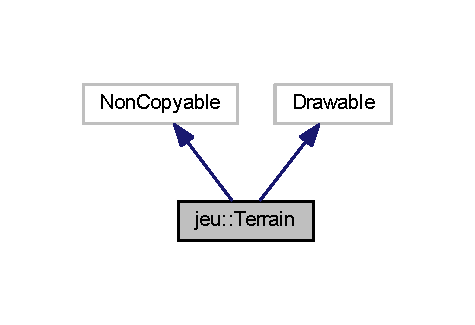
\includegraphics[width=228pt]{classjeu_1_1_terrain__inherit__graph}
\end{center}
\end{figure}


Graphe de collaboration de jeu\+:\+:Terrain\+:\nopagebreak
\begin{figure}[H]
\begin{center}
\leavevmode
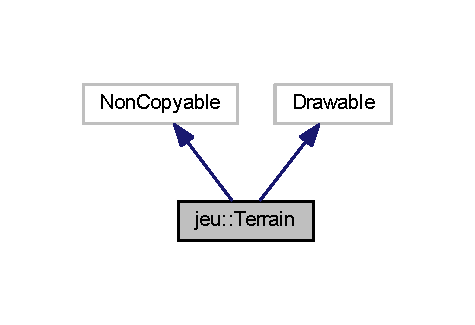
\includegraphics[width=228pt]{classjeu_1_1_terrain__coll__graph}
\end{center}
\end{figure}
\subsection*{Fonctions membres publiques}
\begin{DoxyCompactItemize}
\item 
void \hyperlink{classjeu_1_1_terrain_a863ec2c8050a5484b95fbb9e012e616e}{set\+Index\+Etage\+Courant} (std\+::size\+\_\+t val)
\begin{DoxyCompactList}\small\item\em $<$ Definir m\+\_\+index\+Etage\+Courant \end{DoxyCompactList}\item 
std\+::size\+\_\+t \hyperlink{classjeu_1_1_terrain_a044b5cdbffba772339cf9078120afd4f}{get\+Index\+Etage\+Courant} () const 
\begin{DoxyCompactList}\small\item\em Acceder � m\+\_\+index\+Etage\+Courant. \end{DoxyCompactList}\item 
void \hyperlink{classjeu_1_1_terrain_a720ed1fa9ef9cc785a4d84fff3ea6a3f}{set\+Taille} (sf\+::\+Vector2i val)
\begin{DoxyCompactList}\small\item\em Definir m\+\_\+taille. \end{DoxyCompactList}\item 
sf\+::\+Vector2i \hyperlink{classjeu_1_1_terrain_ae90b77e2d23cd2087df1c15bb23106f9}{get\+Taille} () const 
\begin{DoxyCompactList}\small\item\em Acceder � m\+\_\+taille. \end{DoxyCompactList}\item 
\hyperlink{classjeu_1_1_terrain_ae4cf297206eccab9d9b119ca34a547ad}{Terrain} ()
\begin{DoxyCompactList}\small\item\em Constructeur par d�faut. \end{DoxyCompactList}\item 
void \hyperlink{classjeu_1_1_terrain_acce6a8d053bbb70e22b6749b79cfd3b0}{generer\+Etages} (int seed=123456)
\begin{DoxyCompactList}\small\item\em Gen�re les differents �tages du terrain. \end{DoxyCompactList}\item 
void \hyperlink{classjeu_1_1_terrain_a43df1b4f47b831a2d944964ccda6e82e}{initialiser} ()
\begin{DoxyCompactList}\small\item\em Vide la liste des �tages, vide le terrain. \end{DoxyCompactList}\item 
virtual void \hyperlink{classjeu_1_1_terrain_a53fbaab5a7f98ee71569718de18f1a57}{draw} (sf\+::\+Render\+Target \&target, sf\+::\+Render\+States states) const 
\begin{DoxyCompactList}\small\item\em La fonction de dessin S\+F\+ML. Dessine l\textquotesingle{}�tage courant. \end{DoxyCompactList}\end{DoxyCompactItemize}


\subsection{Description détaillée}
Le terrain est le champs d\textquotesingle{}�volution des fourmis et autres �l�ments du biome. Compos� de plusieurs �tages ( 2? ou 3? ), il est repr�sent� en 2D avec une profondeur repr�sentant les �tages. Le "tilemap\textquotesingle{} est au niveau du pixel. 

\subsection{Documentation des constructeurs et destructeur}
\index{jeu\+::\+Terrain@{jeu\+::\+Terrain}!Terrain@{Terrain}}
\index{Terrain@{Terrain}!jeu\+::\+Terrain@{jeu\+::\+Terrain}}
\subsubsection[{\texorpdfstring{Terrain()}{Terrain()}}]{\setlength{\rightskip}{0pt plus 5cm}jeu\+::\+Terrain\+::\+Terrain (
\begin{DoxyParamCaption}
{}
\end{DoxyParamCaption}
)}\hypertarget{classjeu_1_1_terrain_ae4cf297206eccab9d9b119ca34a547ad}{}\label{classjeu_1_1_terrain_ae4cf297206eccab9d9b119ca34a547ad}


Constructeur par d�faut. 



\subsection{Documentation des fonctions membres}
\index{jeu\+::\+Terrain@{jeu\+::\+Terrain}!draw@{draw}}
\index{draw@{draw}!jeu\+::\+Terrain@{jeu\+::\+Terrain}}
\subsubsection[{\texorpdfstring{draw(sf\+::\+Render\+Target \&target, sf\+::\+Render\+States states) const }{draw(sf::RenderTarget &target, sf::RenderStates states) const }}]{\setlength{\rightskip}{0pt plus 5cm}virtual void jeu\+::\+Terrain\+::draw (
\begin{DoxyParamCaption}
\item[{sf\+::\+Render\+Target \&}]{target, }
\item[{sf\+::\+Render\+States}]{states}
\end{DoxyParamCaption}
) const\hspace{0.3cm}{\ttfamily [virtual]}}\hypertarget{classjeu_1_1_terrain_a53fbaab5a7f98ee71569718de18f1a57}{}\label{classjeu_1_1_terrain_a53fbaab5a7f98ee71569718de18f1a57}


La fonction de dessin S\+F\+ML. Dessine l\textquotesingle{}�tage courant. 


\begin{DoxyParams}{Paramètres}
{\em target} & \\
\hline
{\em states} & \\
\hline
\end{DoxyParams}
\index{jeu\+::\+Terrain@{jeu\+::\+Terrain}!generer\+Etages@{generer\+Etages}}
\index{generer\+Etages@{generer\+Etages}!jeu\+::\+Terrain@{jeu\+::\+Terrain}}
\subsubsection[{\texorpdfstring{generer\+Etages(int seed=123456)}{genererEtages(int seed=123456)}}]{\setlength{\rightskip}{0pt plus 5cm}void jeu\+::\+Terrain\+::generer\+Etages (
\begin{DoxyParamCaption}
\item[{int}]{seed = {\ttfamily 123456}}
\end{DoxyParamCaption}
)}\hypertarget{classjeu_1_1_terrain_acce6a8d053bbb70e22b6749b79cfd3b0}{}\label{classjeu_1_1_terrain_acce6a8d053bbb70e22b6749b79cfd3b0}


Gen�re les differents �tages du terrain. 


\begin{DoxyParams}{Paramètres}
{\em seed} & Permet de d�finir le seed pour la g�n�ration du bruit de Perlin. \\
\hline
\end{DoxyParams}
\index{jeu\+::\+Terrain@{jeu\+::\+Terrain}!get\+Index\+Etage\+Courant@{get\+Index\+Etage\+Courant}}
\index{get\+Index\+Etage\+Courant@{get\+Index\+Etage\+Courant}!jeu\+::\+Terrain@{jeu\+::\+Terrain}}
\subsubsection[{\texorpdfstring{get\+Index\+Etage\+Courant() const }{getIndexEtageCourant() const }}]{\setlength{\rightskip}{0pt plus 5cm}std\+::size\+\_\+t jeu\+::\+Terrain\+::get\+Index\+Etage\+Courant (
\begin{DoxyParamCaption}
{}
\end{DoxyParamCaption}
) const\hspace{0.3cm}{\ttfamily [inline]}}\hypertarget{classjeu_1_1_terrain_a044b5cdbffba772339cf9078120afd4f}{}\label{classjeu_1_1_terrain_a044b5cdbffba772339cf9078120afd4f}


Acceder � m\+\_\+index\+Etage\+Courant. 

\index{jeu\+::\+Terrain@{jeu\+::\+Terrain}!get\+Taille@{get\+Taille}}
\index{get\+Taille@{get\+Taille}!jeu\+::\+Terrain@{jeu\+::\+Terrain}}
\subsubsection[{\texorpdfstring{get\+Taille() const }{getTaille() const }}]{\setlength{\rightskip}{0pt plus 5cm}sf\+::\+Vector2i jeu\+::\+Terrain\+::get\+Taille (
\begin{DoxyParamCaption}
{}
\end{DoxyParamCaption}
) const\hspace{0.3cm}{\ttfamily [inline]}}\hypertarget{classjeu_1_1_terrain_ae90b77e2d23cd2087df1c15bb23106f9}{}\label{classjeu_1_1_terrain_ae90b77e2d23cd2087df1c15bb23106f9}


Acceder � m\+\_\+taille. 

\index{jeu\+::\+Terrain@{jeu\+::\+Terrain}!initialiser@{initialiser}}
\index{initialiser@{initialiser}!jeu\+::\+Terrain@{jeu\+::\+Terrain}}
\subsubsection[{\texorpdfstring{initialiser()}{initialiser()}}]{\setlength{\rightskip}{0pt plus 5cm}void jeu\+::\+Terrain\+::initialiser (
\begin{DoxyParamCaption}
{}
\end{DoxyParamCaption}
)}\hypertarget{classjeu_1_1_terrain_a43df1b4f47b831a2d944964ccda6e82e}{}\label{classjeu_1_1_terrain_a43df1b4f47b831a2d944964ccda6e82e}


Vide la liste des �tages, vide le terrain. 

\index{jeu\+::\+Terrain@{jeu\+::\+Terrain}!set\+Index\+Etage\+Courant@{set\+Index\+Etage\+Courant}}
\index{set\+Index\+Etage\+Courant@{set\+Index\+Etage\+Courant}!jeu\+::\+Terrain@{jeu\+::\+Terrain}}
\subsubsection[{\texorpdfstring{set\+Index\+Etage\+Courant(std\+::size\+\_\+t val)}{setIndexEtageCourant(std::size_t val)}}]{\setlength{\rightskip}{0pt plus 5cm}void jeu\+::\+Terrain\+::set\+Index\+Etage\+Courant (
\begin{DoxyParamCaption}
\item[{std\+::size\+\_\+t}]{val}
\end{DoxyParamCaption}
)\hspace{0.3cm}{\ttfamily [inline]}}\hypertarget{classjeu_1_1_terrain_a863ec2c8050a5484b95fbb9e012e616e}{}\label{classjeu_1_1_terrain_a863ec2c8050a5484b95fbb9e012e616e}


$<$ Definir m\+\_\+index\+Etage\+Courant 

\index{jeu\+::\+Terrain@{jeu\+::\+Terrain}!set\+Taille@{set\+Taille}}
\index{set\+Taille@{set\+Taille}!jeu\+::\+Terrain@{jeu\+::\+Terrain}}
\subsubsection[{\texorpdfstring{set\+Taille(sf\+::\+Vector2i val)}{setTaille(sf::Vector2i val)}}]{\setlength{\rightskip}{0pt plus 5cm}void jeu\+::\+Terrain\+::set\+Taille (
\begin{DoxyParamCaption}
\item[{sf\+::\+Vector2i}]{val}
\end{DoxyParamCaption}
)\hspace{0.3cm}{\ttfamily [inline]}}\hypertarget{classjeu_1_1_terrain_a720ed1fa9ef9cc785a4d84fff3ea6a3f}{}\label{classjeu_1_1_terrain_a720ed1fa9ef9cc785a4d84fff3ea6a3f}


Definir m\+\_\+taille. 



La documentation de cette classe a été générée à partir du fichier suivant \+:\begin{DoxyCompactItemize}
\item 
C\+:/\+Users/kris/\+One\+Drive/recherche Biome/01 -\/ code/code/include/jeu/\hyperlink{_terrain_8h}{Terrain.\+h}\end{DoxyCompactItemize}

\hypertarget{classgui_1_1_vue}{}\section{Référence de la classe gui\+:\+:Vue}
\label{classgui_1_1_vue}\index{gui\+::\+Vue@{gui\+::\+Vue}}


Une vue S\+F\+ML.  




{\ttfamily \#include $<$Vue.\+h$>$}



Graphe d\textquotesingle{}héritage de gui\+:\+:Vue\+:\nopagebreak
\begin{figure}[H]
\begin{center}
\leavevmode
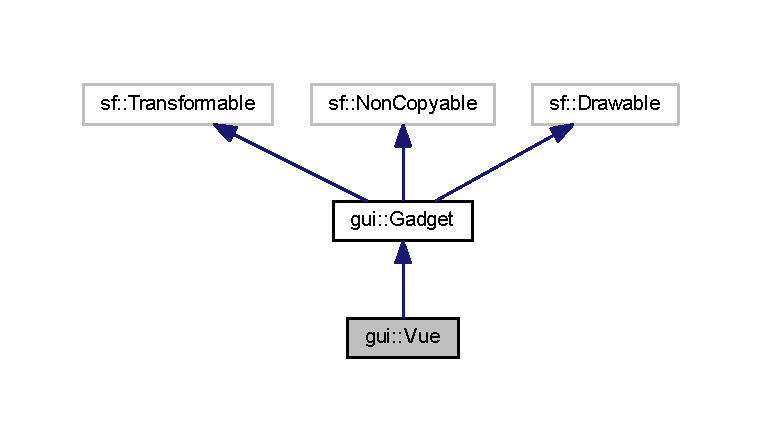
\includegraphics[width=350pt]{classgui_1_1_vue__inherit__graph}
\end{center}
\end{figure}


Graphe de collaboration de gui\+:\+:Vue\+:\nopagebreak
\begin{figure}[H]
\begin{center}
\leavevmode
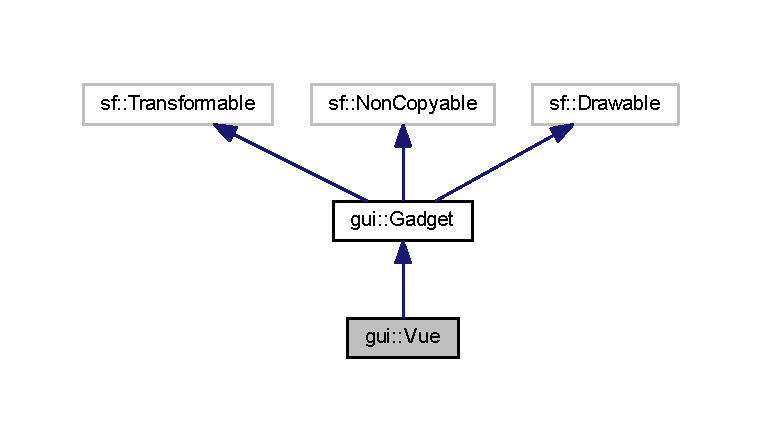
\includegraphics[width=350pt]{classgui_1_1_vue__coll__graph}
\end{center}
\end{figure}
\subsection*{Fonctions membres publiques}
\begin{DoxyCompactItemize}
\item 
void \hyperlink{classgui_1_1_vue_ad7dd41adb1ed9162e2cd9eabc27b0767}{traiter\+Evenements} (sf\+::\+Event evenement)
\begin{DoxyCompactList}\small\item\em Traitement des �venements clavier ou souris. \end{DoxyCompactList}\item 
void \hyperlink{classgui_1_1_vue_aa1d213828908722d9a5a054fcd494ef1}{actualiser} ()
\begin{DoxyCompactList}\small\item\em Actualiser les �l�ments de l\textquotesingle{}interface. \end{DoxyCompactList}\item 
virtual void \hyperlink{classgui_1_1_vue_a1439e18d8ba169399248085867528f26}{draw} (sf\+::\+Render\+Target \&target, sf\+::\+Render\+States states) const 
\begin{DoxyCompactList}\small\item\em Dessine tout les �l�ments de l\textquotesingle{}interface. \end{DoxyCompactList}\end{DoxyCompactItemize}


\subsection{Description détaillée}
Une vue S\+F\+ML. 

\subsection{Documentation des fonctions membres}
\index{gui\+::\+Vue@{gui\+::\+Vue}!actualiser@{actualiser}}
\index{actualiser@{actualiser}!gui\+::\+Vue@{gui\+::\+Vue}}
\subsubsection[{\texorpdfstring{actualiser()}{actualiser()}}]{\setlength{\rightskip}{0pt plus 5cm}void gui\+::\+Vue\+::actualiser (
\begin{DoxyParamCaption}
{}
\end{DoxyParamCaption}
)}\hypertarget{classgui_1_1_vue_aa1d213828908722d9a5a054fcd494ef1}{}\label{classgui_1_1_vue_aa1d213828908722d9a5a054fcd494ef1}


Actualiser les �l�ments de l\textquotesingle{}interface. 

\index{gui\+::\+Vue@{gui\+::\+Vue}!draw@{draw}}
\index{draw@{draw}!gui\+::\+Vue@{gui\+::\+Vue}}
\subsubsection[{\texorpdfstring{draw(sf\+::\+Render\+Target \&target, sf\+::\+Render\+States states) const }{draw(sf::RenderTarget &target, sf::RenderStates states) const }}]{\setlength{\rightskip}{0pt plus 5cm}virtual void gui\+::\+Vue\+::draw (
\begin{DoxyParamCaption}
\item[{sf\+::\+Render\+Target \&}]{target, }
\item[{sf\+::\+Render\+States}]{states}
\end{DoxyParamCaption}
) const\hspace{0.3cm}{\ttfamily [virtual]}}\hypertarget{classgui_1_1_vue_a1439e18d8ba169399248085867528f26}{}\label{classgui_1_1_vue_a1439e18d8ba169399248085867528f26}


Dessine tout les �l�ments de l\textquotesingle{}interface. 


\begin{DoxyParams}{Paramètres}
{\em target} & \\
\hline
{\em states} & \\
\hline
\end{DoxyParams}


Réimplémentée à partir de \hyperlink{classgui_1_1_gadget_a57b0c75601c7f6e0d43370013ae8c111}{gui\+::\+Gadget}.

\index{gui\+::\+Vue@{gui\+::\+Vue}!traiter\+Evenements@{traiter\+Evenements}}
\index{traiter\+Evenements@{traiter\+Evenements}!gui\+::\+Vue@{gui\+::\+Vue}}
\subsubsection[{\texorpdfstring{traiter\+Evenements(sf\+::\+Event evenement)}{traiterEvenements(sf::Event evenement)}}]{\setlength{\rightskip}{0pt plus 5cm}void gui\+::\+Vue\+::traiter\+Evenements (
\begin{DoxyParamCaption}
\item[{sf\+::\+Event}]{evenement}
\end{DoxyParamCaption}
)}\hypertarget{classgui_1_1_vue_ad7dd41adb1ed9162e2cd9eabc27b0767}{}\label{classgui_1_1_vue_ad7dd41adb1ed9162e2cd9eabc27b0767}


Traitement des �venements clavier ou souris. 


\begin{DoxyParams}{Paramètres}
{\em evenement} & L\textquotesingle{}�venemnt � tratier. \\
\hline
\end{DoxyParams}


La documentation de cette classe a été générée à partir du fichier suivant \+:\begin{DoxyCompactItemize}
\item 
C\+:/\+Users/kris/\+One\+Drive/recherche Biome/01 -\/ code/code/include/gui/\hyperlink{_vue_8h}{Vue.\+h}\end{DoxyCompactItemize}

\chapter{Documentation des fichiers}
\hypertarget{_application_8h}{}\section{Référence du fichier C\+:/\+Users/kris/\+One\+Drive/recherche Biome/01 -\/ code/code/include/appli/\+Application.h}
\label{_application_8h}\index{C\+:/\+Users/kris/\+One\+Drive/recherche Biome/01 -\/ code/code/include/appli/\+Application.\+h@{C\+:/\+Users/kris/\+One\+Drive/recherche Biome/01 -\/ code/code/include/appli/\+Application.\+h}}


La classe principale du programme.  


{\ttfamily \#include $<$appli/\+Ecran.\+h$>$}\\*
{\ttfamily \#include $<$appli/\+Gestion\+\_\+ecrans.\+h$>$}\\*
{\ttfamily \#include $<$S\+F\+M\+L/\+Graphics.\+hpp$>$}\\*
{\ttfamily \#include $<$vector$>$}\\*
Graphe des dépendances par inclusion de Application.\+h\+:\nopagebreak
\begin{figure}[H]
\begin{center}
\leavevmode
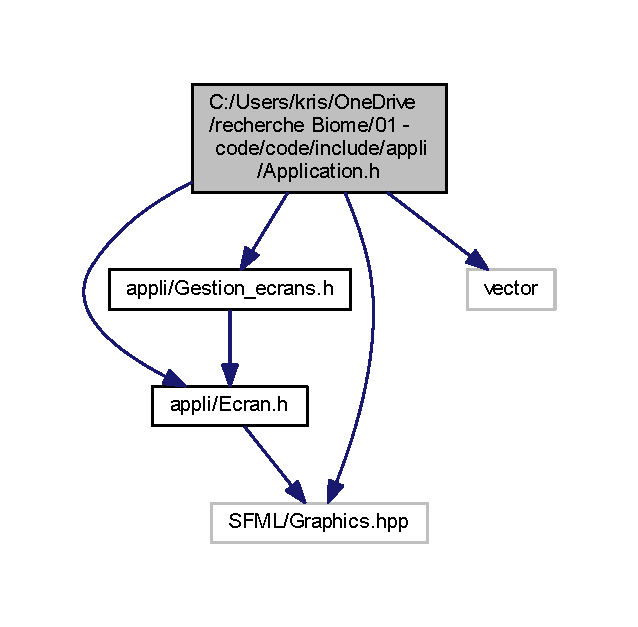
\includegraphics[width=306pt]{_application_8h__incl}
\end{center}
\end{figure}
Ce graphe montre quels fichiers incluent directement ou indirectement ce fichier \+:\nopagebreak
\begin{figure}[H]
\begin{center}
\leavevmode
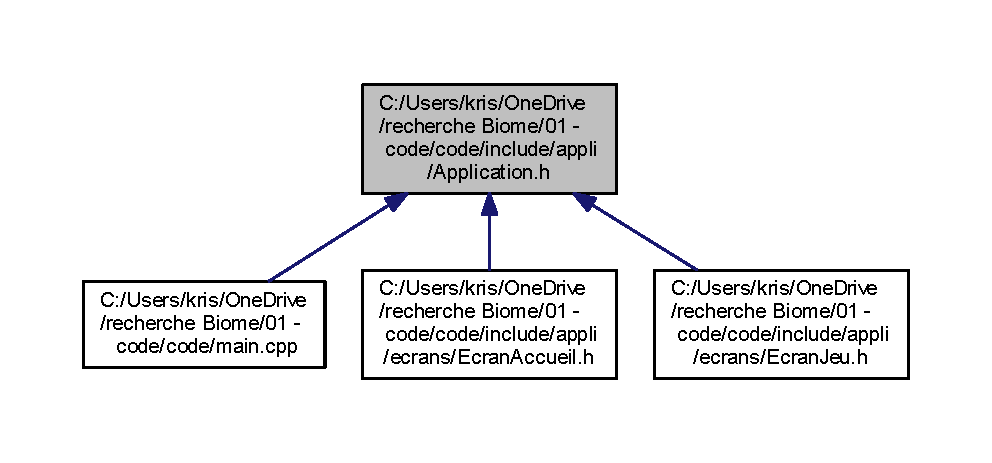
\includegraphics[width=350pt]{_application_8h__dep__incl}
\end{center}
\end{figure}
\subsection*{Classes}
\begin{DoxyCompactItemize}
\item 
class \hyperlink{classapp_1_1_application}{app\+::\+Application}
\begin{DoxyCompactList}\small\item\em La classe de base du programme. \end{DoxyCompactList}\end{DoxyCompactItemize}
\subsection*{Espaces de nommage}
\begin{DoxyCompactItemize}
\item 
 \hyperlink{namespaceapp}{app}
\end{DoxyCompactItemize}


\subsection{Description détaillée}
La classe principale du programme. 

\begin{DoxyAuthor}{Auteur}
Christophe Pages 
\end{DoxyAuthor}
\begin{DoxyVersion}{Version}
0.\+1 
\end{DoxyVersion}
\begin{DoxyDate}{Date}
2015
\end{DoxyDate}
Programme minimal g�rant differents �crans (intro, accueil, jeu, options...) 
\hypertarget{_config_8h}{}\section{Référence du fichier C\+:/\+Users/kris/\+One\+Drive/recherche Biome/01 -\/ code/code/include/appli/\+Config.h}
\label{_config_8h}\index{C\+:/\+Users/kris/\+One\+Drive/recherche Biome/01 -\/ code/code/include/appli/\+Config.\+h@{C\+:/\+Users/kris/\+One\+Drive/recherche Biome/01 -\/ code/code/include/appli/\+Config.\+h}}
{\ttfamily \#include $<$S\+F\+M\+L/\+Graphics.\+hpp$>$}\\*
{\ttfamily \#include $<$map$>$}\\*
{\ttfamily \#include $<$memory$>$}\\*
{\ttfamily \#include $<$gui/\+Gui.\+h$>$}\\*
Graphe des dépendances par inclusion de Config.\+h\+:\nopagebreak
\begin{figure}[H]
\begin{center}
\leavevmode
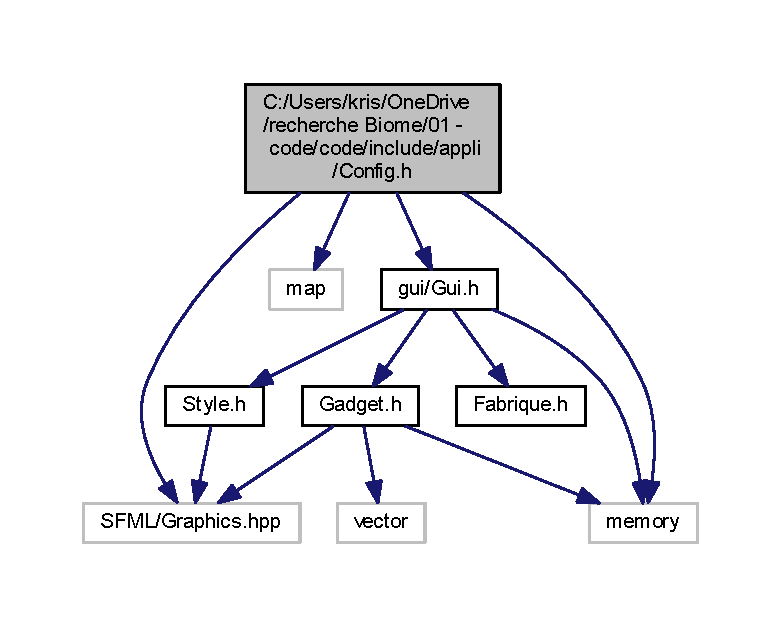
\includegraphics[width=350pt]{_config_8h__incl}
\end{center}
\end{figure}
\subsection*{Classes}
\begin{DoxyCompactItemize}
\item 
class \hyperlink{classapp_1_1_config}{app\+::\+Config}
\begin{DoxyCompactList}\small\item\em Contient les différents éléments de Configuration de l\textquotesingle{}application. \end{DoxyCompactList}\end{DoxyCompactItemize}
\subsection*{Espaces de nommage}
\begin{DoxyCompactItemize}
\item 
 \hyperlink{namespaceapp}{app}
\end{DoxyCompactItemize}

\hypertarget{_ecran_8h}{}\section{Référence du fichier C\+:/\+Users/kris/\+One\+Drive/recherche Biome/01 -\/ code/code/include/appli/\+Ecran.h}
\label{_ecran_8h}\index{C\+:/\+Users/kris/\+One\+Drive/recherche Biome/01 -\/ code/code/include/appli/\+Ecran.\+h@{C\+:/\+Users/kris/\+One\+Drive/recherche Biome/01 -\/ code/code/include/appli/\+Ecran.\+h}}
{\ttfamily \#include $<$S\+F\+M\+L/\+Graphics.\+hpp$>$}\\*
Graphe des dépendances par inclusion de Ecran.\+h\+:\nopagebreak
\begin{figure}[H]
\begin{center}
\leavevmode
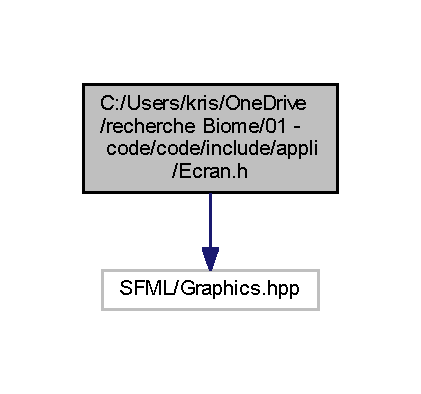
\includegraphics[width=202pt]{_ecran_8h__incl}
\end{center}
\end{figure}
Ce graphe montre quels fichiers incluent directement ou indirectement ce fichier \+:\nopagebreak
\begin{figure}[H]
\begin{center}
\leavevmode
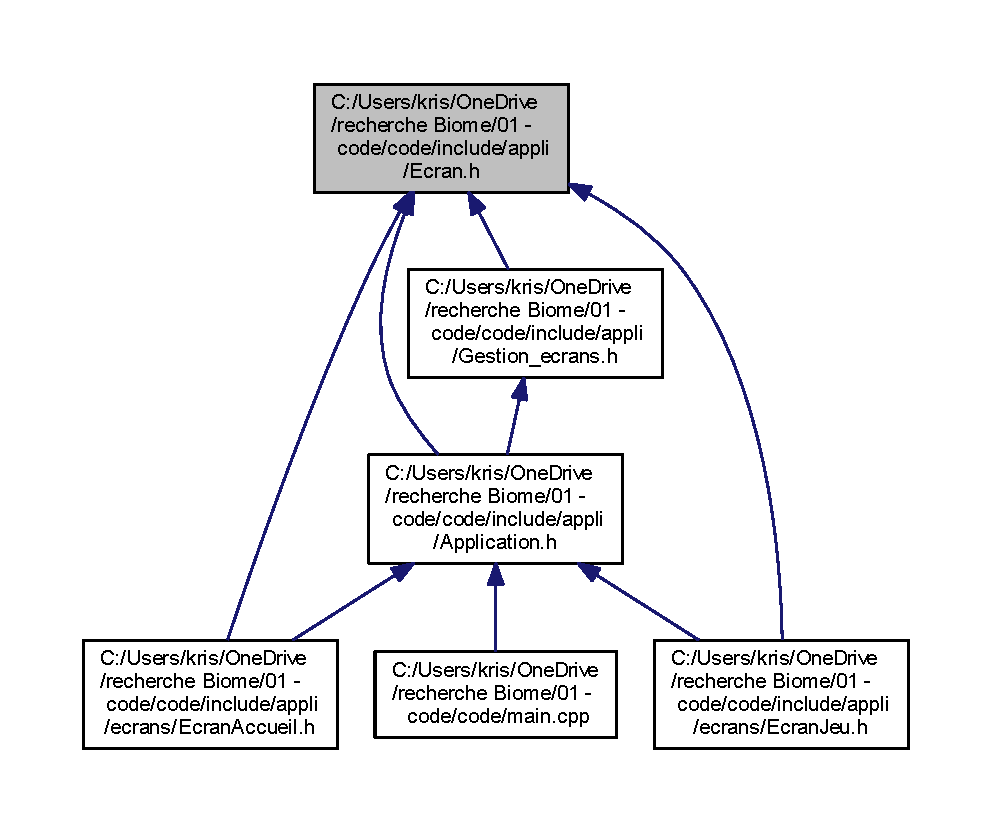
\includegraphics[width=350pt]{_ecran_8h__dep__incl}
\end{center}
\end{figure}
\subsection*{Classes}
\begin{DoxyCompactItemize}
\item 
class \hyperlink{classapp_1_1_ecran}{app\+::\+Ecran}
\begin{DoxyCompactList}\small\item\em La classe virtuelle communues aux �crans. \end{DoxyCompactList}\end{DoxyCompactItemize}
\subsection*{Espaces de nommage}
\begin{DoxyCompactItemize}
\item 
 \hyperlink{namespaceapp}{app}
\end{DoxyCompactItemize}

\hypertarget{_ecran_accueil_8h}{}\section{Référence du fichier C\+:/\+Users/kris/\+One\+Drive/recherche Biome/01 -\/ code/code/include/appli/ecrans/\+Ecran\+Accueil.h}
\label{_ecran_accueil_8h}\index{C\+:/\+Users/kris/\+One\+Drive/recherche Biome/01 -\/ code/code/include/appli/ecrans/\+Ecran\+Accueil.\+h@{C\+:/\+Users/kris/\+One\+Drive/recherche Biome/01 -\/ code/code/include/appli/ecrans/\+Ecran\+Accueil.\+h}}
{\ttfamily \#include $<$S\+F\+M\+L/\+Graphics.\+hpp$>$}\\*
{\ttfamily \#include $<$appli/\+Ecran.\+h$>$}\\*
{\ttfamily \#include $<$appli/\+Application.\+h$>$}\\*
Graphe des dépendances par inclusion de Ecran\+Accueil.\+h\+:\nopagebreak
\begin{figure}[H]
\begin{center}
\leavevmode
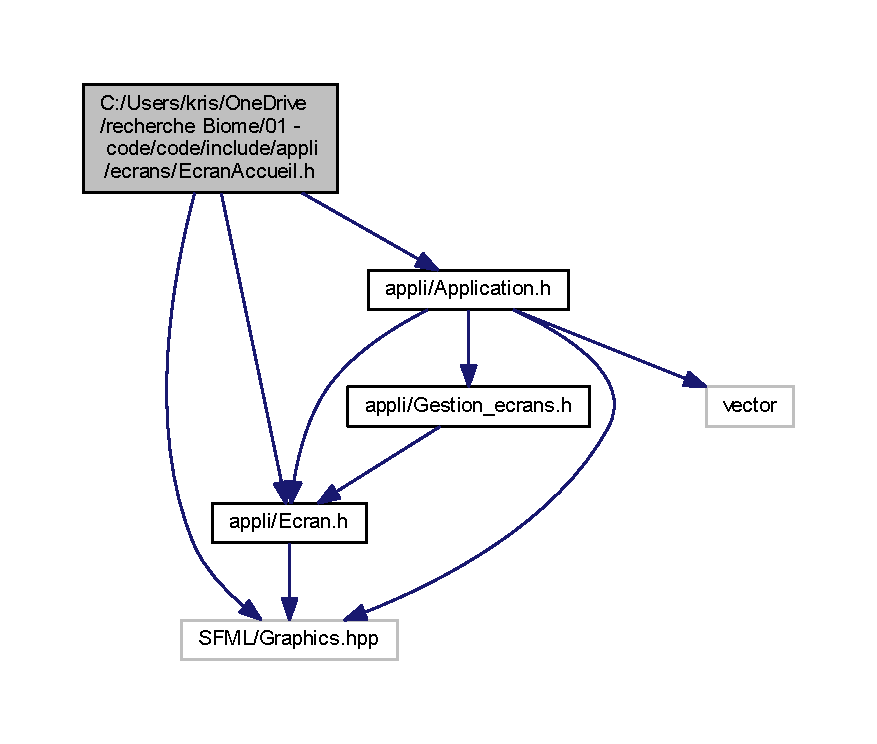
\includegraphics[width=350pt]{_ecran_accueil_8h__incl}
\end{center}
\end{figure}
\subsection*{Classes}
\begin{DoxyCompactItemize}
\item 
class \hyperlink{classapp_1_1_ecran_accueil}{app\+::\+Ecran\+Accueil}
\begin{DoxyCompactList}\small\item\em \hyperlink{classapp_1_1_ecran}{Ecran} de démonstration. \end{DoxyCompactList}\end{DoxyCompactItemize}
\subsection*{Espaces de nommage}
\begin{DoxyCompactItemize}
\item 
 \hyperlink{namespaceapp}{app}
\end{DoxyCompactItemize}

\hypertarget{_ecran_jeu_8h}{}\section{Référence du fichier C\+:/\+Users/kris/\+One\+Drive/recherche Biome/01 -\/ code/code/include/appli/ecrans/\+Ecran\+Jeu.h}
\label{_ecran_jeu_8h}\index{C\+:/\+Users/kris/\+One\+Drive/recherche Biome/01 -\/ code/code/include/appli/ecrans/\+Ecran\+Jeu.\+h@{C\+:/\+Users/kris/\+One\+Drive/recherche Biome/01 -\/ code/code/include/appli/ecrans/\+Ecran\+Jeu.\+h}}
{\ttfamily \#include $<$S\+F\+M\+L/\+Graphics.\+hpp$>$}\\*
{\ttfamily \#include $<$appli/\+Ecran.\+h$>$}\\*
{\ttfamily \#include $<$appli/\+Application.\+h$>$}\\*
{\ttfamily \#include \char`\"{}jeu/\+Jeu.\+h\char`\"{}}\\*
Graphe des dépendances par inclusion de Ecran\+Jeu.\+h\+:\nopagebreak
\begin{figure}[H]
\begin{center}
\leavevmode
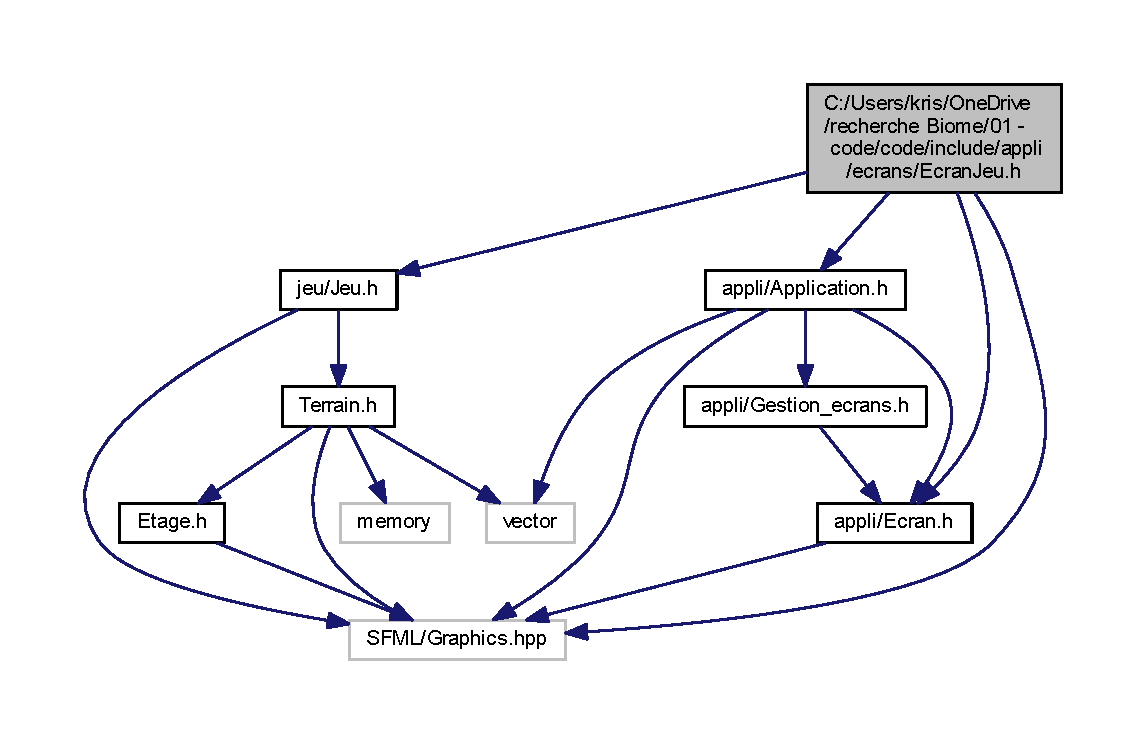
\includegraphics[width=350pt]{_ecran_jeu_8h__incl}
\end{center}
\end{figure}
\subsection*{Classes}
\begin{DoxyCompactItemize}
\item 
class \hyperlink{classapp_1_1_ecran_jeu}{app\+::\+Ecran\+Jeu}
\begin{DoxyCompactList}\small\item\em \hyperlink{classapp_1_1_ecran}{Ecran} de jeu. \end{DoxyCompactList}\end{DoxyCompactItemize}
\subsection*{Espaces de nommage}
\begin{DoxyCompactItemize}
\item 
 \hyperlink{namespaceapp}{app}
\end{DoxyCompactItemize}

\hypertarget{_gestion__ecrans_8h}{}\section{Référence du fichier C\+:/\+Users/kris/\+One\+Drive/recherche Biome/01 -\/ code/code/include/appli/\+Gestion\+\_\+ecrans.h}
\label{_gestion__ecrans_8h}\index{C\+:/\+Users/kris/\+One\+Drive/recherche Biome/01 -\/ code/code/include/appli/\+Gestion\+\_\+ecrans.\+h@{C\+:/\+Users/kris/\+One\+Drive/recherche Biome/01 -\/ code/code/include/appli/\+Gestion\+\_\+ecrans.\+h}}
{\ttfamily \#include $<$appli/\+Ecran.\+h$>$}\\*
Graphe des dépendances par inclusion de Gestion\+\_\+ecrans.\+h\+:\nopagebreak
\begin{figure}[H]
\begin{center}
\leavevmode
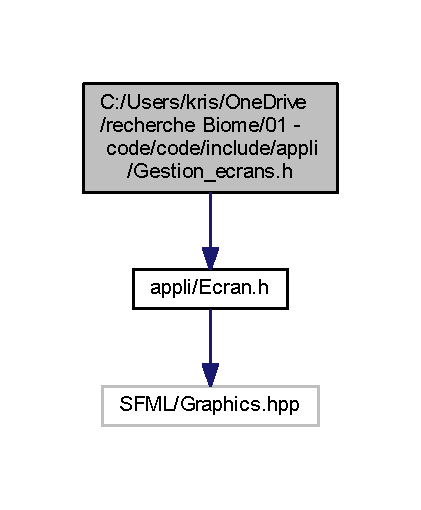
\includegraphics[width=202pt]{_gestion__ecrans_8h__incl}
\end{center}
\end{figure}
Ce graphe montre quels fichiers incluent directement ou indirectement ce fichier \+:\nopagebreak
\begin{figure}[H]
\begin{center}
\leavevmode
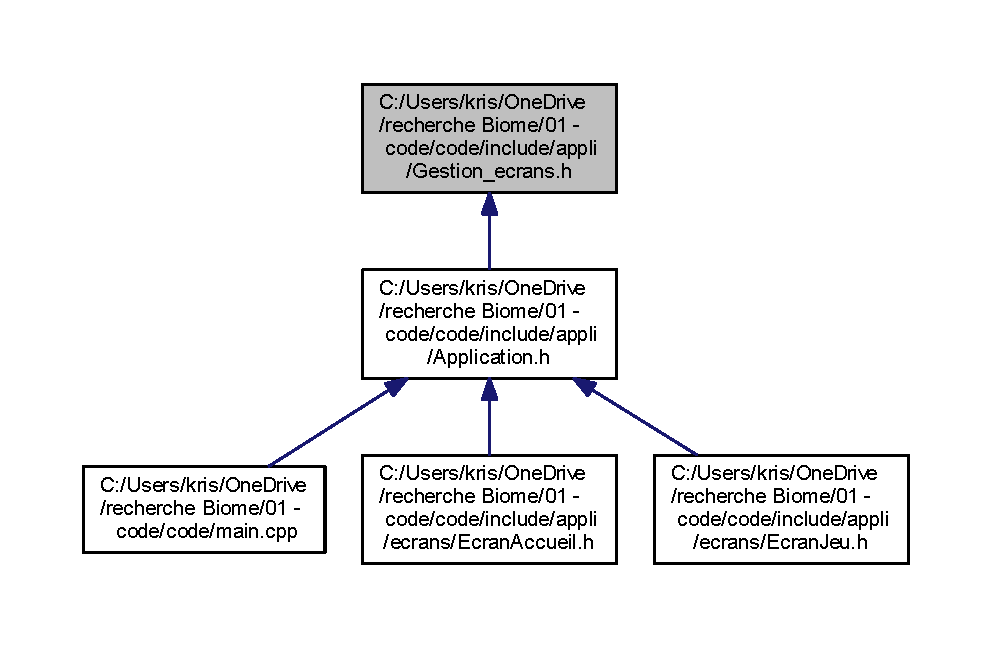
\includegraphics[width=350pt]{_gestion__ecrans_8h__dep__incl}
\end{center}
\end{figure}
\subsection*{Classes}
\begin{DoxyCompactItemize}
\item 
class \hyperlink{classapp_1_1_gestion__ecrans}{app\+::\+Gestion\+\_\+ecrans}
\begin{DoxyCompactList}\small\item\em Gestionnaire des �crans. \end{DoxyCompactList}\end{DoxyCompactItemize}
\subsection*{Espaces de nommage}
\begin{DoxyCompactItemize}
\item 
 \hyperlink{namespaceapp}{app}
\end{DoxyCompactItemize}

\hypertarget{_resource_mgr_8h}{}\section{Référence du fichier C\+:/\+Users/kris/\+One\+Drive/recherche Biome/01 -\/ code/code/include/appli/\+Resource\+Mgr.h}
\label{_resource_mgr_8h}\index{C\+:/\+Users/kris/\+One\+Drive/recherche Biome/01 -\/ code/code/include/appli/\+Resource\+Mgr.\+h@{C\+:/\+Users/kris/\+One\+Drive/recherche Biome/01 -\/ code/code/include/appli/\+Resource\+Mgr.\+h}}
{\ttfamily \#include $<$unordered\+\_\+map$>$}\\*
{\ttfamily \#include $<$memory$>$}\\*
{\ttfamily \#include $<$stdexcept$>$}\\*
{\ttfamily \#include $<$S\+F\+M\+L/\+Graphics.\+hpp$>$}\\*
{\ttfamily \#include $<$S\+F\+M\+L/audio.\+hpp$>$}\\*
{\ttfamily \#include $<$Resource\+Mgr.\+inl$>$}\\*
Graphe des dépendances par inclusion de Resource\+Mgr.\+h\+:\nopagebreak
\begin{figure}[H]
\begin{center}
\leavevmode
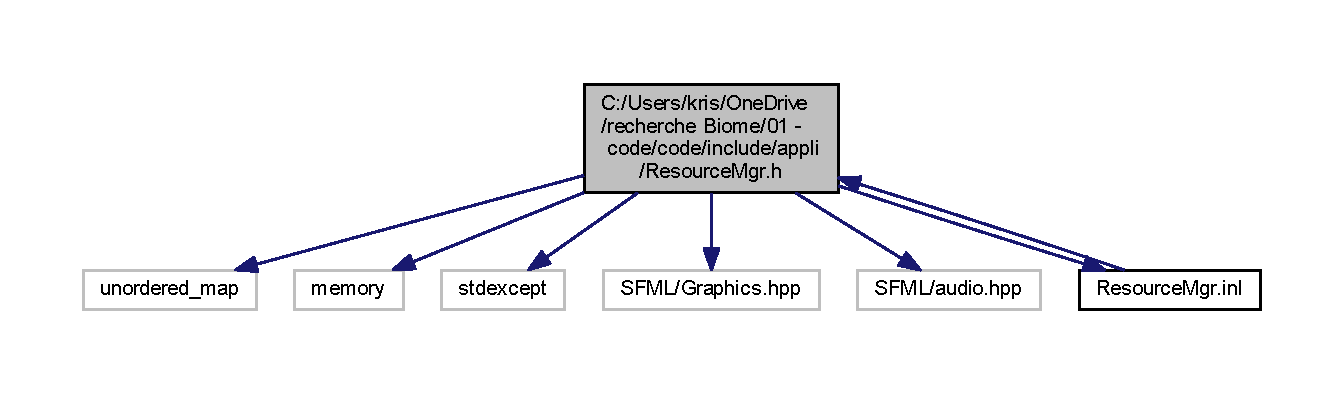
\includegraphics[width=350pt]{_resource_mgr_8h__incl}
\end{center}
\end{figure}
Ce graphe montre quels fichiers incluent directement ou indirectement ce fichier \+:\nopagebreak
\begin{figure}[H]
\begin{center}
\leavevmode
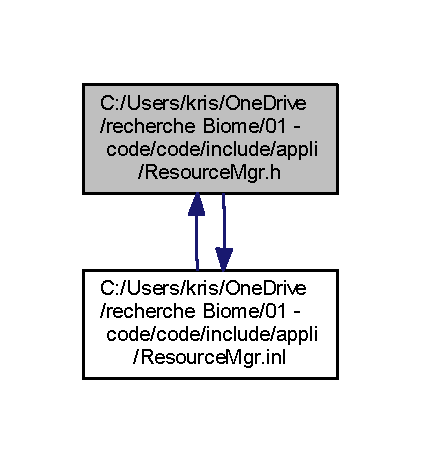
\includegraphics[width=202pt]{_resource_mgr_8h__dep__incl}
\end{center}
\end{figure}
\subsection*{Classes}
\begin{DoxyCompactItemize}
\item 
class \hyperlink{classapp_1_1_resource_mgr}{app\+::\+Resource\+Mgr$<$ R\+E\+S\+O\+U\+R\+C\+E, I\+D\+E\+N\+T\+I\+F\+I\+A\+N\+T $>$}
\begin{DoxyCompactList}\small\item\em Manager de ressource (polices, images). \end{DoxyCompactList}\item 
class \hyperlink{classapp_1_1_resource_mgr_3_01sf_1_1_music_00_01_i_d_e_n_t_i_f_i_a_n_t_01_4}{app\+::\+Resource\+Mgr$<$ sf\+::\+Music, I\+D\+E\+N\+T\+I\+F\+I\+A\+N\+T $>$}
\begin{DoxyCompactList}\small\item\em Manager de ressource (music). \end{DoxyCompactList}\end{DoxyCompactItemize}
\subsection*{Espaces de nommage}
\begin{DoxyCompactItemize}
\item 
 \hyperlink{namespaceapp}{app}
\end{DoxyCompactItemize}

\hypertarget{_resource_mgr_8inl}{}\section{Référence du fichier C\+:/\+Users/kris/\+One\+Drive/recherche Biome/01 -\/ code/code/include/appli/\+Resource\+Mgr.inl}
\label{_resource_mgr_8inl}\index{C\+:/\+Users/kris/\+One\+Drive/recherche Biome/01 -\/ code/code/include/appli/\+Resource\+Mgr.\+inl@{C\+:/\+Users/kris/\+One\+Drive/recherche Biome/01 -\/ code/code/include/appli/\+Resource\+Mgr.\+inl}}
{\ttfamily \#include \char`\"{}Resource\+Mgr.\+h\char`\"{}}\\*
Graphe des dépendances par inclusion de Resource\+Mgr.\+inl\+:\nopagebreak
\begin{figure}[H]
\begin{center}
\leavevmode
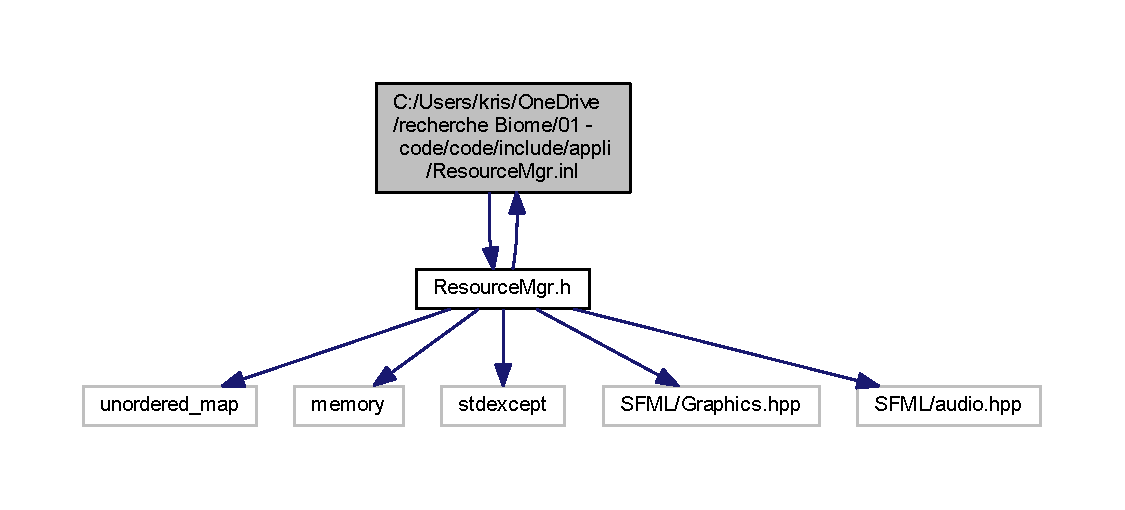
\includegraphics[width=350pt]{_resource_mgr_8inl__incl}
\end{center}
\end{figure}
Ce graphe montre quels fichiers incluent directement ou indirectement ce fichier \+:\nopagebreak
\begin{figure}[H]
\begin{center}
\leavevmode
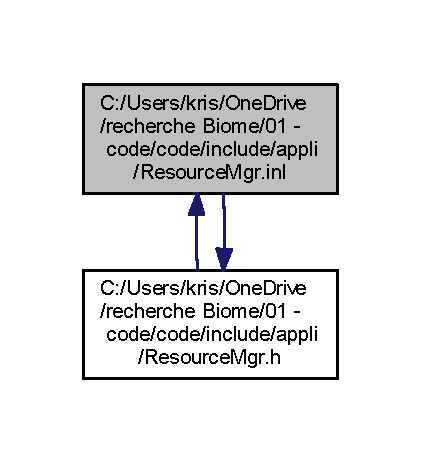
\includegraphics[width=202pt]{_resource_mgr_8inl__dep__incl}
\end{center}
\end{figure}
\subsection*{Espaces de nommage}
\begin{DoxyCompactItemize}
\item 
 \hyperlink{namespaceapp}{app}
\end{DoxyCompactItemize}

\hypertarget{_bouton_8h}{}\section{Référence du fichier C\+:/\+Users/kris/\+One\+Drive/recherche Biome/01 -\/ code/code/include/gui/\+Bouton.h}
\label{_bouton_8h}\index{C\+:/\+Users/kris/\+One\+Drive/recherche Biome/01 -\/ code/code/include/gui/\+Bouton.\+h@{C\+:/\+Users/kris/\+One\+Drive/recherche Biome/01 -\/ code/code/include/gui/\+Bouton.\+h}}
{\ttfamily \#include \char`\"{}Gadget.\+h\char`\"{}}\\*
Graphe des dépendances par inclusion de Bouton.\+h\+:\nopagebreak
\begin{figure}[H]
\begin{center}
\leavevmode
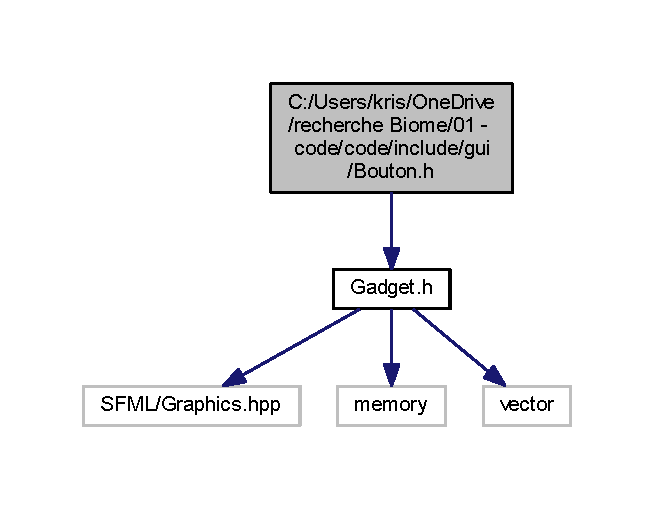
\includegraphics[width=314pt]{_bouton_8h__incl}
\end{center}
\end{figure}
\subsection*{Classes}
\begin{DoxyCompactItemize}
\item 
class \hyperlink{classgui_1_1_bouton}{gui\+::\+Bouton}
\begin{DoxyCompactList}\small\item\em Un bouton. \end{DoxyCompactList}\end{DoxyCompactItemize}
\subsection*{Espaces de nommage}
\begin{DoxyCompactItemize}
\item 
 \hyperlink{namespacegui}{gui}
\end{DoxyCompactItemize}

\hypertarget{_fabrique_8h}{}\section{Référence du fichier C\+:/\+Users/kris/\+One\+Drive/recherche Biome/01 -\/ code/code/include/gui/\+Fabrique.h}
\label{_fabrique_8h}\index{C\+:/\+Users/kris/\+One\+Drive/recherche Biome/01 -\/ code/code/include/gui/\+Fabrique.\+h@{C\+:/\+Users/kris/\+One\+Drive/recherche Biome/01 -\/ code/code/include/gui/\+Fabrique.\+h}}
Ce graphe montre quels fichiers incluent directement ou indirectement ce fichier \+:\nopagebreak
\begin{figure}[H]
\begin{center}
\leavevmode
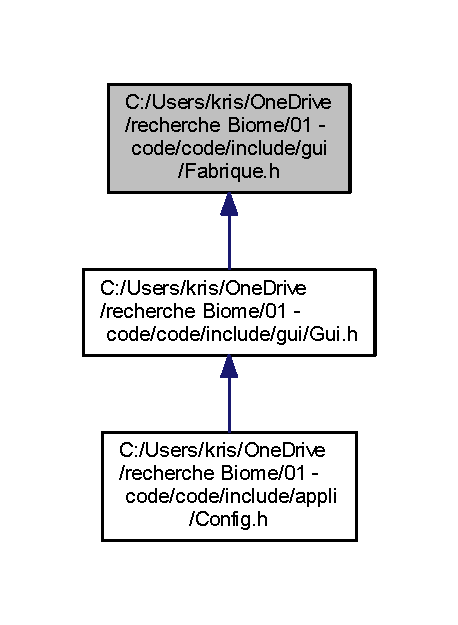
\includegraphics[width=220pt]{_fabrique_8h__dep__incl}
\end{center}
\end{figure}
\subsection*{Classes}
\begin{DoxyCompactItemize}
\item 
class \hyperlink{classgui_1_1_fabrique}{gui\+::\+Fabrique}
\begin{DoxyCompactList}\small\item\em La fabrique des gadget. \end{DoxyCompactList}\end{DoxyCompactItemize}
\subsection*{Espaces de nommage}
\begin{DoxyCompactItemize}
\item 
 \hyperlink{namespacegui}{gui}
\end{DoxyCompactItemize}

\hypertarget{_fenetre_8h}{}\section{Référence du fichier C\+:/\+Users/kris/\+One\+Drive/recherche Biome/01 -\/ code/code/include/gui/\+Fenetre.h}
\label{_fenetre_8h}\index{C\+:/\+Users/kris/\+One\+Drive/recherche Biome/01 -\/ code/code/include/gui/\+Fenetre.\+h@{C\+:/\+Users/kris/\+One\+Drive/recherche Biome/01 -\/ code/code/include/gui/\+Fenetre.\+h}}
{\ttfamily \#include \char`\"{}Gadget.\+h\char`\"{}}\\*
Graphe des dépendances par inclusion de Fenetre.\+h\+:\nopagebreak
\begin{figure}[H]
\begin{center}
\leavevmode
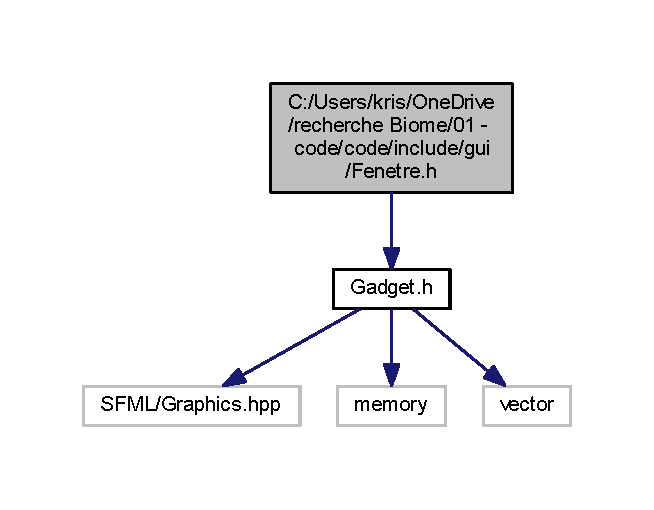
\includegraphics[width=314pt]{_fenetre_8h__incl}
\end{center}
\end{figure}
\subsection*{Classes}
\begin{DoxyCompactItemize}
\item 
class \hyperlink{classgui_1_1_fenetre}{gui\+::\+Fenetre}
\begin{DoxyCompactList}\small\item\em Une fen�tre encapsule des �l�ments d\textquotesingle{}interface. \end{DoxyCompactList}\end{DoxyCompactItemize}
\subsection*{Espaces de nommage}
\begin{DoxyCompactItemize}
\item 
 \hyperlink{namespacegui}{gui}
\end{DoxyCompactItemize}

\hypertarget{_gadget_8h}{}\section{Référence du fichier C\+:/\+Users/kris/\+One\+Drive/recherche Biome/01 -\/ code/code/include/gui/\+Gadget.h}
\label{_gadget_8h}\index{C\+:/\+Users/kris/\+One\+Drive/recherche Biome/01 -\/ code/code/include/gui/\+Gadget.\+h@{C\+:/\+Users/kris/\+One\+Drive/recherche Biome/01 -\/ code/code/include/gui/\+Gadget.\+h}}
{\ttfamily \#include $<$S\+F\+M\+L/\+Graphics.\+hpp$>$}\\*
{\ttfamily \#include $<$memory$>$}\\*
{\ttfamily \#include $<$vector$>$}\\*
Graphe des dépendances par inclusion de Gadget.\+h\+:\nopagebreak
\begin{figure}[H]
\begin{center}
\leavevmode
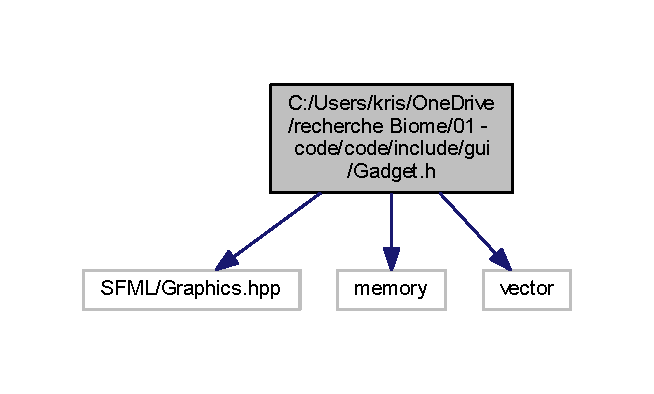
\includegraphics[width=314pt]{_gadget_8h__incl}
\end{center}
\end{figure}
Ce graphe montre quels fichiers incluent directement ou indirectement ce fichier \+:\nopagebreak
\begin{figure}[H]
\begin{center}
\leavevmode
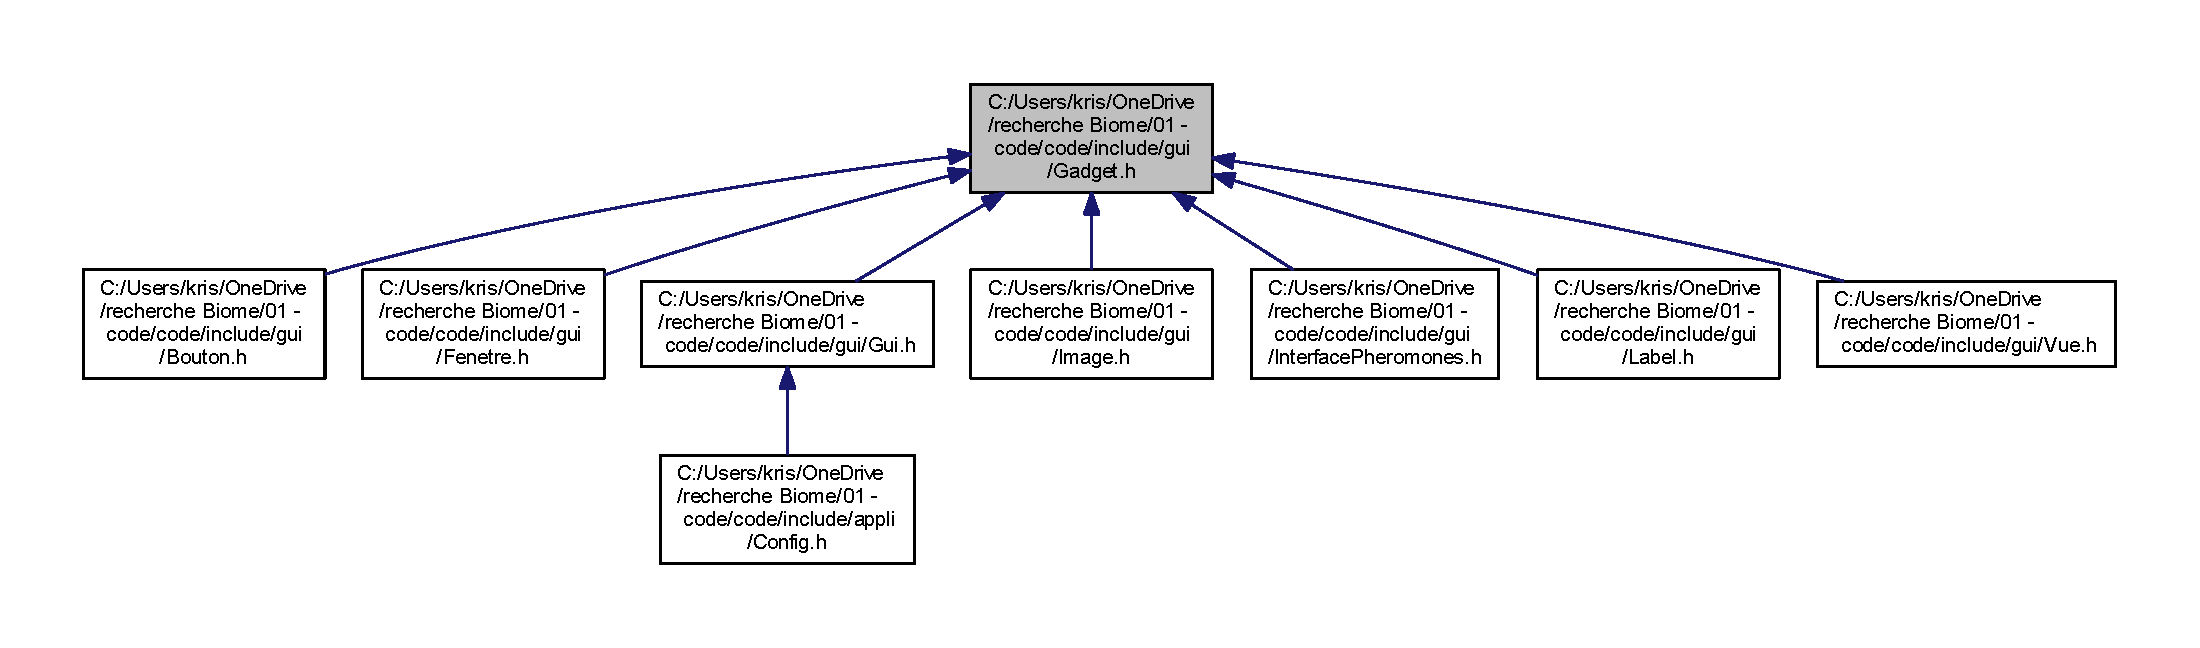
\includegraphics[width=350pt]{_gadget_8h__dep__incl}
\end{center}
\end{figure}
\subsection*{Classes}
\begin{DoxyCompactItemize}
\item 
class \hyperlink{classgui_1_1_gadget}{gui\+::\+Gadget}
\begin{DoxyCompactList}\small\item\em Un gadget est la classe abstraite des �l�ments de l\textquotesingle{}interface. \end{DoxyCompactList}\end{DoxyCompactItemize}
\subsection*{Espaces de nommage}
\begin{DoxyCompactItemize}
\item 
 \hyperlink{namespacegui}{gui}
\end{DoxyCompactItemize}

\hypertarget{_gui_8h}{}\section{Référence du fichier C\+:/\+Users/kris/\+One\+Drive/recherche Biome/01 -\/ code/code/include/gui/\+Gui.h}
\label{_gui_8h}\index{C\+:/\+Users/kris/\+One\+Drive/recherche Biome/01 -\/ code/code/include/gui/\+Gui.\+h@{C\+:/\+Users/kris/\+One\+Drive/recherche Biome/01 -\/ code/code/include/gui/\+Gui.\+h}}
{\ttfamily \#include \char`\"{}Gadget.\+h\char`\"{}}\\*
{\ttfamily \#include $<$memory$>$}\\*
{\ttfamily \#include \char`\"{}Fabrique.\+h\char`\"{}}\\*
{\ttfamily \#include \char`\"{}Style.\+h\char`\"{}}\\*
Graphe des dépendances par inclusion de Gui.\+h\+:\nopagebreak
\begin{figure}[H]
\begin{center}
\leavevmode
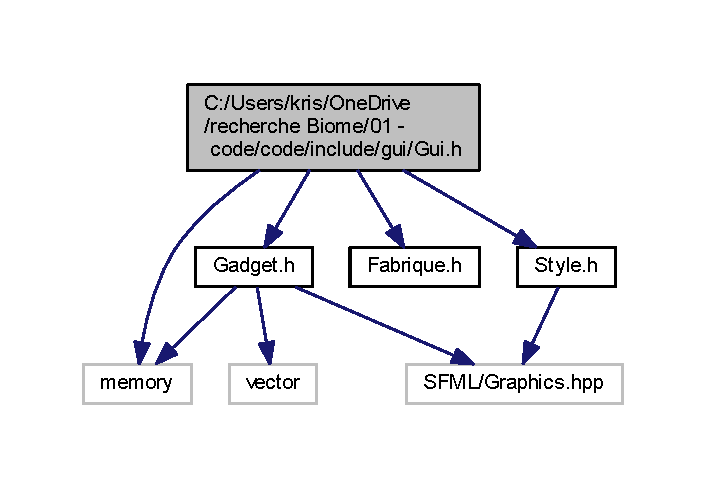
\includegraphics[width=339pt]{_gui_8h__incl}
\end{center}
\end{figure}
Ce graphe montre quels fichiers incluent directement ou indirectement ce fichier \+:\nopagebreak
\begin{figure}[H]
\begin{center}
\leavevmode
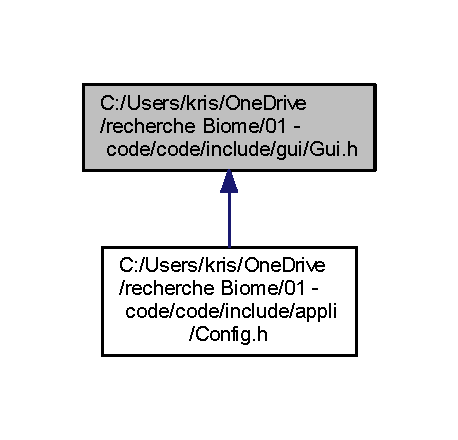
\includegraphics[width=220pt]{_gui_8h__dep__incl}
\end{center}
\end{figure}
\subsection*{Classes}
\begin{DoxyCompactItemize}
\item 
class \hyperlink{classgui_1_1_gui}{gui\+::\+Gui}
\begin{DoxyCompactList}\small\item\em Le \hyperlink{classgui_1_1_gui}{Gui} g�re l\textquotesingle{}ensemble des interactions homme-\/machine du jeu. D\textquotesingle{}un cot� un syst�me de fen�tre, boutons basique g�rant les diff�rents menus de l\textquotesingle{}appli. De l\textquotesingle{}autre, le menu ph�romones, syst�me central de l\textquotesingle{}interaction du joueur avec ses fourmis. \end{DoxyCompactList}\end{DoxyCompactItemize}
\subsection*{Espaces de nommage}
\begin{DoxyCompactItemize}
\item 
 \hyperlink{namespacegui}{gui}
\end{DoxyCompactItemize}

\hypertarget{_image_8h}{}\section{Référence du fichier C\+:/\+Users/kris/\+One\+Drive/recherche Biome/01 -\/ code/code/include/gui/\+Image.h}
\label{_image_8h}\index{C\+:/\+Users/kris/\+One\+Drive/recherche Biome/01 -\/ code/code/include/gui/\+Image.\+h@{C\+:/\+Users/kris/\+One\+Drive/recherche Biome/01 -\/ code/code/include/gui/\+Image.\+h}}
{\ttfamily \#include \char`\"{}Gadget.\+h\char`\"{}}\\*
Graphe des dépendances par inclusion de Image.\+h\+:\nopagebreak
\begin{figure}[H]
\begin{center}
\leavevmode
\includegraphics[width=314pt]{_image_8h__incl}
\end{center}
\end{figure}
\subsection*{Classes}
\begin{DoxyCompactItemize}
\item 
class \hyperlink{classgui_1_1_image}{gui\+::\+Image}
\begin{DoxyCompactList}\small\item\em Une simple image. \end{DoxyCompactList}\end{DoxyCompactItemize}
\subsection*{Espaces de nommage}
\begin{DoxyCompactItemize}
\item 
 \hyperlink{namespacegui}{gui}
\end{DoxyCompactItemize}

\hypertarget{_interface_pheromones_8h}{}\section{Référence du fichier C\+:/\+Users/kris/\+One\+Drive/recherche Biome/01 -\/ code/code/include/gui/\+Interface\+Pheromones.h}
\label{_interface_pheromones_8h}\index{C\+:/\+Users/kris/\+One\+Drive/recherche Biome/01 -\/ code/code/include/gui/\+Interface\+Pheromones.\+h@{C\+:/\+Users/kris/\+One\+Drive/recherche Biome/01 -\/ code/code/include/gui/\+Interface\+Pheromones.\+h}}
{\ttfamily \#include \char`\"{}Gadget.\+h\char`\"{}}\\*
Graphe des dépendances par inclusion de Interface\+Pheromones.\+h\+:\nopagebreak
\begin{figure}[H]
\begin{center}
\leavevmode
\includegraphics[width=314pt]{_interface_pheromones_8h__incl}
\end{center}
\end{figure}
\subsection*{Classes}
\begin{DoxyCompactItemize}
\item 
class \hyperlink{classgui_1_1_interface_pheromones}{gui\+::\+Interface\+Pheromones}
\begin{DoxyCompactList}\small\item\em L\textquotesingle{}interface des ph�romones. \end{DoxyCompactList}\end{DoxyCompactItemize}
\subsection*{Espaces de nommage}
\begin{DoxyCompactItemize}
\item 
 \hyperlink{namespacegui}{gui}
\end{DoxyCompactItemize}

\hypertarget{_label_8h}{}\section{Référence du fichier C\+:/\+Users/kris/\+One\+Drive/recherche Biome/01 -\/ code/code/include/gui/\+Label.h}
\label{_label_8h}\index{C\+:/\+Users/kris/\+One\+Drive/recherche Biome/01 -\/ code/code/include/gui/\+Label.\+h@{C\+:/\+Users/kris/\+One\+Drive/recherche Biome/01 -\/ code/code/include/gui/\+Label.\+h}}
{\ttfamily \#include \char`\"{}Gadget.\+h\char`\"{}}\\*
Graphe des dépendances par inclusion de Label.\+h\+:\nopagebreak
\begin{figure}[H]
\begin{center}
\leavevmode
\includegraphics[width=314pt]{_label_8h__incl}
\end{center}
\end{figure}
\subsection*{Classes}
\begin{DoxyCompactItemize}
\item 
class \hyperlink{classgui_1_1_label}{gui\+::\+Label}
\begin{DoxyCompactList}\small\item\em Un simple label. \end{DoxyCompactList}\end{DoxyCompactItemize}
\subsection*{Espaces de nommage}
\begin{DoxyCompactItemize}
\item 
 \hyperlink{namespacegui}{gui}
\end{DoxyCompactItemize}

\hypertarget{_style_8h}{}\section{Référence du fichier C\+:/\+Users/kris/\+One\+Drive/recherche Biome/01 -\/ code/code/include/gui/\+Style.h}
\label{_style_8h}\index{C\+:/\+Users/kris/\+One\+Drive/recherche Biome/01 -\/ code/code/include/gui/\+Style.\+h@{C\+:/\+Users/kris/\+One\+Drive/recherche Biome/01 -\/ code/code/include/gui/\+Style.\+h}}
{\ttfamily \#include $<$S\+F\+M\+L/\+Graphics.\+hpp$>$}\\*
Graphe des dépendances par inclusion de Style.\+h\+:\nopagebreak
\begin{figure}[H]
\begin{center}
\leavevmode
\includegraphics[width=196pt]{_style_8h__incl}
\end{center}
\end{figure}
Ce graphe montre quels fichiers incluent directement ou indirectement ce fichier \+:\nopagebreak
\begin{figure}[H]
\begin{center}
\leavevmode
\includegraphics[width=220pt]{_style_8h__dep__incl}
\end{center}
\end{figure}
\subsection*{Classes}
\begin{DoxyCompactItemize}
\item 
class \hyperlink{classgui_1_1_style}{gui\+::\+Style}
\begin{DoxyCompactList}\small\item\em Regroupe les couleurs, polices et style de texte de l\textquotesingle{}interface. \end{DoxyCompactList}\end{DoxyCompactItemize}
\subsection*{Espaces de nommage}
\begin{DoxyCompactItemize}
\item 
 \hyperlink{namespacegui}{gui}
\end{DoxyCompactItemize}

\hypertarget{_vue_8h}{}\section{Référence du fichier C\+:/\+Users/kris/\+One\+Drive/recherche Biome/01 -\/ code/code/include/gui/\+Vue.h}
\label{_vue_8h}\index{C\+:/\+Users/kris/\+One\+Drive/recherche Biome/01 -\/ code/code/include/gui/\+Vue.\+h@{C\+:/\+Users/kris/\+One\+Drive/recherche Biome/01 -\/ code/code/include/gui/\+Vue.\+h}}
{\ttfamily \#include \char`\"{}Gadget.\+h\char`\"{}}\\*
Graphe des dépendances par inclusion de Vue.\+h\+:\nopagebreak
\begin{figure}[H]
\begin{center}
\leavevmode
\includegraphics[width=314pt]{_vue_8h__incl}
\end{center}
\end{figure}
\subsection*{Classes}
\begin{DoxyCompactItemize}
\item 
class \hyperlink{classgui_1_1_vue}{gui\+::\+Vue}
\begin{DoxyCompactList}\small\item\em Une vue S\+F\+ML. \end{DoxyCompactList}\end{DoxyCompactItemize}
\subsection*{Espaces de nommage}
\begin{DoxyCompactItemize}
\item 
 \hyperlink{namespacegui}{gui}
\end{DoxyCompactItemize}

\hypertarget{_etage_8h}{}\section{Référence du fichier C\+:/\+Users/kris/\+One\+Drive/recherche Biome/01 -\/ code/code/include/jeu/\+Etage.h}
\label{_etage_8h}\index{C\+:/\+Users/kris/\+One\+Drive/recherche Biome/01 -\/ code/code/include/jeu/\+Etage.\+h@{C\+:/\+Users/kris/\+One\+Drive/recherche Biome/01 -\/ code/code/include/jeu/\+Etage.\+h}}
{\ttfamily \#include $<$S\+F\+M\+L/\+Graphics.\+hpp$>$}\\*
Graphe des dépendances par inclusion de Etage.\+h\+:\nopagebreak
\begin{figure}[H]
\begin{center}
\leavevmode
\includegraphics[width=196pt]{_etage_8h__incl}
\end{center}
\end{figure}
Ce graphe montre quels fichiers incluent directement ou indirectement ce fichier \+:\nopagebreak
\begin{figure}[H]
\begin{center}
\leavevmode
\includegraphics[width=220pt]{_etage_8h__dep__incl}
\end{center}
\end{figure}
\subsection*{Classes}
\begin{DoxyCompactItemize}
\item 
class \hyperlink{classjeu_1_1_etage}{jeu\+::\+Etage}
\begin{DoxyCompactList}\small\item\em Un seul �tage est visible � la fois. Compos� de sol, terre et vide. Chaque �tage g�re les collisions. \end{DoxyCompactList}\end{DoxyCompactItemize}
\subsection*{Espaces de nommage}
\begin{DoxyCompactItemize}
\item 
 \hyperlink{namespacejeu}{jeu}
\end{DoxyCompactItemize}

\hypertarget{_jeu_8h}{}\section{Référence du fichier C\+:/\+Users/kris/\+One\+Drive/recherche Biome/01 -\/ code/code/include/jeu/\+Jeu.h}
\label{_jeu_8h}\index{C\+:/\+Users/kris/\+One\+Drive/recherche Biome/01 -\/ code/code/include/jeu/\+Jeu.\+h@{C\+:/\+Users/kris/\+One\+Drive/recherche Biome/01 -\/ code/code/include/jeu/\+Jeu.\+h}}
{\ttfamily \#include $<$S\+F\+M\+L/\+Graphics.\+hpp$>$}\\*
{\ttfamily \#include \char`\"{}Terrain.\+h\char`\"{}}\\*
Graphe des dépendances par inclusion de Jeu.\+h\+:\nopagebreak
\begin{figure}[H]
\begin{center}
\leavevmode
\includegraphics[width=350pt]{_jeu_8h__incl}
\end{center}
\end{figure}
Ce graphe montre quels fichiers incluent directement ou indirectement ce fichier \+:\nopagebreak
\begin{figure}[H]
\begin{center}
\leavevmode
\includegraphics[width=220pt]{_jeu_8h__dep__incl}
\end{center}
\end{figure}
\subsection*{Classes}
\begin{DoxyCompactItemize}
\item 
class \hyperlink{classjeu_1_1_jeu}{jeu\+::\+Jeu}
\begin{DoxyCompactList}\small\item\em La classe g�n�ral du jeu, g�re le jeu de mani�re global. popo autre ligne l� aussi. \end{DoxyCompactList}\end{DoxyCompactItemize}
\subsection*{Espaces de nommage}
\begin{DoxyCompactItemize}
\item 
 \hyperlink{namespacejeu}{jeu}
\end{DoxyCompactItemize}

\hypertarget{_plante_verte_8h}{}\section{Référence du fichier C\+:/\+Users/kris/\+One\+Drive/recherche Biome/01 -\/ code/code/include/jeu/\+Plante\+Verte.h}
\label{_plante_verte_8h}\index{C\+:/\+Users/kris/\+One\+Drive/recherche Biome/01 -\/ code/code/include/jeu/\+Plante\+Verte.\+h@{C\+:/\+Users/kris/\+One\+Drive/recherche Biome/01 -\/ code/code/include/jeu/\+Plante\+Verte.\+h}}
{\ttfamily \#include $<$S\+F\+M\+L/\+Graphics.\+hpp$>$}\\*
Graphe des dépendances par inclusion de Plante\+Verte.\+h\+:\nopagebreak
\begin{figure}[H]
\begin{center}
\leavevmode
\includegraphics[width=196pt]{_plante_verte_8h__incl}
\end{center}
\end{figure}
\subsection*{Classes}
\begin{DoxyCompactItemize}
\item 
class \hyperlink{classjeu_1_1_plante_verte}{jeu\+::\+Plante\+Verte}
\begin{DoxyCompactList}\small\item\em Une plante verte apporte de la nourriture aux fourmis et autres insectes du biome. \end{DoxyCompactList}\end{DoxyCompactItemize}
\subsection*{Espaces de nommage}
\begin{DoxyCompactItemize}
\item 
 \hyperlink{namespacejeu}{jeu}
\end{DoxyCompactItemize}

\hypertarget{_terrain_8h}{}\section{Référence du fichier C\+:/\+Users/kris/\+One\+Drive/recherche Biome/01 -\/ code/code/include/jeu/\+Terrain.h}
\label{_terrain_8h}\index{C\+:/\+Users/kris/\+One\+Drive/recherche Biome/01 -\/ code/code/include/jeu/\+Terrain.\+h@{C\+:/\+Users/kris/\+One\+Drive/recherche Biome/01 -\/ code/code/include/jeu/\+Terrain.\+h}}
{\ttfamily \#include $<$S\+F\+M\+L/\+Graphics.\+hpp$>$}\\*
{\ttfamily \#include $<$memory$>$}\\*
{\ttfamily \#include $<$vector$>$}\\*
{\ttfamily \#include \char`\"{}Etage.\+h\char`\"{}}\\*
Graphe des dépendances par inclusion de Terrain.\+h\+:\nopagebreak
\begin{figure}[H]
\begin{center}
\leavevmode
\includegraphics[width=273pt]{_terrain_8h__incl}
\end{center}
\end{figure}
Ce graphe montre quels fichiers incluent directement ou indirectement ce fichier \+:\nopagebreak
\begin{figure}[H]
\begin{center}
\leavevmode
\includegraphics[width=220pt]{_terrain_8h__dep__incl}
\end{center}
\end{figure}
\subsection*{Classes}
\begin{DoxyCompactItemize}
\item 
class \hyperlink{classjeu_1_1_terrain}{jeu\+::\+Terrain}
\begin{DoxyCompactList}\small\item\em Le terrain est le champs d\textquotesingle{}�volution des fourmis et autres �l�ments du biome. Compos� de plusieurs �tages ( 2? ou 3? ), il est repr�sent� en 2D avec une profondeur repr�sentant les �tages. Le "tilemap\textquotesingle{} est au niveau du pixel. \end{DoxyCompactList}\end{DoxyCompactItemize}
\subsection*{Espaces de nommage}
\begin{DoxyCompactItemize}
\item 
 \hyperlink{namespacejeu}{jeu}
\end{DoxyCompactItemize}

\hypertarget{_utilitaires_8h}{}\section{Référence du fichier C\+:/\+Users/kris/\+One\+Drive/recherche Biome/01 -\/ code/code/include/outils/\+Utilitaires.h}
\label{_utilitaires_8h}\index{C\+:/\+Users/kris/\+One\+Drive/recherche Biome/01 -\/ code/code/include/outils/\+Utilitaires.\+h@{C\+:/\+Users/kris/\+One\+Drive/recherche Biome/01 -\/ code/code/include/outils/\+Utilitaires.\+h}}
{\ttfamily \#include $<$sstream$>$}\\*
Graphe des dépendances par inclusion de Utilitaires.\+h\+:\nopagebreak
\begin{figure}[H]
\begin{center}
\leavevmode
\includegraphics[width=205pt]{_utilitaires_8h__incl}
\end{center}
\end{figure}
\subsection*{Fonctions}
\begin{DoxyCompactItemize}
\item 
{\footnotesize template$<$typename T $>$ }\\std\+::string \hyperlink{_utilitaires_8h_a1e803cea7d2670ece91f5465281446ba}{to\+String} (const T \&value)
\item 
float \hyperlink{_utilitaires_8h_a492f1d337329ec94476161dc4a5f4cb0}{to\+Float} (const std\+::string \&str)
\end{DoxyCompactItemize}


\subsection{Documentation des fonctions}
\index{Utilitaires.\+h@{Utilitaires.\+h}!to\+Float@{to\+Float}}
\index{to\+Float@{to\+Float}!Utilitaires.\+h@{Utilitaires.\+h}}
\subsubsection[{\texorpdfstring{to\+Float(const std\+::string \&str)}{toFloat(const std::string &str)}}]{\setlength{\rightskip}{0pt plus 5cm}float to\+Float (
\begin{DoxyParamCaption}
\item[{const std\+::string \&}]{str}
\end{DoxyParamCaption}
)}\hypertarget{_utilitaires_8h_a492f1d337329ec94476161dc4a5f4cb0}{}\label{_utilitaires_8h_a492f1d337329ec94476161dc4a5f4cb0}
\index{Utilitaires.\+h@{Utilitaires.\+h}!to\+String@{to\+String}}
\index{to\+String@{to\+String}!Utilitaires.\+h@{Utilitaires.\+h}}
\subsubsection[{\texorpdfstring{to\+String(const T \&value)}{toString(const T &value)}}]{\setlength{\rightskip}{0pt plus 5cm}template$<$typename T $>$ std\+::string to\+String (
\begin{DoxyParamCaption}
\item[{const T \&}]{value}
\end{DoxyParamCaption}
)}\hypertarget{_utilitaires_8h_a1e803cea7d2670ece91f5465281446ba}{}\label{_utilitaires_8h_a1e803cea7d2670ece91f5465281446ba}

\hypertarget{_utilitaires_8inl}{}\section{Référence du fichier C\+:/\+Users/kris/\+One\+Drive/recherche Biome/01 -\/ code/code/include/outils/\+Utilitaires.inl}
\label{_utilitaires_8inl}\index{C\+:/\+Users/kris/\+One\+Drive/recherche Biome/01 -\/ code/code/include/outils/\+Utilitaires.\+inl@{C\+:/\+Users/kris/\+One\+Drive/recherche Biome/01 -\/ code/code/include/outils/\+Utilitaires.\+inl}}

\hypertarget{main_8cpp}{}\section{Référence du fichier C\+:/\+Users/kris/\+One\+Drive/recherche Biome/01 -\/ code/code/main.cpp}
\label{main_8cpp}\index{C\+:/\+Users/kris/\+One\+Drive/recherche Biome/01 -\/ code/code/main.\+cpp@{C\+:/\+Users/kris/\+One\+Drive/recherche Biome/01 -\/ code/code/main.\+cpp}}
{\ttfamily \#include $<$appli/\+Application.\+h$>$}\\*
{\ttfamily \#include $<$windows.\+h$>$}\\*
Graphe des dépendances par inclusion de main.\+cpp\+:\nopagebreak
\begin{figure}[H]
\begin{center}
\leavevmode
\includegraphics[width=322pt]{main_8cpp__incl}
\end{center}
\end{figure}
\subsection*{Fonctions}
\begin{DoxyCompactItemize}
\item 
int \hyperlink{main_8cpp_ae66f6b31b5ad750f1fe042a706a4e3d4}{main} ()
\end{DoxyCompactItemize}


\subsection{Documentation des fonctions}
\index{main.\+cpp@{main.\+cpp}!main@{main}}
\index{main@{main}!main.\+cpp@{main.\+cpp}}
\subsubsection[{\texorpdfstring{main()}{main()}}]{\setlength{\rightskip}{0pt plus 5cm}int main (
\begin{DoxyParamCaption}
{}
\end{DoxyParamCaption}
)}\hypertarget{main_8cpp_ae66f6b31b5ad750f1fe042a706a4e3d4}{}\label{main_8cpp_ae66f6b31b5ad750f1fe042a706a4e3d4}
Point d\textquotesingle{}�ntr�e de l\textquotesingle{}application

\begin{DoxyReturn}{Renvoie}
Sortie de l\textquotesingle{}application. 
\end{DoxyReturn}
$<$\begin{DoxyRefDesc}{A faire}
\item[\hyperlink{todo__todo000001}{A faire}]trouver un truc pour les accents \end{DoxyRefDesc}

%--- End generated contents ---

% Index
\backmatter
\newpage
\phantomsection
\clearemptydoublepage
\addcontentsline{toc}{chapter}{Index}
\printindex

\end{document}
